\chapter{Analisis}
\label{chap:analisis}

\section{Tingkat Kepatuhan BlueTape Terhadap \textit{WCAG} 2.1}
Sukses atau tidaknya aplikasi BlueTape dalam mematuhi kriteria-kriteria sukses dalam \textit{WCAG} 2.1 dituliskan dalam tabel-tabel berikut.
\label{sec:kepatuhan_bluetape_terhadap_wcag_2.1}
\begin{table}[H]
    \centering 
    \caption{Tabel kepatuhan BlueTape terhadap prinsip \textit{Perceivable}}
    \label{tab:kepatuhan_bluetape_perceivable}
    \begin{tabular}{|c|c|c|}
        \toprule
        Kriteria Sukses & Hasil (sukses/tidak) & Tingkat Kepatuhan \\

        \midrule
        1.1.1 & Tidak Sukses & A \\
        1.2.1 & Sukses & A \\
        1.2.2 & Sukses & A \\
        1.2.3 & Sukses & A \\
        1.2.4 & Sukses & AA \\
        1.2.5 & Sukses & AA \\
        1.2.6 & Sukses & AAA \\
        1.2.7 & Sukses & AAA \\
        1.2.8 & Sukses & AAA \\
        1.2.9 & Sukses & AAA \\
        1.3.1 & Tidak Sukses & A \\
        1.3.2 & Sukses & A \\
        1.3.3 & Tidak Sukses & A \\
        1.3.4 & Sukses & AA \\
        1.3.5 & Tidak Sukses & AA \\
        1.3.6 & Tidak Sukses & AAA \\
        1.4.1 & Sukses & A \\
        1.4.2 & Sukses & A \\
        1.4.3 & Tidak Sukses & AA \\
        1.4.4 & Sukses & AA \\
        1.4.5 & Sukses & AA \\
        1.4.6 & Tidak Sukses & AAA \\
        1.4.7 & Sukses & AAA \\
        1.4.8 & Tidak Sukses & AAA \\
        1.4.9 & Sukses & AAA \\
        1.4.10 & Tidak Sukses & AA \\
        1.4.11 & Diabaikan & AA \\
        1.4.12 & Sukses & AA \\
        1.4.13 & Sukses & AA \\
        
        \bottomrule
        \multicolumn{2}{|c|}{Tingkat kepatuhan tertinggi yang dicapai} & - \\
        \bottomrule

    \end{tabular}
\end{table}
\begin{table}[H]
    \centering 
    \caption{Tabel kepatuhan BlueTape terhadap prinsip \textit{Operable}}
    \label{tab:kepatuhan_bluetape_operable}
    \begin{tabular}{|c|c|c|}
        \toprule
        Kriteria Sukses & Hasil (sukses/tidak) & Tingkat Kepatuhan\\

        \midrule
        2.1.1 & Tidak Sukses & A \\
        2.1.2 & Sukses & A \\
        2.1.3 & Tidak Sukses & AAA \\
        2.1.4 & Sukses & A \\
        2.2.1 & Sukses & A \\
        2.2.2 & Sukses & A \\
        2.2.3 & Sukses & AAA \\
        2.2.4 & Sukses & AAA \\
        2.2.5 & Tidak Sukses & AAA \\
        2.2.6 & Tidak Sukses & AAA \\
        2.3.1 & Sukses & A \\
        2.3.2 & Sukses & AAA \\
        2.3.3 & Sukses & AAA \\
        2.4.1 & Tidak Sukses & A \\
        2.4.2 & Sukses & A \\
        2.4.3 & Sukses & A \\
        2.4.4 & Tidak Sukses & A \\
        2.4.5 & Tidak Sukses & AA \\
        2.4.6 & Tidak Sukses & AA \\
        2.4.7 & Tidak Sukses & AA \\
        2.4.8 & Sukses & AAA \\
        2.4.9 & Tidak Sukses & AAA \\
        2.4.10 & Tidak Sukses & AAA \\
        2.5.1 & Sukses & A \\
        2.5.2 & Sukses & A \\
        2.5.3 & Tidak Sukses & A \\
        2.5.4 & Sukses & A \\
        2.5.5 & Tidak Sukses & AAA \\
        2.5.6 & Sukses & AAA \\

        \bottomrule
        \multicolumn{2}{|c|}{Tingkat kepatuhan tertinggi yang dicapai} & - \\
        \bottomrule

    \end{tabular}
\end{table}

\begin{table}[H]
    \centering 
    \caption{Tabel kepatuhan BlueTape terhadap prinsip \textit{Understandable}}
    \label{tab:kepatuhan_bluetape_understandable}
    \begin{tabular}{|c|c|c|}
        \toprule
        Kriteria Sukses & Hasil (sukses/tidak) & Tingkat Kepatuhan \\

        \midrule
        3.1.1 & Tidak Sukses & A \\
        3.1.2 & Tidak Sukses & AA \\
        3.1.3 & Tidak Sukses & AAA \\
        3.1.4 & Tidak Sukses & AAA \\
        3.1.5 & Sukses & AAA \\
        3.1.6 & Sukses & AAA \\
        3.2.1 & Sukses & A \\
        3.2.2 & Sukses & A \\
        3.2.3 & Sukses & AA \\
        3.2.4 & Tidak Sukses & AA \\
        3.2.5 & Sukses & AAA \\
        3.3.1 & Sukses & A \\
        3.3.2 & Tidak Sukses & A \\
        3.3.3 & Sukses & AA \\
        3.3.4 & Sukses & AA \\
        3.3.5 & Tidak Sukses & AAA \\
        3.3.6 & Sukses & AAA \\

        \bottomrule
        \multicolumn{2}{|c|}{Tingkat kepatuhan tertinggi yang dicapai} & - \\
        \bottomrule

    \end{tabular}
\end{table}
\begin{table}[H]
    \centering 
    \caption{Tabel kepatuhan BlueTape terhadap prinsip \textit{Robust}}
    \label{tab:kepatuhan_bluetape_robust}
    \begin{tabular}{|c|c|c|}
        \toprule
        Kriteria Sukses & Hasil (sukses/tidak) & Tingkat Kepatuhan\\

        \midrule
        4.1.1 & Tidak Sukses & A \\
        4.1.2 & Tidak Sukses & A \\
        4.1.3 & Tidak Sukses & AA \\

        \bottomrule
        \multicolumn{2}{|c|}{Tingkat kepatuhan tertinggi yang dicapai} & - \\
        \bottomrule

    \end{tabular} 
\end{table}

\subsection{\textit{Perceivable}}
\label{subsec:kepatuhan_bluetape_perceivable}

\subsubsection{\textit{Text Alternatives}}
\label{subsubsec:kepatuhan_bluetape_text_alternatives}

\paragraph{Kriteria Sukses 1.1.1 \textit{Non-text Content}}
\label{par:kepatuhan_bluetape_kriteria_sukses_1.1.1}
(Tidak Sukses)\\

Kriteria ini tidak sukses dipatuhi karena pada tampilan \textit{mobile}, di setiap halaman selain halaman \textit{login} terdapat tombol yang berperan sebagai kontrol namun tidak memiliki nama yang menjelaskan tujuannya. Tombol yang dimaksud hanya menampilkan tiga garis horizontal berwarna putih dan berfungsi untuk menampilkan bagian menu ketika ditekan. Bagian yang bermasalah dapat dilihat pada potongan kode \ref{lst:1.1.1_tombol_tanpa_nama}. Tampilan pada halaman web dapat dilihat pada gambar \ref{fig:1.1.1_non_text_content}.

\begin{lstlisting}[frame=single, label={lst:1.1.1_tombol_tanpa_nama}, language=HTML, caption=Kriteria Sukses 1.1.1 - Tombol Tanpa Nama]
    <div class="title-bar" data-responsive-toggle="navigation-menu" 
    data-hide-for="medium">
        <button class="menu-icon" type="button" data-toggle></button>
        <div class="title-bar-title"><img src="/public/img/logo.png" 
        class="textsized" alt="B"/></div>
    </div>
\end{lstlisting}

\begin{figure}[H]
	\centering  
	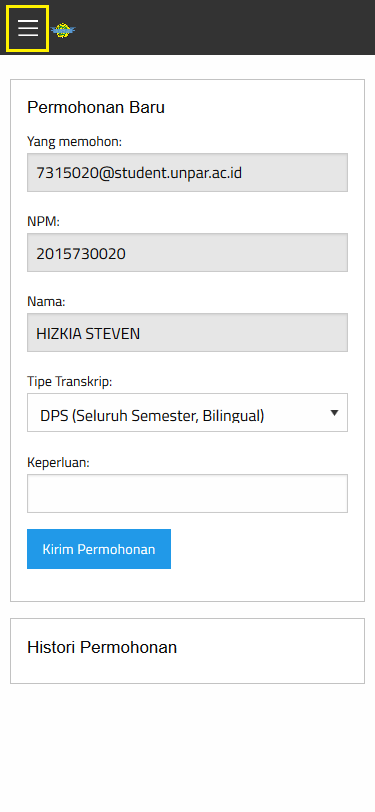
\includegraphics[scale=0.5]{kriteria-sukses-1-1-1-non-text-content}  
    \caption[Kriteria Sukses 1.1.1 - Tombol Tanpa Nama]{Kriteria Sukses 1.1.1 - Tombol Tanpa Nama}
    \label{fig:1.1.1_non_text_content}  
\end{figure} 
Contoh tautan untuk halaman yang bermasalah: 

\url{https://bluetape.azurewebsites.net/TranskripRequest}.

\subsubsection{\textit{Time-based Media}}
\label{subsubsec:kepatuhan_bluetape_time_based_media}

\paragraph{Kriteria Sukses 1.2.1 \textit{Audio-only and Video-only (Prerecorded)}}
\label{par:kepatuhan_bluetape_kriteria_sukses_1.2.1}
(Sukses)\\

Kriteria ini sukses dipatuhi karena pada halaman web BlueTape tidak terdapat konten media berbasis waktu.

\paragraph{Kriteria Sukses 1.2.2 \textit{Captions (Prerecorded)}}
\label{par:kepatuhan_bluetape_kriteria_sukses_1.2.2}
(Sukses)\\

Kriteria ini sukses dipatuhi karena pada halaman web BlueTape tidak terdapat konten media berbasis waktu.

\paragraph{Kriteria Sukses 1.2.3 \textit{Audio Description or Media Alternative (Prerecorded)}}
\label{par:kepatuhan_bluetape_kriteria_sukses_1.2.3}
(Sukses)\\

Kriteria ini sukses dipatuhi karena pada halaman web BlueTape tidak terdapat konten media berbasis waktu.

\paragraph{Kriteria Sukses 1.2.4 \textit{Captions (Live)}}
\label{par:kepatuhan_bluetape_kriteria_sukses_1.2.4}
(Sukses)\\

Kriteria ini sukses dipatuhi karena pada halaman web BlueTape tidak terdapat konten media berbasis waktu.

\paragraph{Kriteria Sukses 1.2.5 \textit{Audio Description (Prerecorded)}}
\label{par:kepatuhan_bluetape_kriteria_sukses_1.2.5}
(Sukses)\\

Kriteria ini sukses dipatuhi karena pada halaman web BlueTape tidak terdapat konten media berbasis waktu.

\paragraph{Kriteria Sukses 1.2.6 \textit{Sign Language (Prerecorded)}}
\label{par:kepatuhan_bluetape_kriteria_sukses_1.2.6}
(Sukses)\\

Kriteria ini sukses dipatuhi karena pada halaman web BlueTape tidak terdapat konten media berbasis waktu.

\paragraph{Kriteria Sukses 1.2.7 \textit{Extended Audio Description (Prerecorded)}}
\label{par:kepatuhan_bluetape_kriteria_sukses_1.2.7}
(Sukses)\\

Kriteria ini sukses dipatuhi karena pada halaman web BlueTape tidak terdapat konten media berbasis waktu.

\paragraph{Kriteria Sukses 1.2.8 \textit{Media Alternative (Prerecorded)}}
\label{par:kepatuhan_bluetape_kriteria_sukses_1.2.8}
(Sukses)\\

Kriteria ini sukses dipatuhi karena pada halaman web BlueTape tidak terdapat konten media berbasis waktu.

\paragraph{Kriteria Sukses 1.2.9 \textit{Audio-only (Live)}}
\label{par:kepatuhan_bluetape_kriteria_sukses_1.2.9}
(Sukses)\\

Kriteria ini sukses dipatuhi karena pada halaman web BlueTape tidak terdapat konten media berbasis waktu.

\subsubsection{\textit{Adaptable}}
\label{subsubsec:kepatuhan_bluetape_adaptable}

\paragraph{Kriteria Sukses 1.3.1 \textit{Info and Relationships}}
\label{par:kepatuhan_bluetape_kriteria_sukses_1.3.1}
(Tidak Sukses)\\

Kriteria ini tidak sukses dipatuhi karena:
\begin{itemize}
    \item Terdapat penggunaan \textit{tag heading} yang tidak tepat secara struktur pada halaman cetak transkrip, manajemen cetak transkrip, perubahan kuliah, manajemen perubahan kuliah, dan entri jadwal dosen. Contoh kesalahan dapat dilihat pada potongan kode \ref{lst:1.3.1_heading_tidak_tepat} yang menampilkan kesalahan penggunaan \textit{tag heading} pada halaman cetak transkrip.
    \begin{lstlisting}[frame=single, label={lst:1.3.1_heading_tidak_tepat}, language=HTML, caption=Kriteria Sukses 1.3.1 - Penggunaan \textit{Heading} Tidak Tepat]
        <div class="callout">
            <h5>Permohonan Baru</h5>
            <form method="POST" action="/TranskripRequest/add">
    \end{lstlisting}
    Contoh tautan untuk halaman yang bermasalah: 
    
    \url{https://bluetape.azurewebsites.net/TranskripRequest}.

    \item Pada halaman manajemen cetak transkrip, kolom masukan NPM tidak memiliki label atau \textit{aria-label} yang bersangkutan dengan kolom masukan tersebut. Kesalahan dapat dilihat pada potongan kode \ref{lst:1.3.1_label_masukan_manajemen_cetak_transkrip}.
    \begin{lstlisting}[frame=single, label={lst:1.3.1_label_masukan_manajemen_cetak_transkrip}, language=HTML, caption=Kriteria Sukses 1.3.1 - Tidak Terdapat Label pada Kolom Masukan di Halaman Manajemen Cetak Transkrip]
        <span class="input-group-label">Cari NPM:</span>
        <input name="npm" class="input-group-field" type="text"
        placeholder="2013730013" maxlength="10" minlength="10"/>
        <div class="input-group-button">
    \end{lstlisting}
    Tautan untuk halaman yang bermasalah: 
    
    \url{https://bluetape.azurewebsites.net/TranskripManage}.

    \item Pada halaman entri jadwal dosen, setiap kolom masukkan tidak memiliki label atau \textit{aria-label} yang bersangkutan dengan kolom-kolom masukan tersebut. Contoh kesalahan dapat dilihat pada potongan kode \ref{lst:1.3.1_label_masukan_entri_jadwal_dosen}.
    \begin{lstlisting}[frame=single, label={lst:1.3.1_label_masukan_entri_jadwal_dosen}, language=HTML, caption=Kriteria Sukses 1.3.1 - Tidak Terdapat Label pada Kolom Masukan di Halaman Entri Jadwal Dosen]
        <input type="hidden" name="csrf_token"
        value="3c159eae7bc953dd591b679c080ed066"/>
        Hari
        <select name="hari">
    \end{lstlisting}
    Tautan untuk halaman yang bermasalah: 
    
    \url{https://bluetape.azurewebsites.net/EntriJadwalDosen}.
\end{itemize} 

\paragraph{Kriteria Sukses 1.3.2 \textit{Meaningful Sequence}}
\label{par:kepatuhan_bluetape_kriteria_sukses_1.3.2}
(Sukses)\\

Kriteria ini sukses dipatuhi karena pada setiap halaman web BlueTape sudah memiiliki urutan membaca yang benar dan dapat ditentukan secara terprogram. 

\paragraph{Kriteria Sukses 1.3.3 \textit{Sensory Characteristics}}
\label{par:kepatuhan_bluetape_kriteria_sukses_1.3.3}
(Tidak Sukses)\\

Kriteria ini tidak sukses dipatuhi karena pada halaman cetak transkrip, manajemen cetak transkrip, perubahan kuliah, dan manajemen perubahan kuliah terdapat satu atau lebih komponen untuk mengoperasikan konten yang hanya mengandalkan satu komponen karakteristik indra yaitu bentuk. Komponen-komponen ini terletak pada kolom "Aksi" dan hanya ditampilkan dalam rupa ikon tanpa memiliki keterangan lebih detail. Contoh kesalahan dapat dilihat pada potongan kode \ref{lst:1.3.3_ikon_tanpa_keterangan}. Contoh tampilan pada halaman web dapat dilihat pada gambar \ref{fig:1.3.3_sensory_characteristics}.

\begin{lstlisting}[frame=single, label={lst:1.3.3_ikon_tanpa_keterangan}, language=HTML, caption=Kriteria Sukses 1.3.3 - Ikon Tanpa Keterangan]
    <td>
        <a data-open="detail12">
            <i class="fi-eye"></i>
        </a>
        <a target="_blank" 
        href="/PerubahanKuliahManage/printview/12">
            <i class="fi-print"></i>
        </a>
        <a data-open="konfirmasi12">
            <i class="fi-like"></i>
        </a>  
        <a data-open="tolak12">
            <i class="fi-dislike"></i>
        </a>
        <a data-open="hapus12">
            <i class="fi-trash"></i>
        </a>
    </td>
\end{lstlisting}

\begin{figure}[H]
	\centering  
	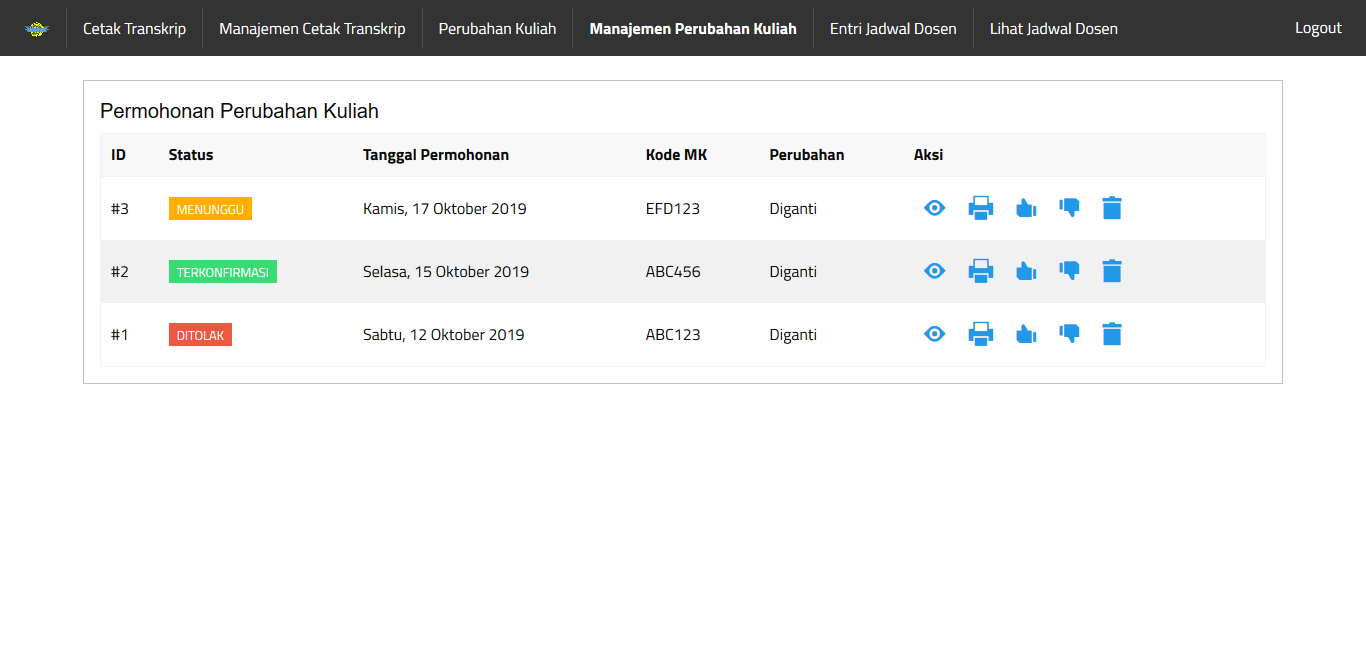
\includegraphics[scale=0.5]{kriteria-sukses-1-3-3-sensory-characteristics}  
    \caption[Kriteria Sukses 1.3.3 - Ikon pada Bagian Aksi]{Kriteria Sukses 1.3.3 - Ikon pada Bagian Aksi}
    \label{fig:1.3.3_sensory_characteristics}  
\end{figure} 
Contoh tautan untuk halaman yang bermasalah: 

\url{https://bluetape.azurewebsites.net/PerubahanKuliahManage}.

\paragraph{Kriteria Sukses 1.3.4 \textit{Orientation}}
\label{par:kepatuhan_bluetape_kriteria_sukses_1.3.4}
(Sukses)\\

Kriteria ini sukses dipatuhi karena konten pada halaman web BlueTape dapat disajikan dalam orientasi \textit{portrait} maupun \textit{landscape}.

\paragraph{Kriteria Sukses 1.3.5 \textit{Identify Input Purpose}}
\label{par:kepatuhan_bluetape_kriteria_sukses_1.3.5}
(Tidak Sukses)\\

Kriteria ini tidak sukses dipatuhi karena terdapat kolom-kolom masukan yang tidak memiliki label yang terasosiasi dengan kolom-kolom tersebut, meskipun setiap kolom masukan sudah memiliki atribut \textit{"autocomplete"} yang aktif. Bagian-bagian yang bermasalah, antara lain:
\begin{itemize}
    \item Pada halaman manajemen cetak transkrip, kolom masukan NPM tidak memiliki label atau \textit{aria-label} yang bersangkutan dengan kolom masukan tersebut. Kesalahan dapat dilihat pada potongan kode \ref{lst:1.3.5_label_masukan_manajemen_cetak_transkrip}.
    \begin{lstlisting}[frame=single, label={lst:1.3.5_label_masukan_manajemen_cetak_transkrip}, language=HTML, caption=Kriteria Sukses 1.3.5 - Tidak Terdapat Label pada Kolom Masukan di Halaman Manajemen Cetak Transkrip]
        <span class="input-group-label">Cari NPM:</span>
        <input name="npm" class="input-group-field" type="text"
        placeholder="2013730013" maxlength="10" minlength="10"/>
        <div class="input-group-button">
    \end{lstlisting}
    Tautan untuk halaman yang bermasalah: 
    
    \url{https://bluetape.azurewebsites.net/TranskripManage}.

    \item Pada halaman entri jadwal dosen, setiap kolom masukkan tidak memiliki label atau \textit{aria-label} yang bersangkutan dengan kolom-kolom masukan tersebut. Contoh kesalahan dapat dilihat pada potongan kode \ref{lst:1.3.5_label_masukan_entri_jadwal_dosen}.
    \begin{lstlisting}[frame=single, label={lst:1.3.5_label_masukan_entri_jadwal_dosen}, language=HTML, caption=Kriteria Sukses 1.3.5 - Tidak Terdapat Label pada Kolom Masukan di Halaman Entri Jadwal Dosen]
        <input type="hidden" 
        name="csrf_token"
        value="3c159eae7bc953dd591b679c080ed066" />
        Hari
        <select name="hari">
    \end{lstlisting}
    Tautan untuk halaman yang bermasalah: 
    
    \url{https://bluetape.azurewebsites.net/EntriJadwalDosen}.
\end{itemize}

\paragraph{Kriteria Sukses 1.3.6 \textit{Identify Purpose}}
\label{par:kepatuhan_bluetape_kriteria_sukses_1.3.6}
(Tidak Sukses)\\

Kriteria ini tidak sukses dipatuhi karena terdapat elemen \textit{HTML}5 yang seharusnya dapat digunakan namun tidak digunakan, contohnya pada bagian navigasi. Kesalahan dapat dilihat pada potongan kode \ref{lst:1.3.6_navigasi}.

\begin{lstlisting}[frame=single, label={lst:1.3.6_navigasi}, language=HTML, caption=Kriteria Sukses 1.3.6 - Navigasi]
    </div>
    <div class="top-bar" id="navigation-menu">
        <div class="top-bar-left">
\end{lstlisting}

\subsubsection{\textit{Distinguishable}}
\label{subsubsec:kepatuhan_bluetape_distinguishable}

\paragraph{Kriteria Sukses 1.4.1 \textit{Use of Color}}
\label{par:kepatuhan_bluetape_kriteria_sukses_1.4.1}
(Sukses)\\

Kriteria ini sukses dipatuhi karena pada halaman web BlueTape, warna tidak digunakan sebagai satu-satunya cara untuk menyampaikan informasi secara visual, menandai suatu tindakan, meminta respons, atau membedakan elemen visual.

\paragraph{Kriteria Sukses 1.4.2 \textit{Audio Control}}
\label{par:kepatuhan_bluetape_kriteria_sukses_1.4.2}
(Sukses)\\

Kriteria ini sukses dipatuhi karena pada halaman web BlueTape tidak terdapat konten media berbasis waktu.

\paragraph{Kriteria Sukses 1.4.3 \textit{Contrast (Minimum)}}
\label{par:kepatuhan_bluetape_kriteria_sukses_1.4.3}
(Tidak Sukses)\\

Kriteria ini tidak sukses dipatuhi karena pada halaman web BlueTape terdapat beberapa teks dengan rasio kontras kurang dari 4,5:1 untuk teks yang berukuran kurang dari 24 piksel dan tidak \textit{bold}, antara lain:

\begin{itemize}
    \item Halaman \textit{login}: Teks "\textit{Login} dengan Google" memiliki rasio kontras 3.09:1 terhadap warna latar belakangnya. Teks "Petunjuk Penggunaan" memiliki rasio kontras 3.06:1 terhadap warna latar belakangnya. Tampilan pada halaman web dapat dilihat pada gambar \ref{fig:1.4.3_contrast_minimum_1}.
    \begin{figure}[H]
        \centering  
        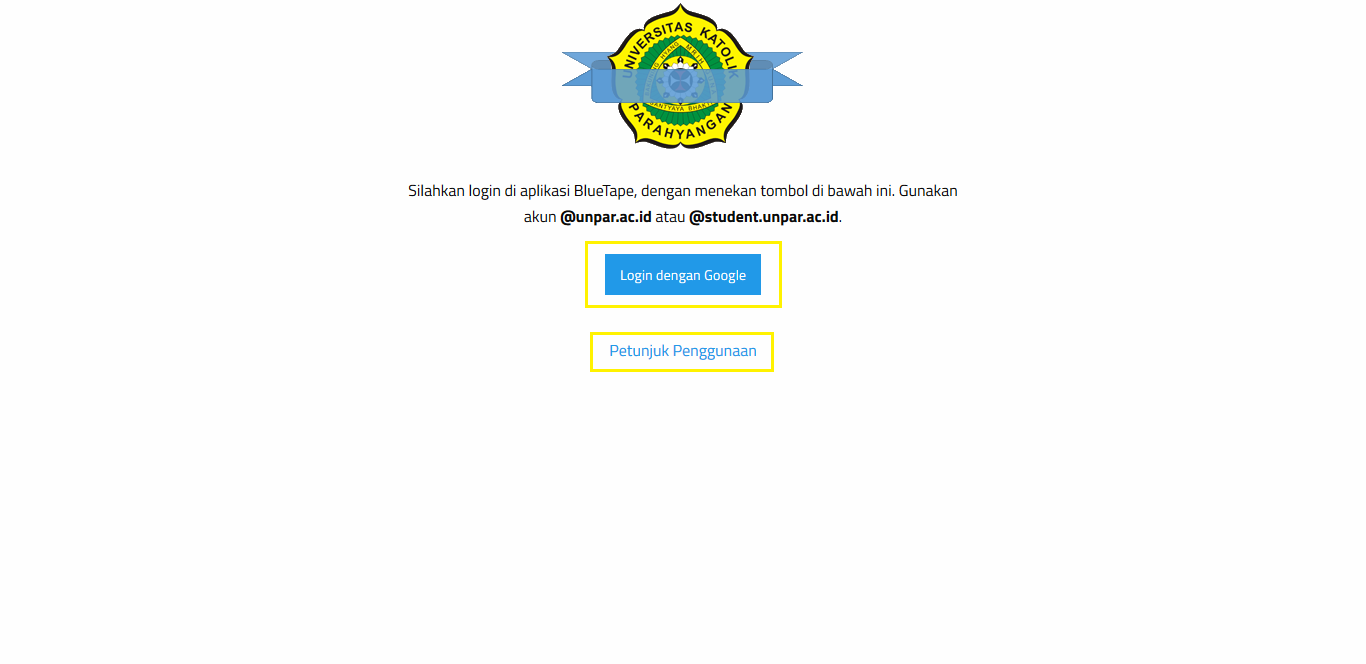
\includegraphics[scale=0.5]{kriteria-sukses-1-4-3-contrast-minimum-1}  
        \caption[Kriteria Sukses 1.4.3 - Kontras Elemen pada Halaman \textit{login}]{Kriteria Sukses 1.4.3 - Kontras Elemen pada Halaman \textit{login}}
        \label{fig:1.4.3_contrast_minimum_1}  
    \end{figure} 
    Tautan untuk halaman yang bermasalah: 
    
    \url{https://bluetape.azurewebsites.net}.

    \item Halaman cetak transkrip: Teks "Kirim Permohonan" memiliki rasio kontras 3.09:1 terhadap warna latar belakangnya. Teks "Tercetak" di kolom status pada tabel memiliki rasio kontras 1,79:1 terhadap warna latar belakangnya. Teks "Ditolak" di kolom status pada tabel "Histori Permohonan" memiliki rasio kontras 3,44:1 terhadap warna latar belakangnya. Teks "Tunggu" di kolom status pada tabel "Histori Permohonan" memiliki rasio kontras 4,44:1 terhadap warna latar belakangnya. Tampilan pada halaman web dapat dilihat pada gambar \ref{fig:1.4.3_contrast_minimum_2}.
    \begin{figure}[H]
        \centering  
        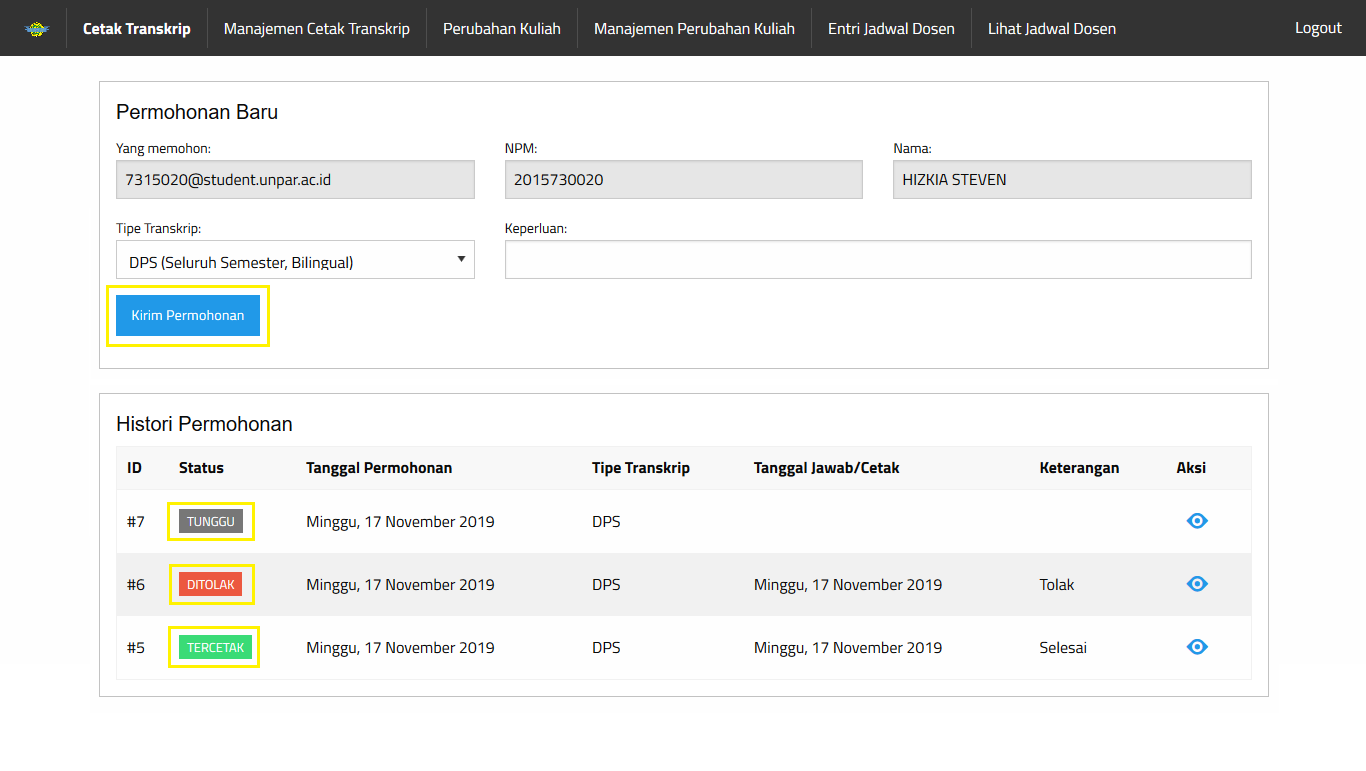
\includegraphics[scale=0.5]{kriteria-sukses-1-4-3-contrast-minimum-2}  
        \caption[Kriteria Sukses 1.4.3 - Kontras Elemen pada Halaman Cetak Transkrip]{Kriteria Sukses 1.4.3 - Kontras Elemen pada Halaman Cetak Transkrip}
        \label{fig:1.4.3_contrast_minimum_2}  
    \end{figure} 
    Tautan untuk halaman yang bermasalah: 
    
    \url{https://bluetape.azurewebsites.net/TranskripRequest}.

    \item Halaman manajemen cetak transkrip: Teks "Cari" memiliki rasio kontras 3.09:1 terhadap warna latar belakangnya. Teks "Tercetak" di kolom status pada tabel memiliki rasio kontras 1,79:1 terhadap warna latar belakangnya. Teks "Menunggu" di kolom status pada tabel memiliki rasio kontras 1,84:1 terhadap warna latar belakangnya. Teks "Ditolak" di kolom status pada tabel memiliki rasio kontras 3,44:1 terhadap warna latar belakangnya. Teks "Hapus" pada bagian hapus permohonan memiliki rasio kontras 3,47:1 terhadap warna latar belakangnya. Tampilan pada halaman web dapat dilihat pada gambar \ref{fig:1.4.3_contrast_minimum_3}.
    \begin{figure}[H]
        \centering  
        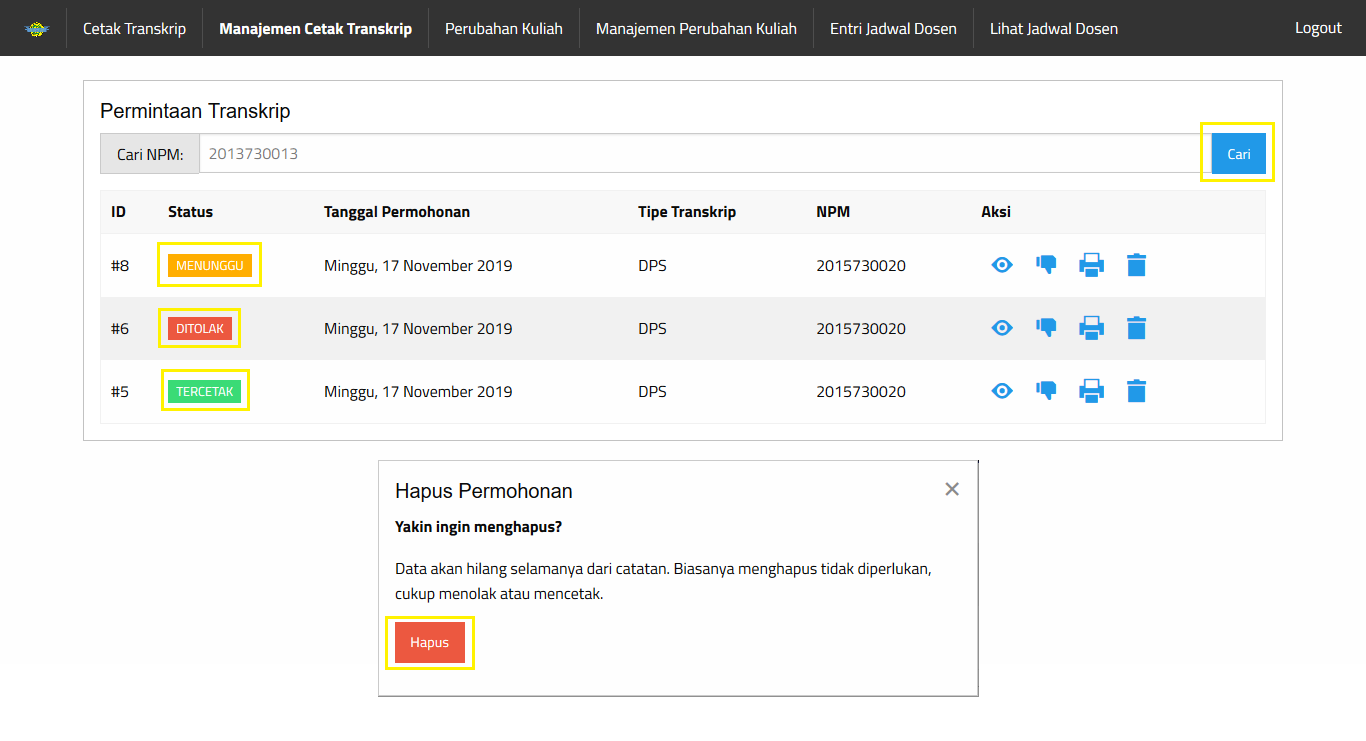
\includegraphics[scale=0.5]{kriteria-sukses-1-4-3-contrast-minimum-3}  
        \caption[Kriteria Sukses 1.4.3 - Kontras Elemen pada Halaman Manajemen Cetak Transkrip]{Kriteria Sukses 1.4.3 - Kontras Elemen pada Halaman Manajemen Cetak Transkrip}
        \label{fig:1.4.3_contrast_minimum_3}  
    \end{figure} 
    Tautan untuk halaman yang bermasalah: 
    
    \url{https://bluetape.azurewebsites.net/TranskripManage}.

    \item Halaman perubahan kuliah: Teks "Kirim Permohonan" memiliki rasio kontras 3.09:1 terhadap warna latar belakangnya. Teks "Tambah Pertemuan Ekstra" memiliki rasio kontras 4,47:1 terhadap warna latar belakangnya. Teks "Hapus" memiliki rasio kontras 4,47:1 terhadap warna latar belakangnya. Teks "Tunggu" di kolom status pada tabel "Histori Permohonan" memiliki rasio kontras 4,44:1 terhadap warna latar belakangnya. Teks "Ditolak" di kolom status pada tabel "Histori Permohonan" memiliki rasio kontras 3,44:1 terhadap warna latar belakangnya. Teks "Terkonfirmasi" di kolom status pada tabel "Histori Permohonan" memiliki rasio kontras 1,79:1 terhadap warna latar belakangnya. Tampilan pada halaman web dapat dilihat pada gambar \ref{fig:1.4.3_contrast_minimum_4}.
    \begin{figure}[H]
        \centering  
        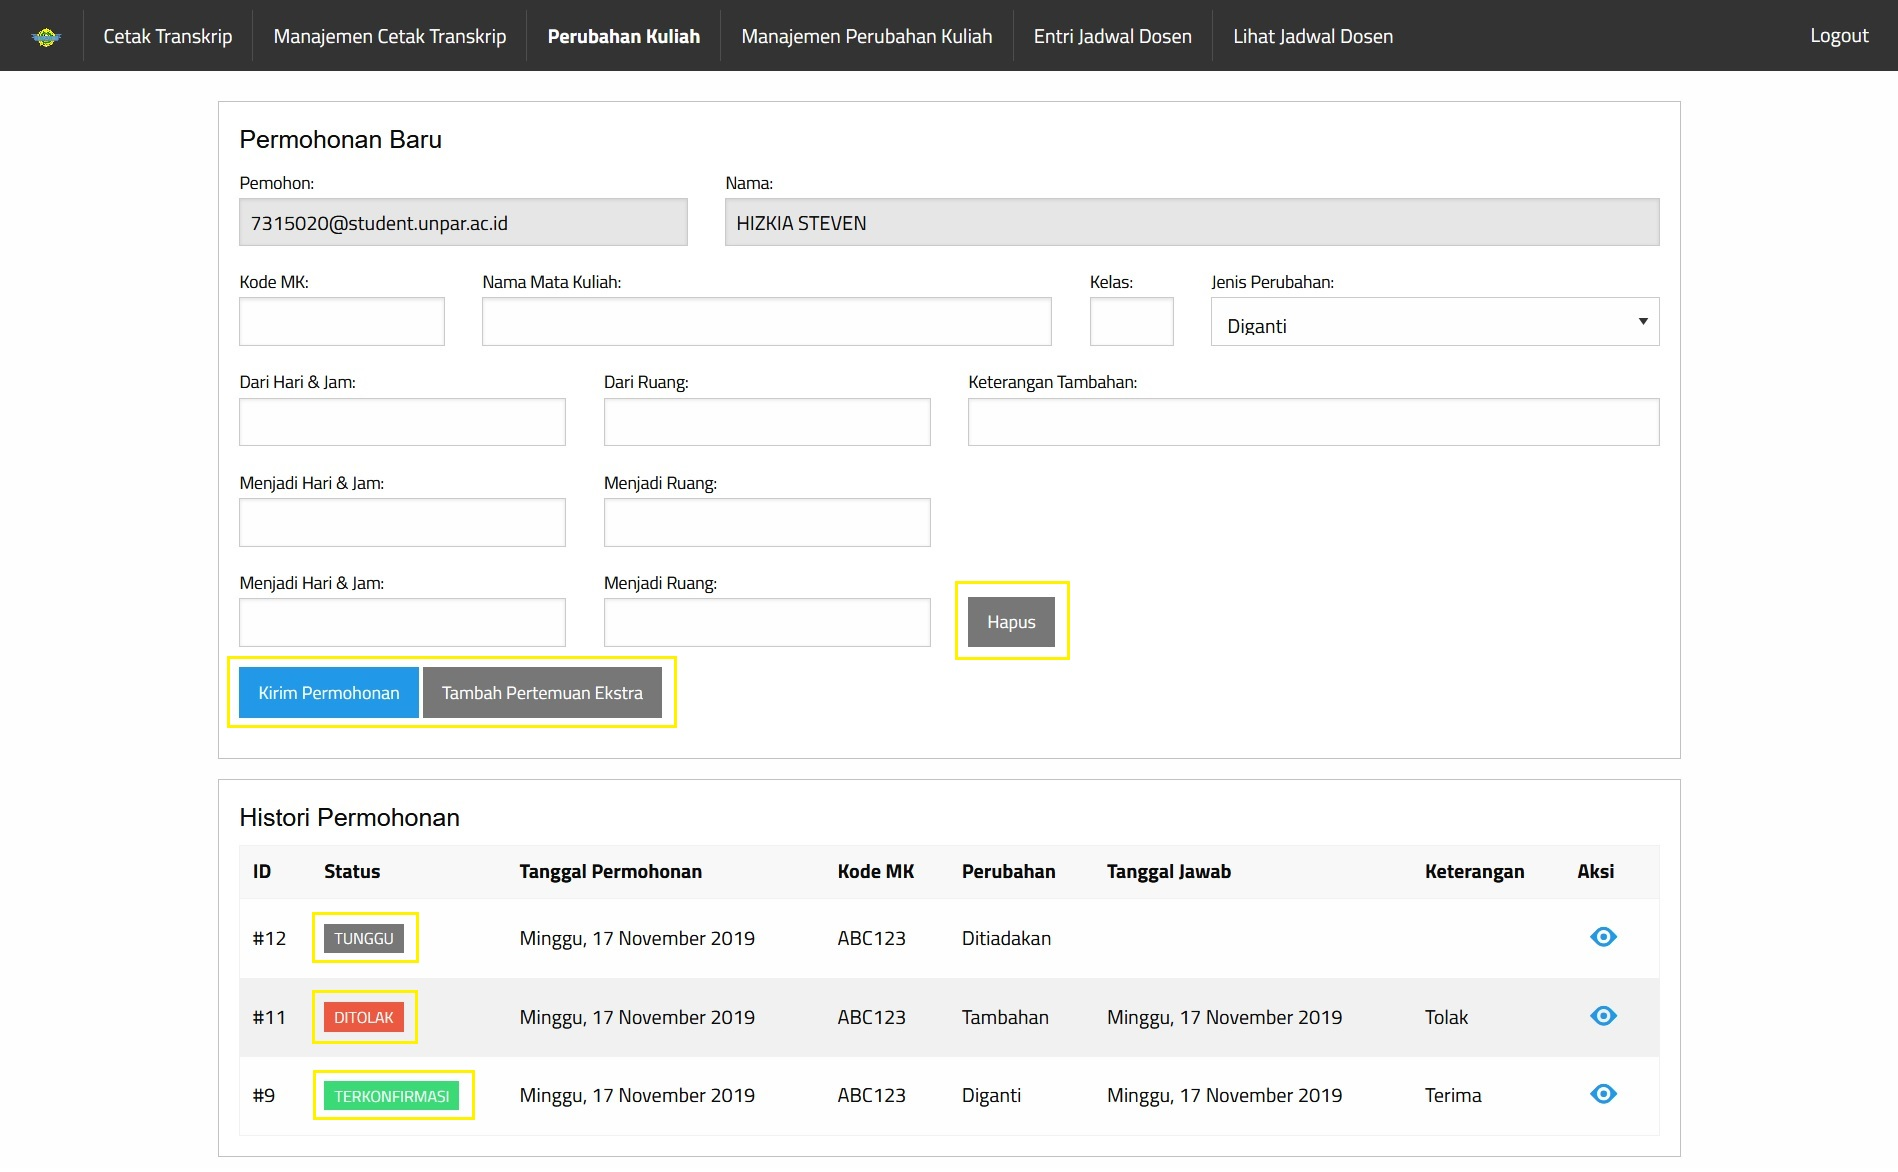
\includegraphics[scale=0.5]{kriteria-sukses-1-4-3-contrast-minimum-4}  
        \caption[Kriteria Sukses 1.4.3 - Kontras Elemen pada Halaman Perubahan Kuliah]{Kriteria Sukses 1.4.3 - Kontras Elemen pada Halaman Perubahan Kuliah}
        \label{fig:1.4.3_contrast_minimum_4}  
    \end{figure} 
    Tautan untuk halaman yang bermasalah: 

    \url{https://bluetape.azurewebsites.net/PerubahanKuliahRequest}.
    
    \item Halaman manajemen perubahan kuliah: Teks "Terkonfirmasi" di kolom status pada tabel memiliki rasio kontras 1,79:1 terhadap warna latar belakangnya. Teks "Menunggu" di kolom status pada tabel memiliki rasio kontras 1,84:1 terhadap warna latar belakangnya. Teks "Ditolak" di kolom status pada tabel memiliki rasio kontras 3,44:1 terhadap warna latar belakangnya. Teks "Hapus" pada bagian hapus permohonan memiliki rasio kontras 3,47:1 terhadap warna latar belakangnya. Tampilan pada halaman web dapat dilihat pada gambar \ref{fig:1.4.3_contrast_minimum_5}.
    \begin{figure}[H]
        \centering  
        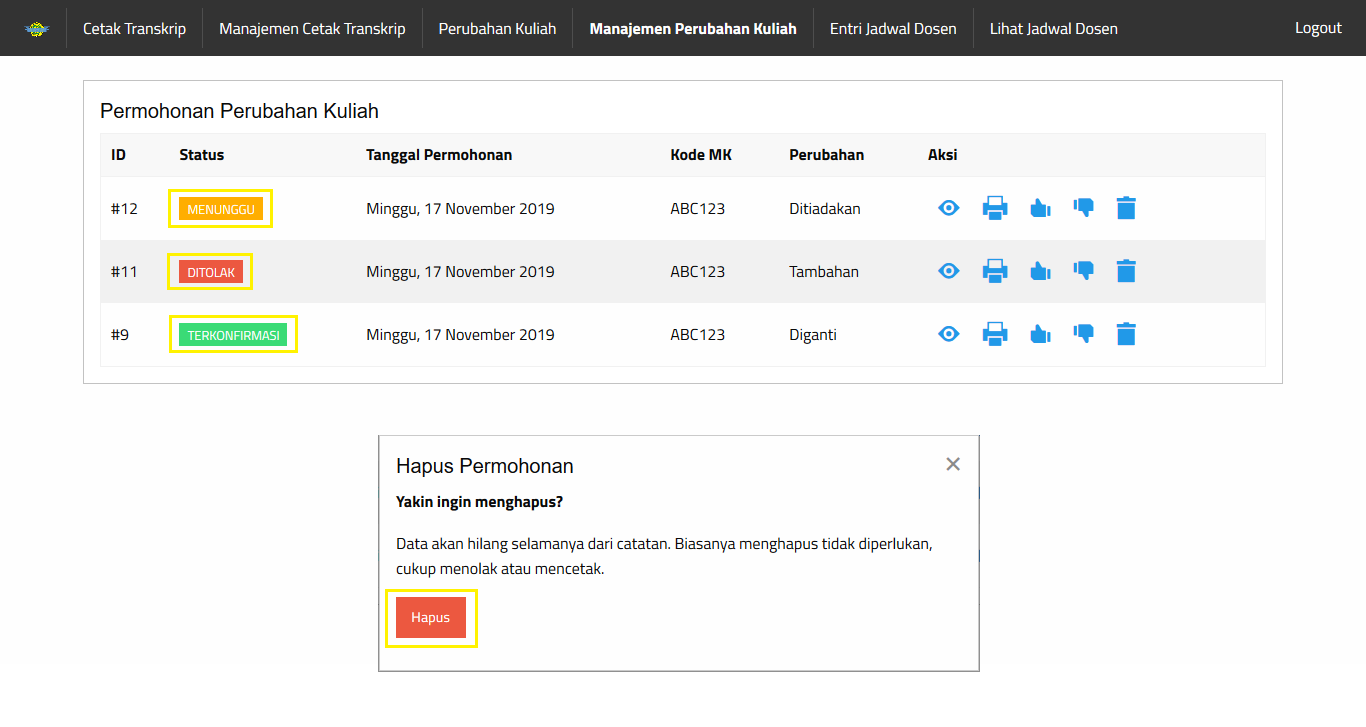
\includegraphics[scale=0.5]{kriteria-sukses-1-4-3-contrast-minimum-5}  
        \caption[Kriteria Sukses 1.4.3 - Kontras Elemen pada Halaman Manajemen Perubahan Kuliah]{Kriteria Sukses 1.4.3 - Kontras Elemen pada Halaman Manajemen Perubahan Kuliah}
        \label{fig:1.4.3_contrast_minimum_5}  
    \end{figure} 
    Tautan untuk halaman yang bermasalah: 
    
    \url{https://bluetape.azurewebsites.net/PerubahanKuliahManage}.

    \item Halaman entri jadwal dosen: Teks "Tambah" memiliki rasio kontras 3.09:1 terhadap warna latar belakangnya. Teks "Delete All" memiliki rasio kontras 3.47:1 terhadap warna latar belakangnya. Teks "Ekspor ke XLS" memiliki rasio kontras 3.09:1 terhadap warna latar belakangnya. Teks "Save" pada bagian "Edit Jadwal" memiliki rasio kontras 3.09:1 terhadap warna latar belakangnya. Teks "Delete" memiliki rasio kontras 3.47:1 terhadap warna latar belakangnya. Tampilan pada halaman web dapat dilihat pada gambar \ref{fig:1.4.3_contrast_minimum_6}.
    \begin{figure}[H]
        \centering  
        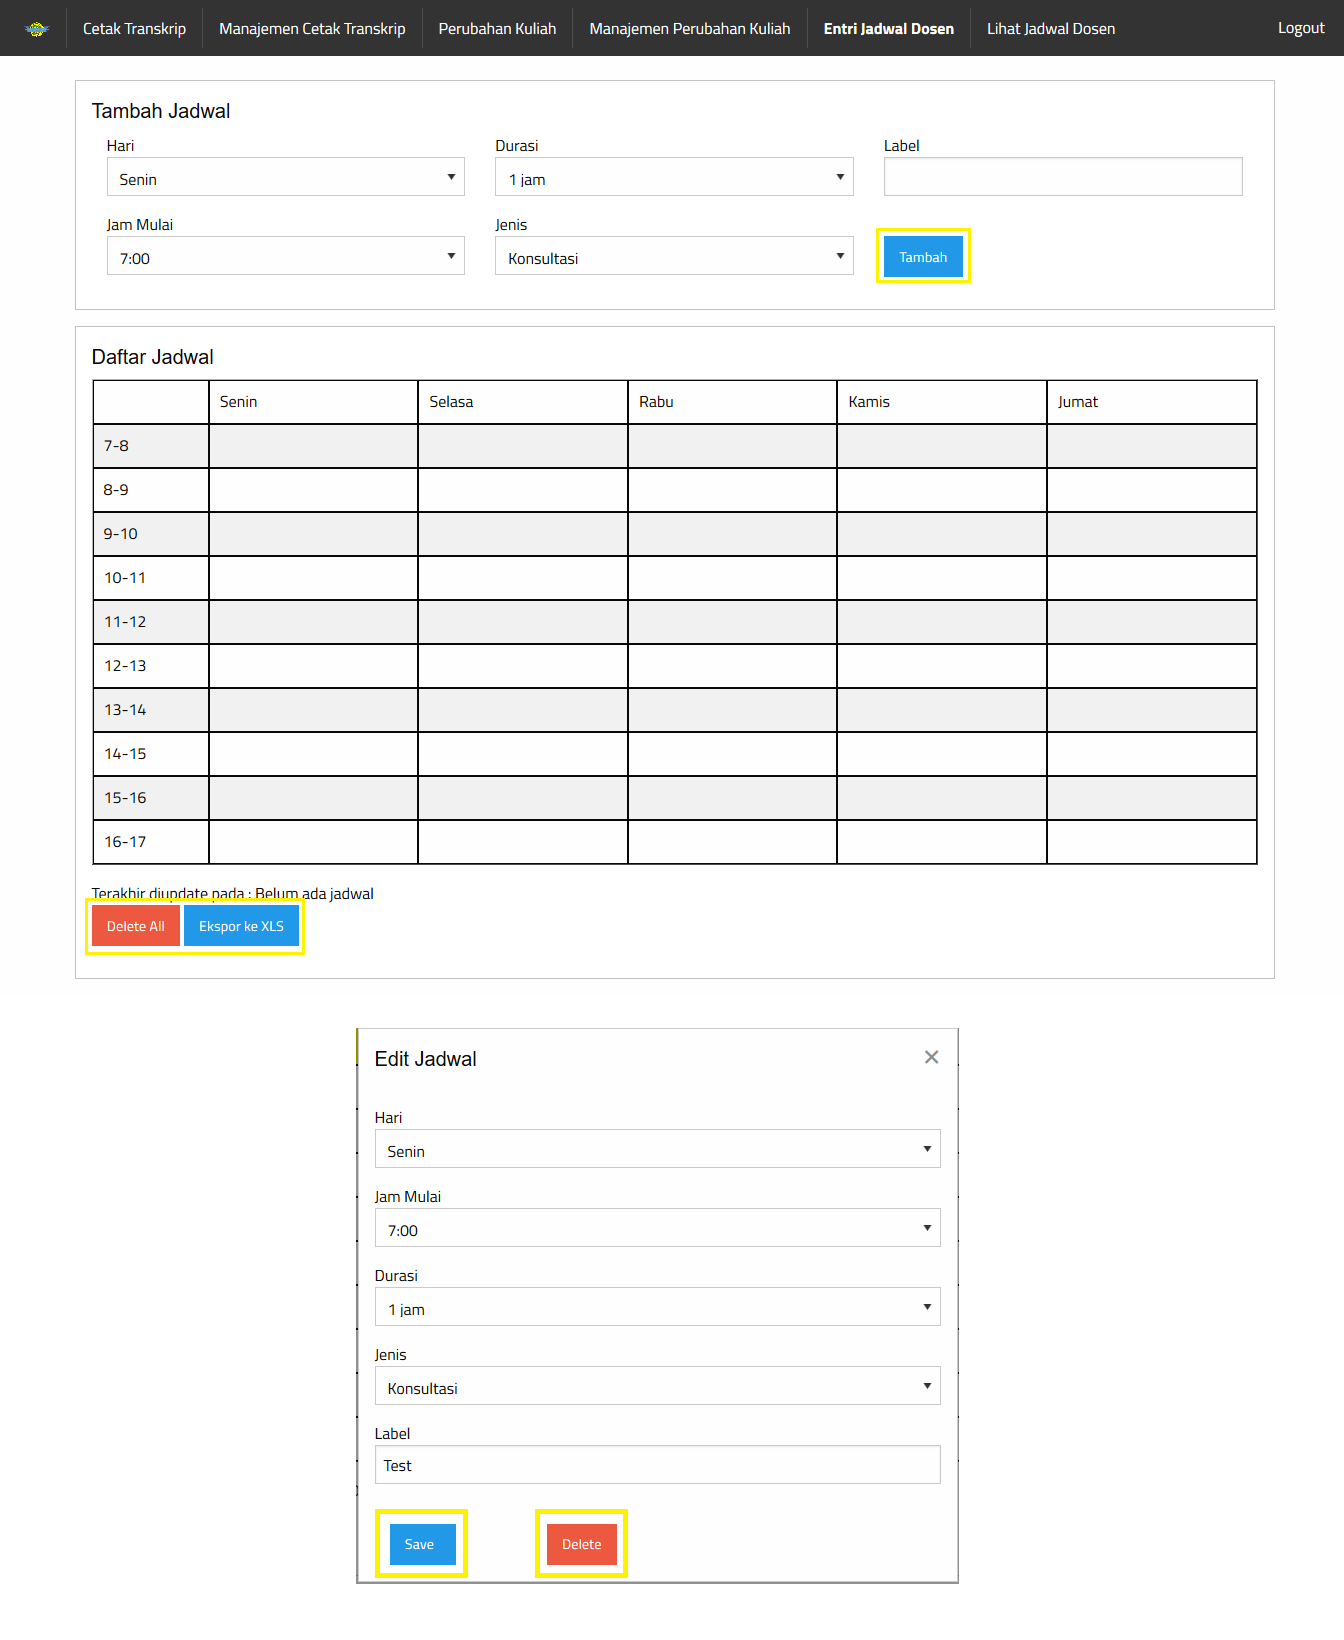
\includegraphics[scale=0.5]{kriteria-sukses-1-4-3-contrast-minimum-6}  
        \caption[Kriteria Sukses 1.4.3 - Kontras Elemen pada Halaman Entri Jadwal Dosen]{Kriteria Sukses 1.4.3 - Kontras Elemen pada Halaman Entri Jadwal Dosen}
        \label{fig:1.4.3_contrast_minimum_6}  
    \end{figure} 
    Tautan untuk halaman yang bermasalah: 
    
    \url{https://bluetape.azurewebsites.net/EntriJadwalDosen}.
    
    \item Halaman lihat jadwal dosen: Teks nama dosen di atas tabel yang sedang dipilih pengguna memiliki rasio kontras 2,47:1 terhadap warna latar belakangnya. Teks nama dosen di atas tabel yang sedang tidak dipilih pengguna memiliki rasio kontras 3,06:1 terhadap warna latar belakangnya. Teks "Ekspor ke XLS" memiliki rasio kontras 3.09:1 terhadap warna latar belakangnya. Tampilan pada halaman web dapat dilihat pada gambar \ref{fig:1.4.3_contrast_minimum_7}.
    \begin{figure}[H]
        \centering  
        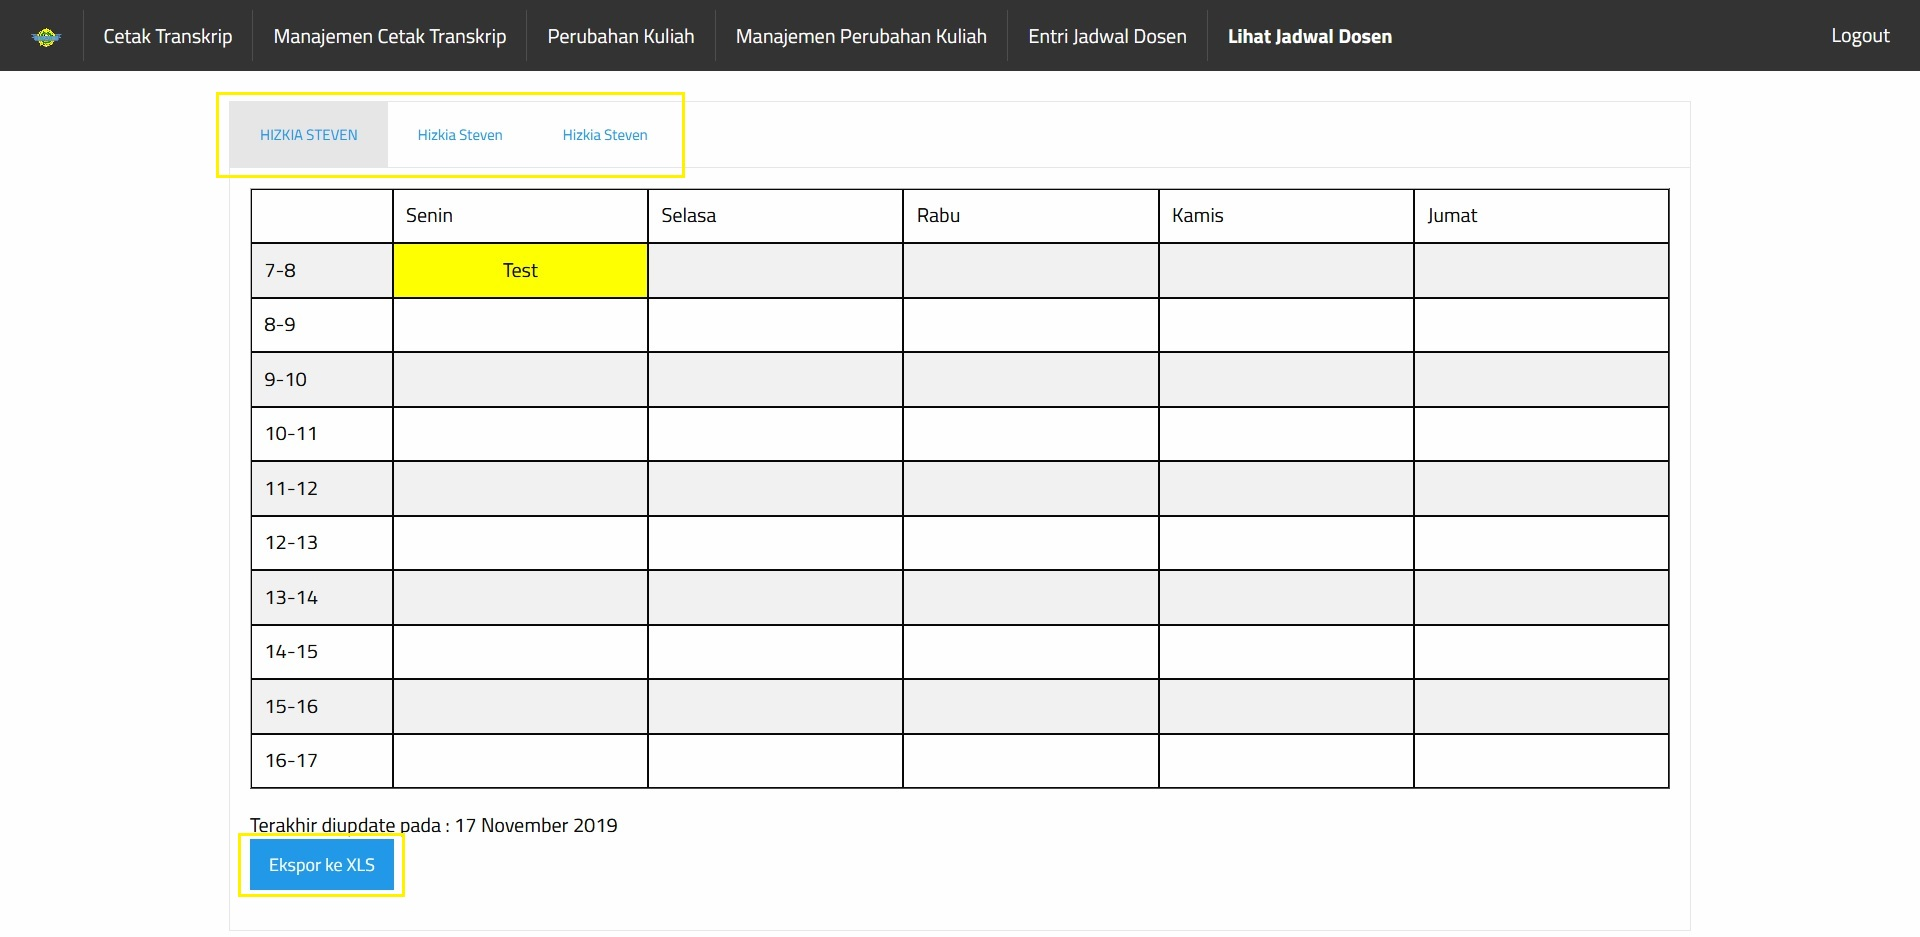
\includegraphics[scale=0.5]{kriteria-sukses-1-4-3-contrast-minimum-7}  
        \caption[Kriteria Sukses 1.4.3 - Kontras Elemen pada Halaman Lihat Jadwal Dosen]{Kriteria Sukses 1.4.3 - Kontras Elemen pada Halaman Lihat Jadwal Dosen}
        \label{fig:1.4.3_contrast_minimum_7}  
    \end{figure} 
    Tautan untuk halaman yang bermasalah: 
    
    \url{https://bluetape.azurewebsites.net/LihatJadwalDosen}.
\end{itemize}

\paragraph{Kriteria Sukses 1.4.4 \textit{Resize text}}
\label{par:kepatuhan_bluetape_kriteria_sukses_1.4.4}
(Sukses)\\

Kriteria ini sukses dipatuhi karena setiap halaman web BlueTape dapat tetap terbaca dan tidak kehilangan fungsionalitasnya ketika halaman diperbesar hingga 200 persen. 

\paragraph{Kriteria Sukses 1.4.5 \textit{Images of Text}}
\label{par:kepatuhan_bluetape_kriteria_sukses_1.4.5}
(Sukses)\\

Kriteria ini sukses dipatuhi karena pada halaman web BlueTape tidak terdapat gambar teks selain logo.

\paragraph{Kriteria Sukses 1.4.6 \textit{Contrast (Enhanced)}}
\label{par:kepatuhan_bluetape_kriteria_sukses_1.4.6}
(Tidak Sukses)\\

Kriteria ini tidak sukses dipatuhi karena pada halaman web BlueTape terdapat beberapa teks dengan rasio kontras kurang dari 7:1 untuk teks yang berukuran kurang dari 24 piksel dan tidak \textit{bold}, antara lain:

\begin{itemize}
    \item Halaman \textit{login}: Teks "\textit{Login} dengan Google" memiliki rasio kontras 3.09:1 terhadap warna latar belakangnya. Teks "Petunjuk Penggunaan" memiliki rasio kontras 3.06:1 terhadap warna latar belakangnya. Tampilan pada halaman web dapat dilihat pada gambar \ref{fig:1.4.6_contrast_enchanced_1}.
    \begin{figure}[H]
        \centering  
        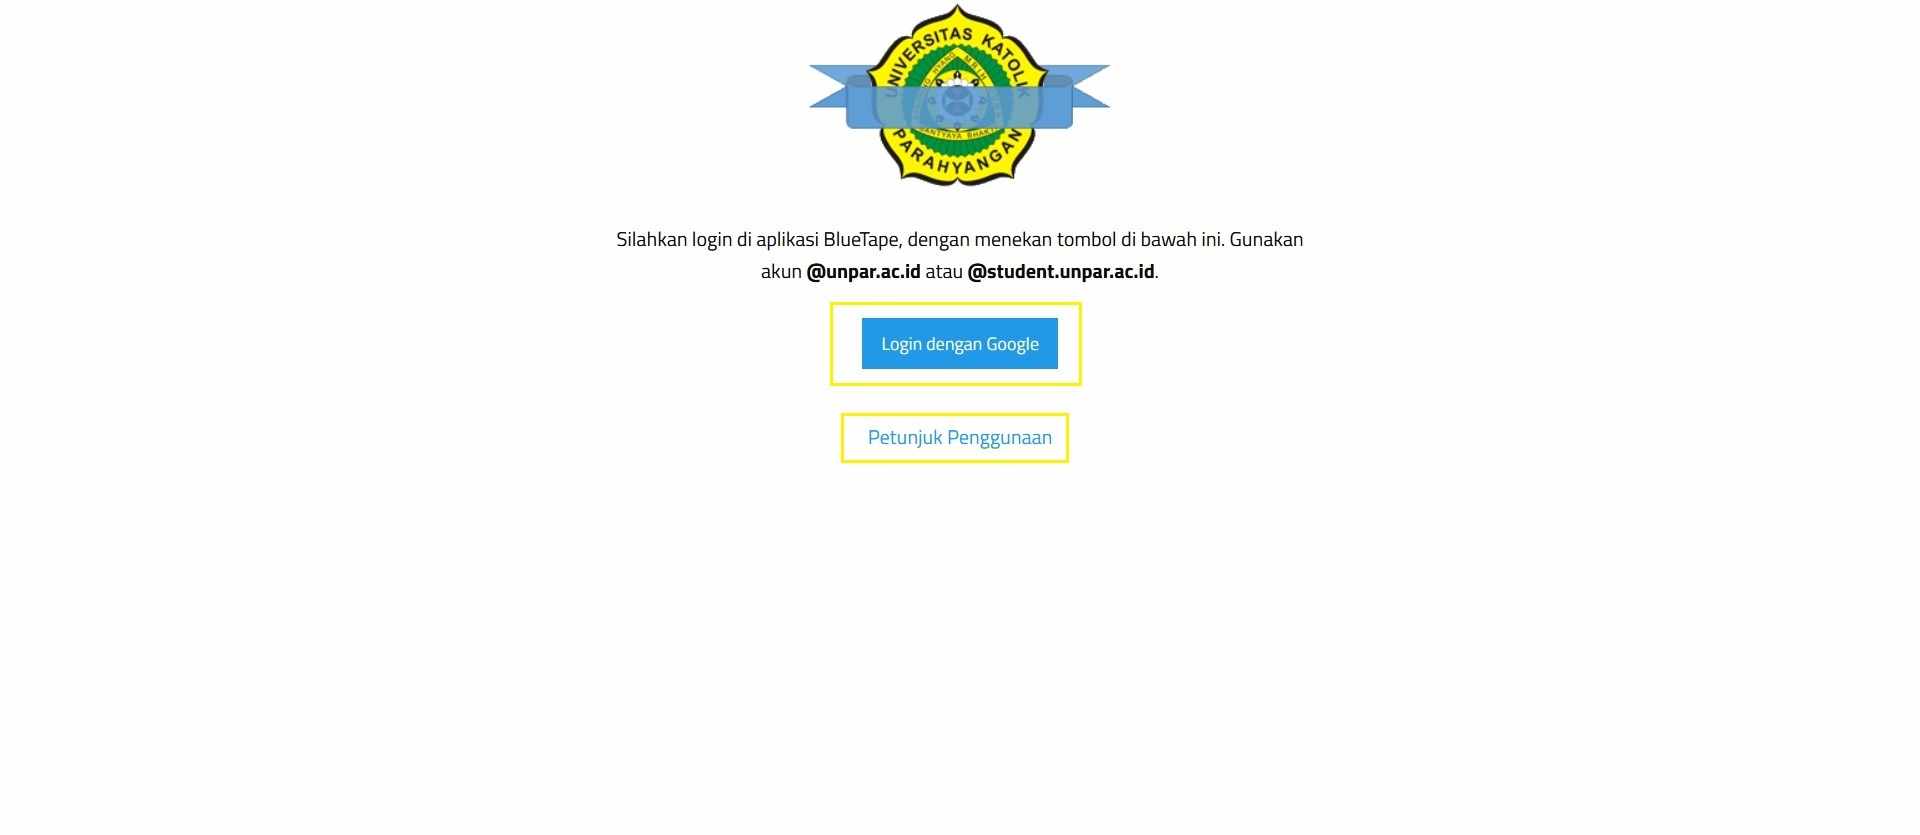
\includegraphics[scale=0.5]{kriteria-sukses-1-4-6-contrast-enchanced-1}  
        \caption[Kriteria Sukses 1.4.6 - Kontras Elemen pada Halaman \textit{login}]{Kriteria Sukses 1.4.6 - Kontras Elemen pada Halaman \textit{login}}
        \label{fig:1.4.6_contrast_enchanced_1}  
    \end{figure} 
    Tautan untuk halaman yang bermasalah: 
    
    \url{https://bluetape.azurewebsites.net}.

    \item Halaman cetak transkrip: Teks "Kirim Permohonan" memiliki rasio kontras 3.09:1 terhadap warna latar belakangnya. Teks "Tercetak" di kolom status pada tabel memiliki rasio kontras 1,79:1 terhadap warna latar belakangnya. Teks "Ditolak" di kolom status pada tabel "Histori Permohonan" memiliki rasio kontras 3,44:1 terhadap warna latar belakangnya. Teks "Tunggu" di kolom status pada tabel "Histori Permohonan" memiliki rasio kontras 4,44:1 terhadap warna latar belakangnya. Tampilan pada halaman web dapat dilihat pada gambar \ref{fig:1.4.6_contrast_enchanced_2}.
    \begin{figure}[H]
        \centering  
        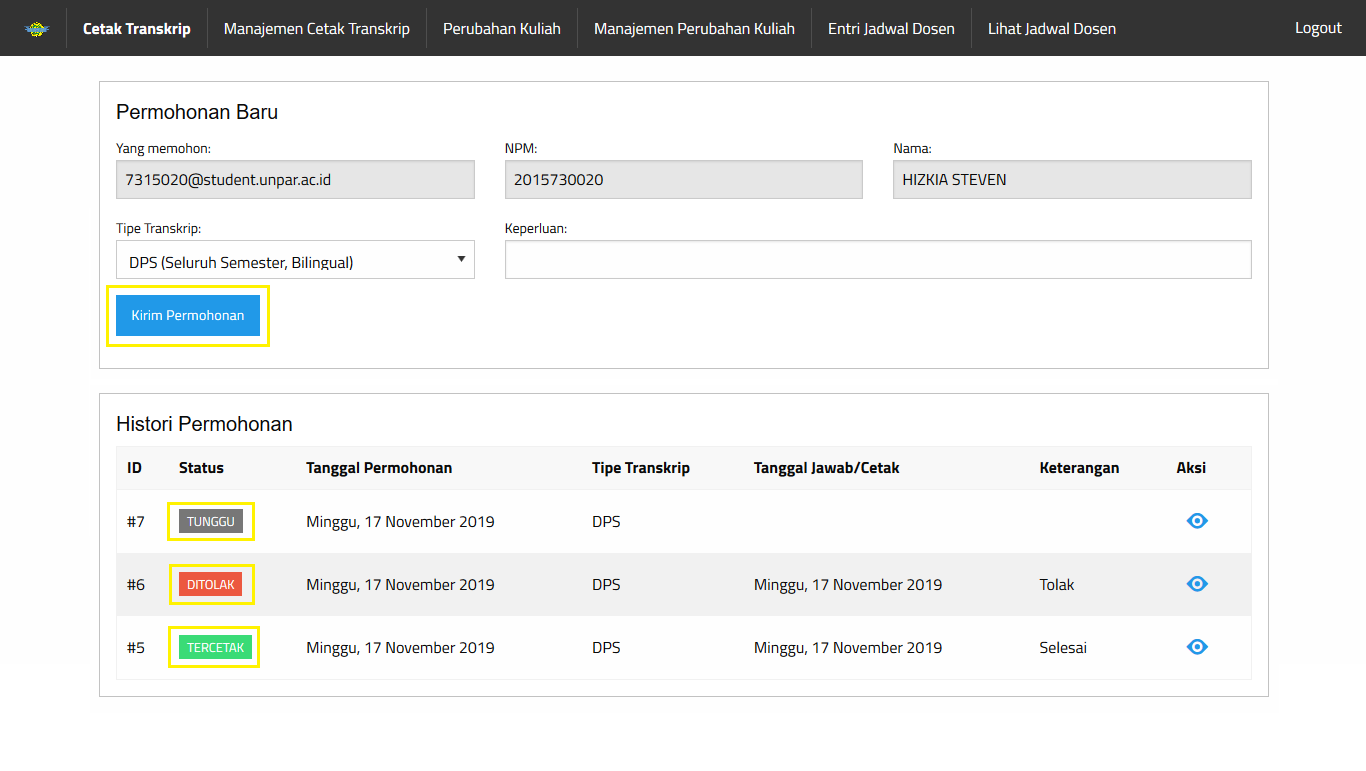
\includegraphics[scale=0.5]{kriteria-sukses-1-4-6-contrast-enchanced-2}  
        \caption[Kriteria Sukses 1.4.6 - Kontras Elemen pada Halaman Cetak Transkrip]{Kriteria Sukses 1.4.6 - Kontras Elemen pada Halaman Cetak Transkrip}
        \label{fig:1.4.6_contrast_enchanced_2}  
    \end{figure} 
    Tautan untuk halaman yang bermasalah: 
    
    \url{https://bluetape.azurewebsites.net/TranskripRequest}.

    \item Halaman manajemen cetak transkrip: Teks "Cari" memiliki rasio kontras 3.09:1 terhadap warna latar belakangnya. Teks "Tercetak" di kolom status pada tabel memiliki rasio kontras 1,79:1 terhadap warna latar belakangnya. Teks "Menunggu" di kolom status pada tabel memiliki rasio kontras 1,84:1 terhadap warna latar belakangnya. Teks "Ditolak" di kolom status pada tabel memiliki rasio kontras 3,44:1 terhadap warna latar belakangnya. Teks "Hapus" pada bagian hapus permohonan memiliki rasio kontras 3,47:1 terhadap warna latar belakangnya. Tampilan pada halaman web dapat dilihat pada gambar \ref{fig:1.4.6_contrast_enchanced_3}.
    \begin{figure}[H]
        \centering  
        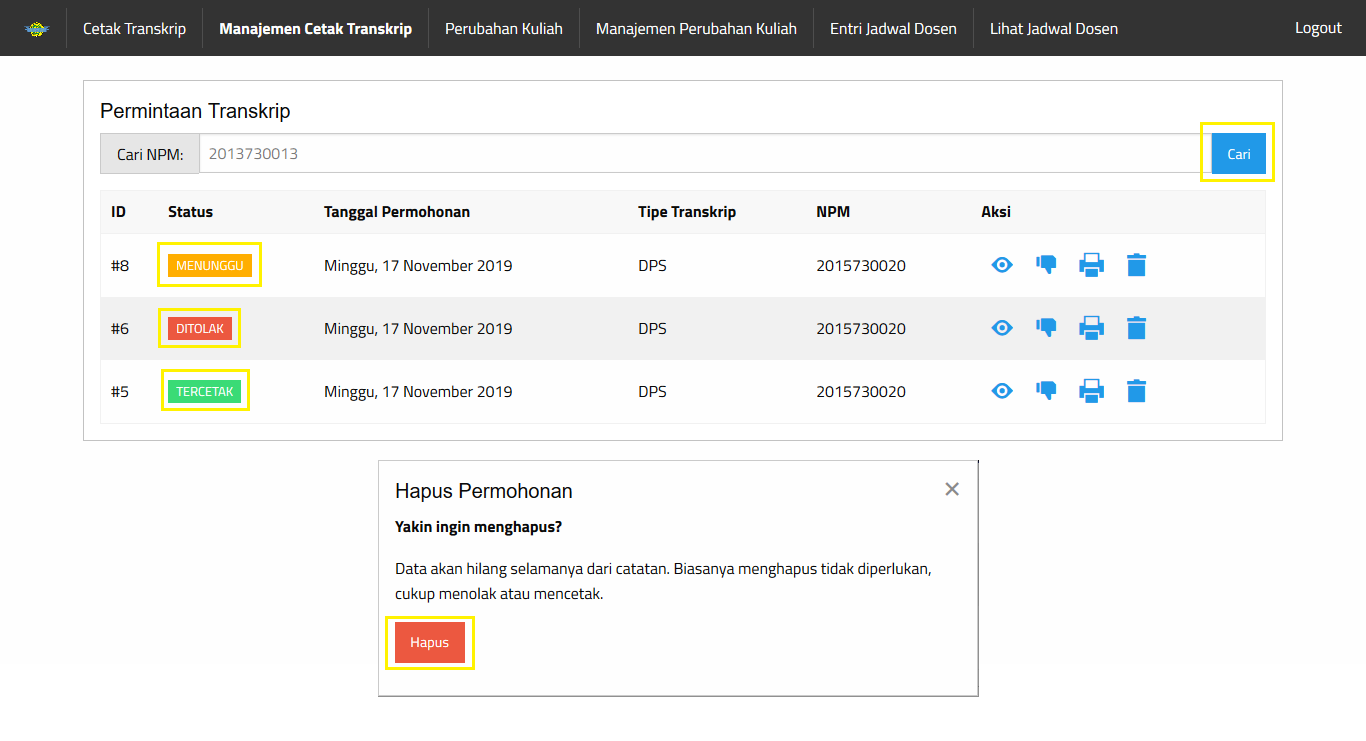
\includegraphics[scale=0.5]{kriteria-sukses-1-4-6-contrast-enchanced-3}  
        \caption[Kriteria Sukses 1.4.6 - Kontras Elemen pada Halaman Manajemen Cetak Transkrip]{Kriteria Sukses 1.4.6 - Kontras Elemen pada Halaman Manajemen Cetak Transkrip}
        \label{fig:1.4.6_contrast_enchanced_3}  
    \end{figure} 
    Tautan untuk halaman yang bermasalah: 
    
    \url{https://bluetape.azurewebsites.net/TranskripManage}.

    \item Halaman perubahan kuliah: Teks "Kirim Permohonan" memiliki rasio kontras 3.09:1 terhadap warna latar belakangnya. Teks "Tambah Pertemuan Ekstra" memiliki rasio kontras 4,47:1 terhadap warna latar belakangnya. Teks "Hapus" memiliki rasio kontras 4,47:1 terhadap warna latar belakangnya. Teks "Tunggu" di kolom status pada tabel "Histori Permohonan" memiliki rasio kontras 4,44:1 terhadap warna latar belakangnya. Teks "Ditolak" di kolom status pada tabel "Histori Permohonan" memiliki rasio kontras 3,44:1 terhadap warna latar belakangnya. Teks "Terkonfirmasi" di kolom status pada tabel "Histori Permohonan" memiliki rasio kontras 1,79:1 terhadap warna latar belakangnya. Tampilan pada halaman web dapat dilihat pada gambar \ref{fig:1.4.6_contrast_enchanced_4}.
    \begin{figure}[H]
        \centering  
        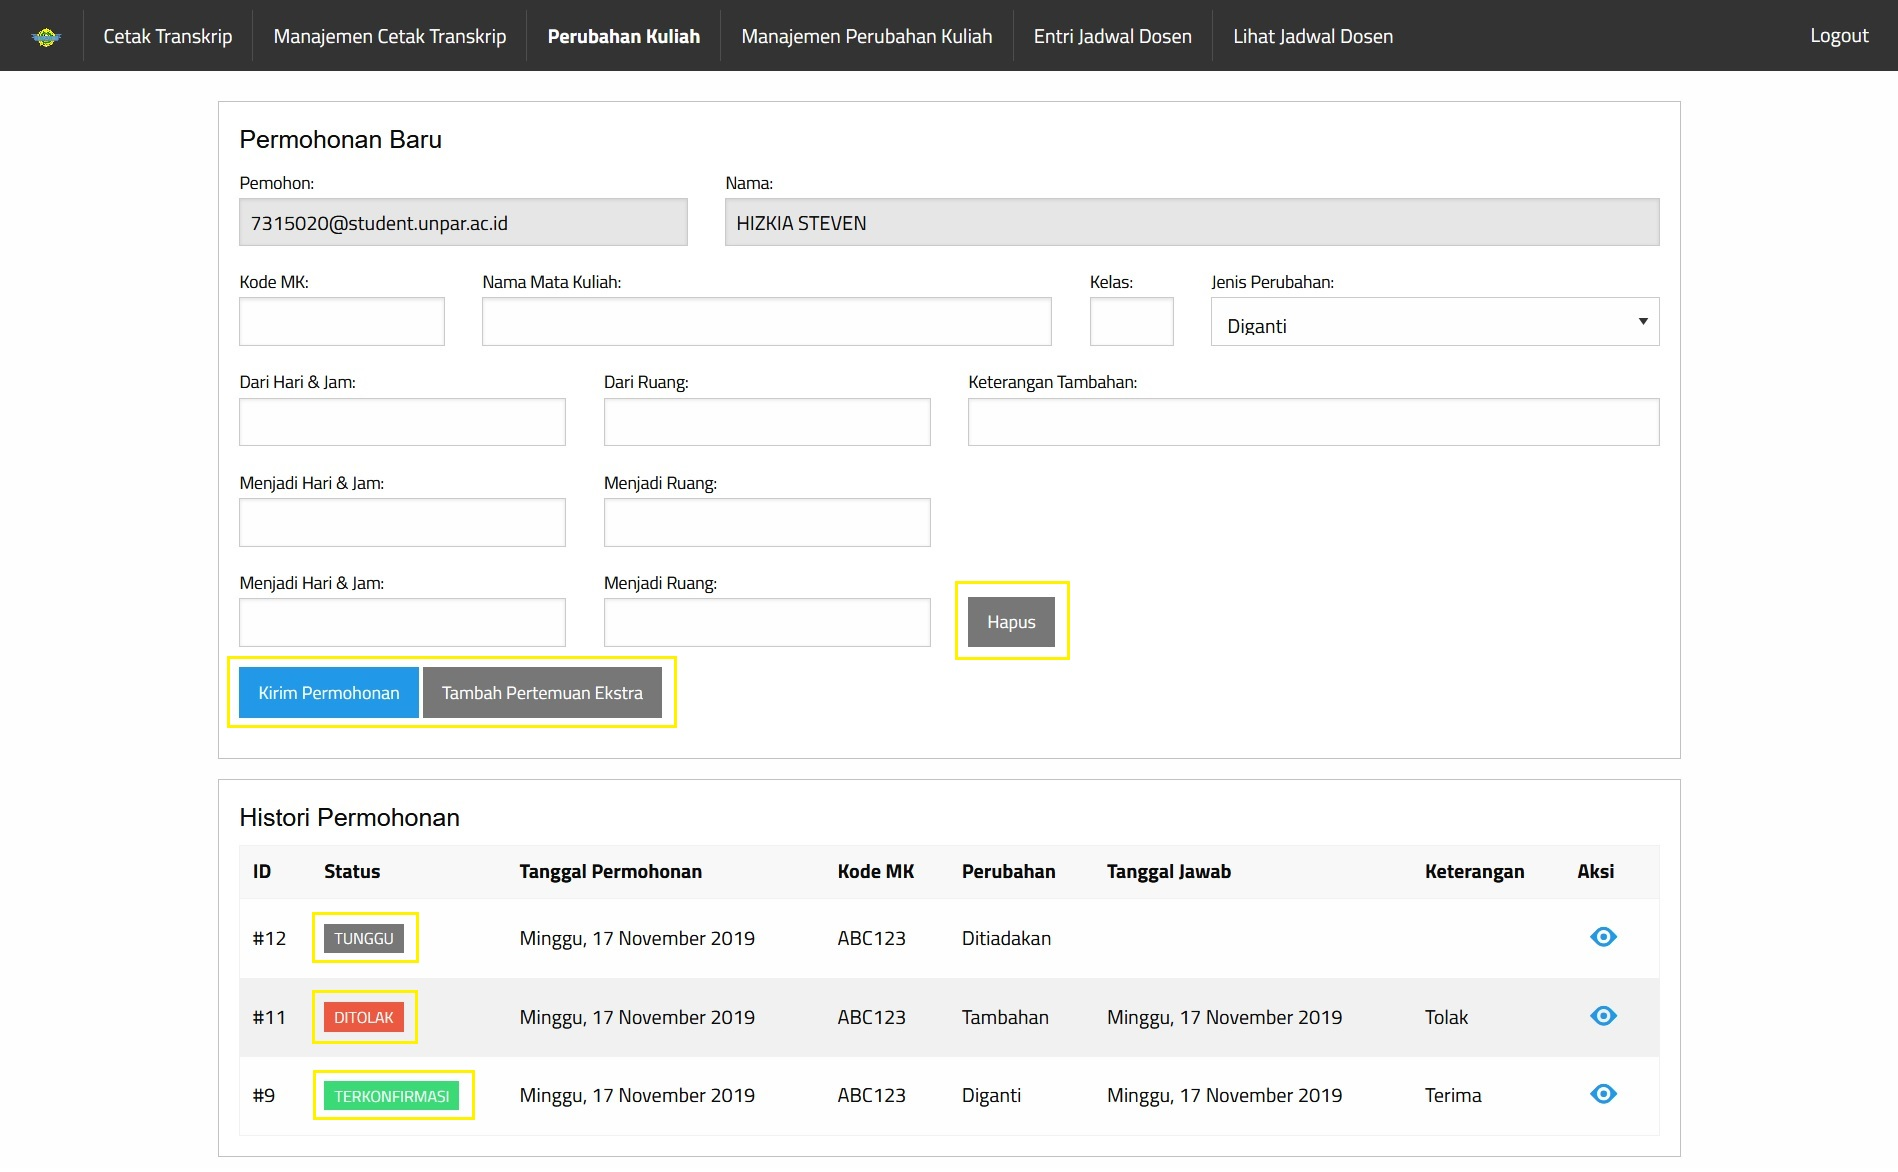
\includegraphics[scale=0.5]{kriteria-sukses-1-4-6-contrast-enchanced-4}  
        \caption[Kriteria Sukses 1.4.6 - Kontras Elemen pada Halaman Perubahan Kuliah]{Kriteria Sukses 1.4.6 - Kontras Elemen pada Halaman Perubahan Kuliah}
        \label{fig:1.4.6_contrast_enchanced_4}  
    \end{figure} 
    Tautan untuk halaman yang bermasalah: 
    
    \url{https://bluetape.azurewebsites.net/PerubahanKuliahRequest}.
    
    \item Halaman manajemen perubahan kuliah: Teks "Terkonfirmasi" di kolom status pada tabel memiliki rasio kontras 1,79:1 terhadap warna latar belakangnya. Teks "Menunggu" di kolom status pada tabel memiliki rasio kontras 1,84:1 terhadap warna latar belakangnya. Teks "Ditolak" di kolom status pada tabel memiliki rasio kontras 3,44:1 terhadap warna latar belakangnya. Teks "Hapus" pada bagian hapus permohonan memiliki rasio kontras 3,47:1 terhadap warna latar belakangnya. Tampilan pada halaman web dapat dilihat pada gambar \ref{fig:1.4.6_contrast_enchanced_5}.
    \begin{figure}[H]
        \centering  
        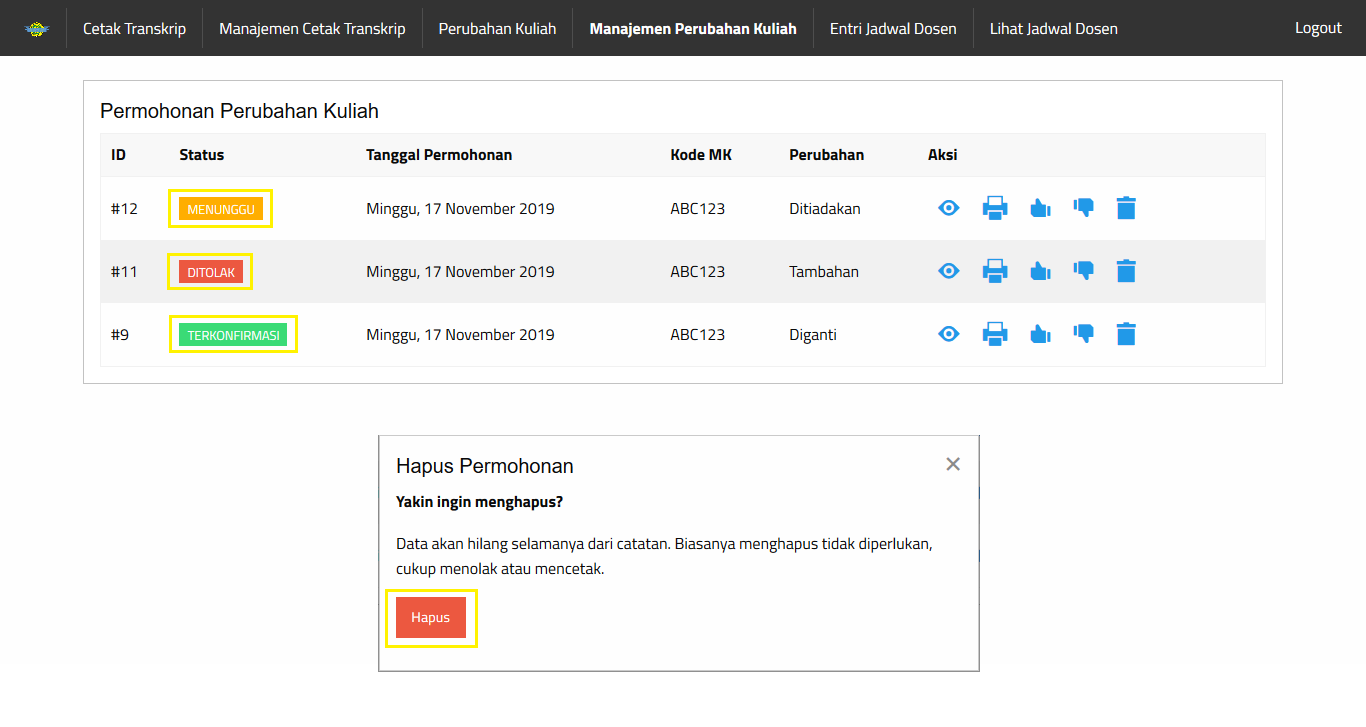
\includegraphics[scale=0.5]{kriteria-sukses-1-4-6-contrast-enchanced-5}  
        \caption[Kriteria Sukses 1.4.6 - Kontras Elemen pada Halaman Manajemen Perubahan Kuliah]{Kriteria Sukses 1.4.6 - Kontras Elemen pada Halaman Manajemen Perubahan Kuliah}
        \label{fig:1.4.6_contrast_enchanced_5}  
    \end{figure} 
    Tautan untuk halaman yang bermasalah: 
    
    \url{https://bluetape.azurewebsites.net/PerubahanKuliahManage}.

    \item Halaman entri jadwal dosen: Teks "Tambah" memiliki rasio kontras 3.09:1 terhadap warna latar belakangnya. Teks "Delete All" memiliki rasio kontras 3.47:1 terhadap warna latar belakangnya. Teks "Ekspor ke XLS" memiliki rasio kontras 3.09:1 terhadap warna latar belakangnya. Teks "Save" pada bagian "Edit Jadwal" memiliki rasio kontras 3.09:1 terhadap warna latar belakangnya. Teks "Delete" memiliki rasio kontras 3.47:1 terhadap warna latar belakangnya. Tampilan pada halaman web dapat dilihat pada gambar \ref{fig:1.4.6_contrast_enchanced_6}.
    \begin{figure}[H]
        \centering  
        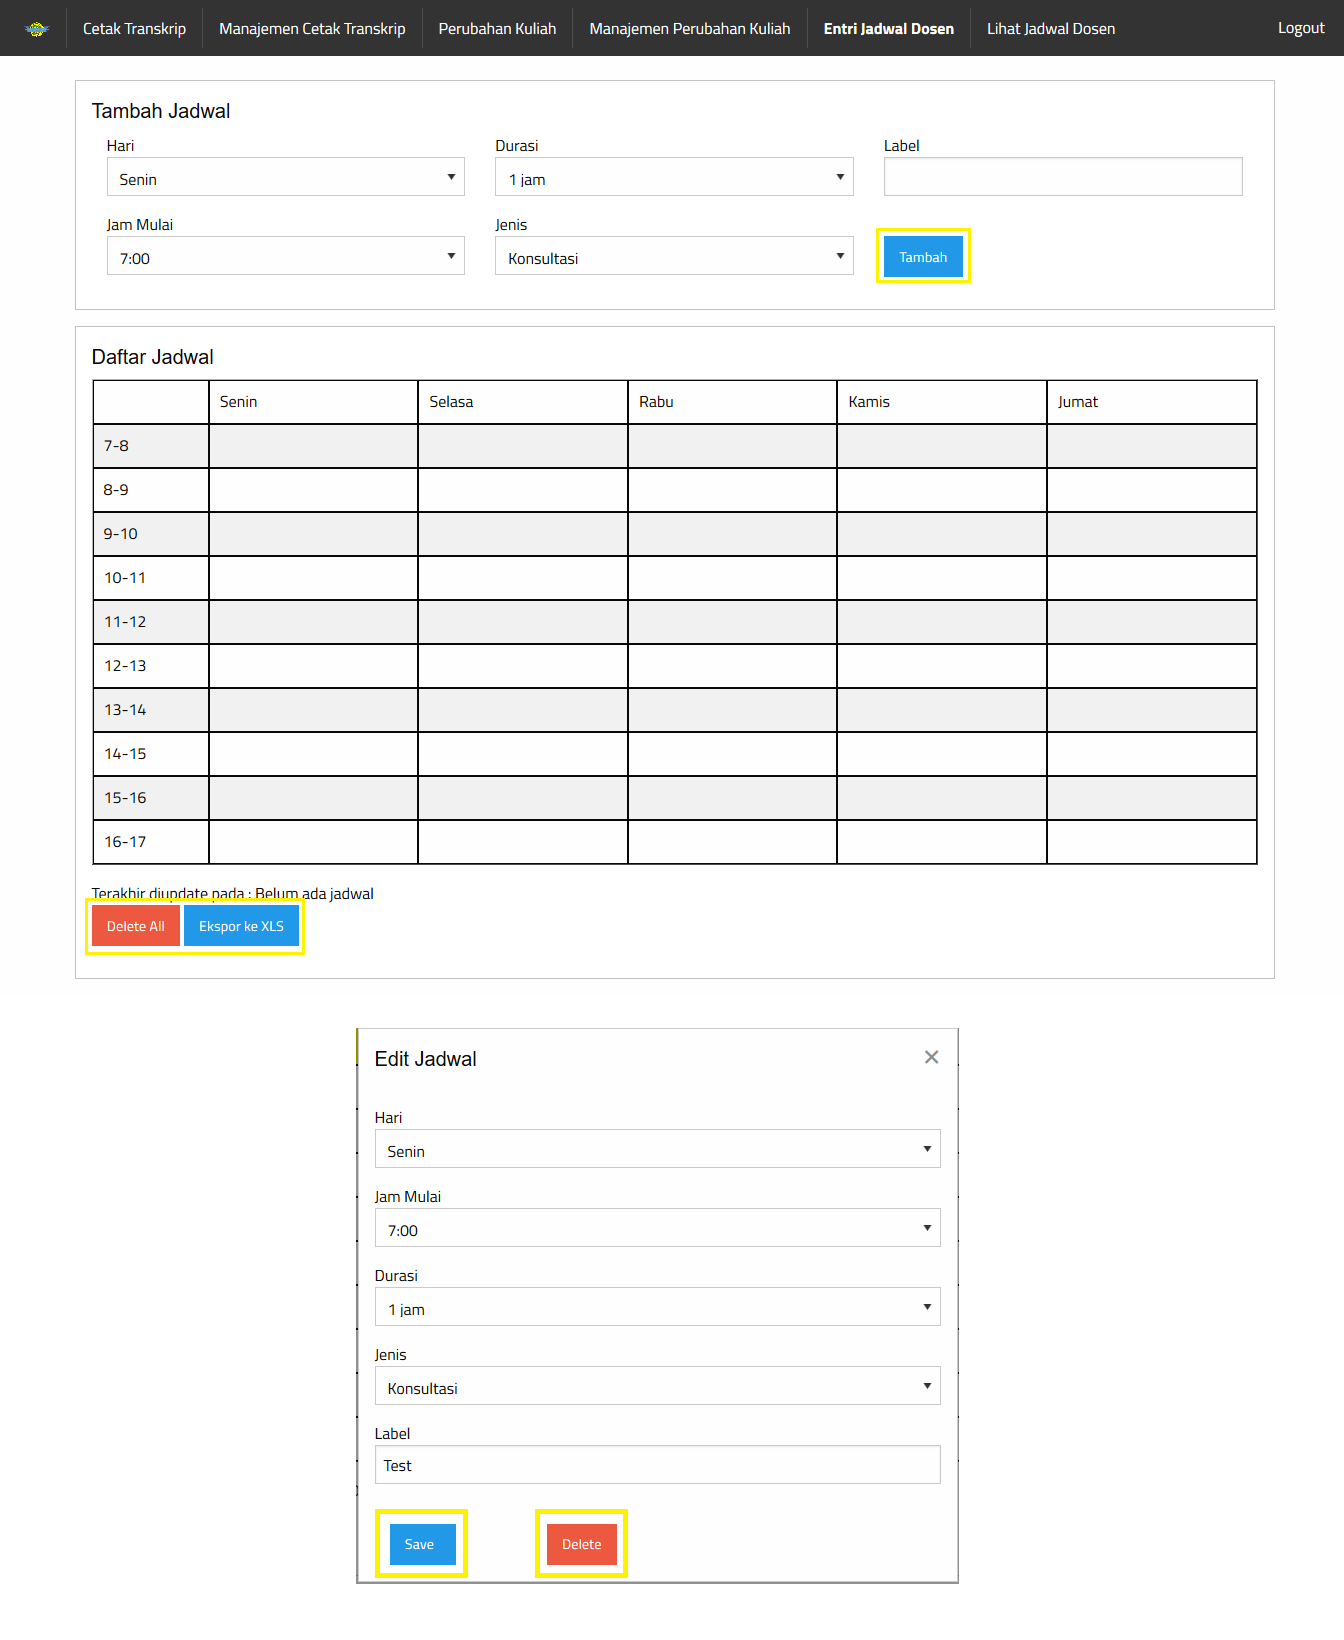
\includegraphics[scale=0.5]{kriteria-sukses-1-4-6-contrast-enchanced-6}  
        \caption[Kriteria Sukses 1.4.6 - Kontras Elemen pada Halaman Entri Jadwal Dosen]{Kriteria Sukses 1.4.6 - Kontras Elemen pada Halaman Entri Jadwal Dosen}
        \label{fig:1.4.6_contrast_enchanced_6}  
    \end{figure} 
    Tautan untuk halaman yang bermasalah: 
    
    \url{https://bluetape.azurewebsites.net/EntriJadwalDosen}.
    
    \item Halaman lihat jadwal dosen: Teks nama dosen di atas tabel yang sedang dipilih pengguna memiliki rasio kontras 2,47:1 terhadap warna latar belakangnya. Teks nama dosen di atas tabel yang sedang tidak dipilih pengguna memiliki rasio kontras 3,06:1 terhadap warna latar belakangnya. Teks "Ekspor ke XLS" memiliki rasio kontras 3.09:1 terhadap warna latar belakangnya. Tampilan pada halaman web dapat dilihat pada gambar \ref{fig:1.4.6_contrast_enchanced_7}.
    \begin{figure}[H]
        \centering  
        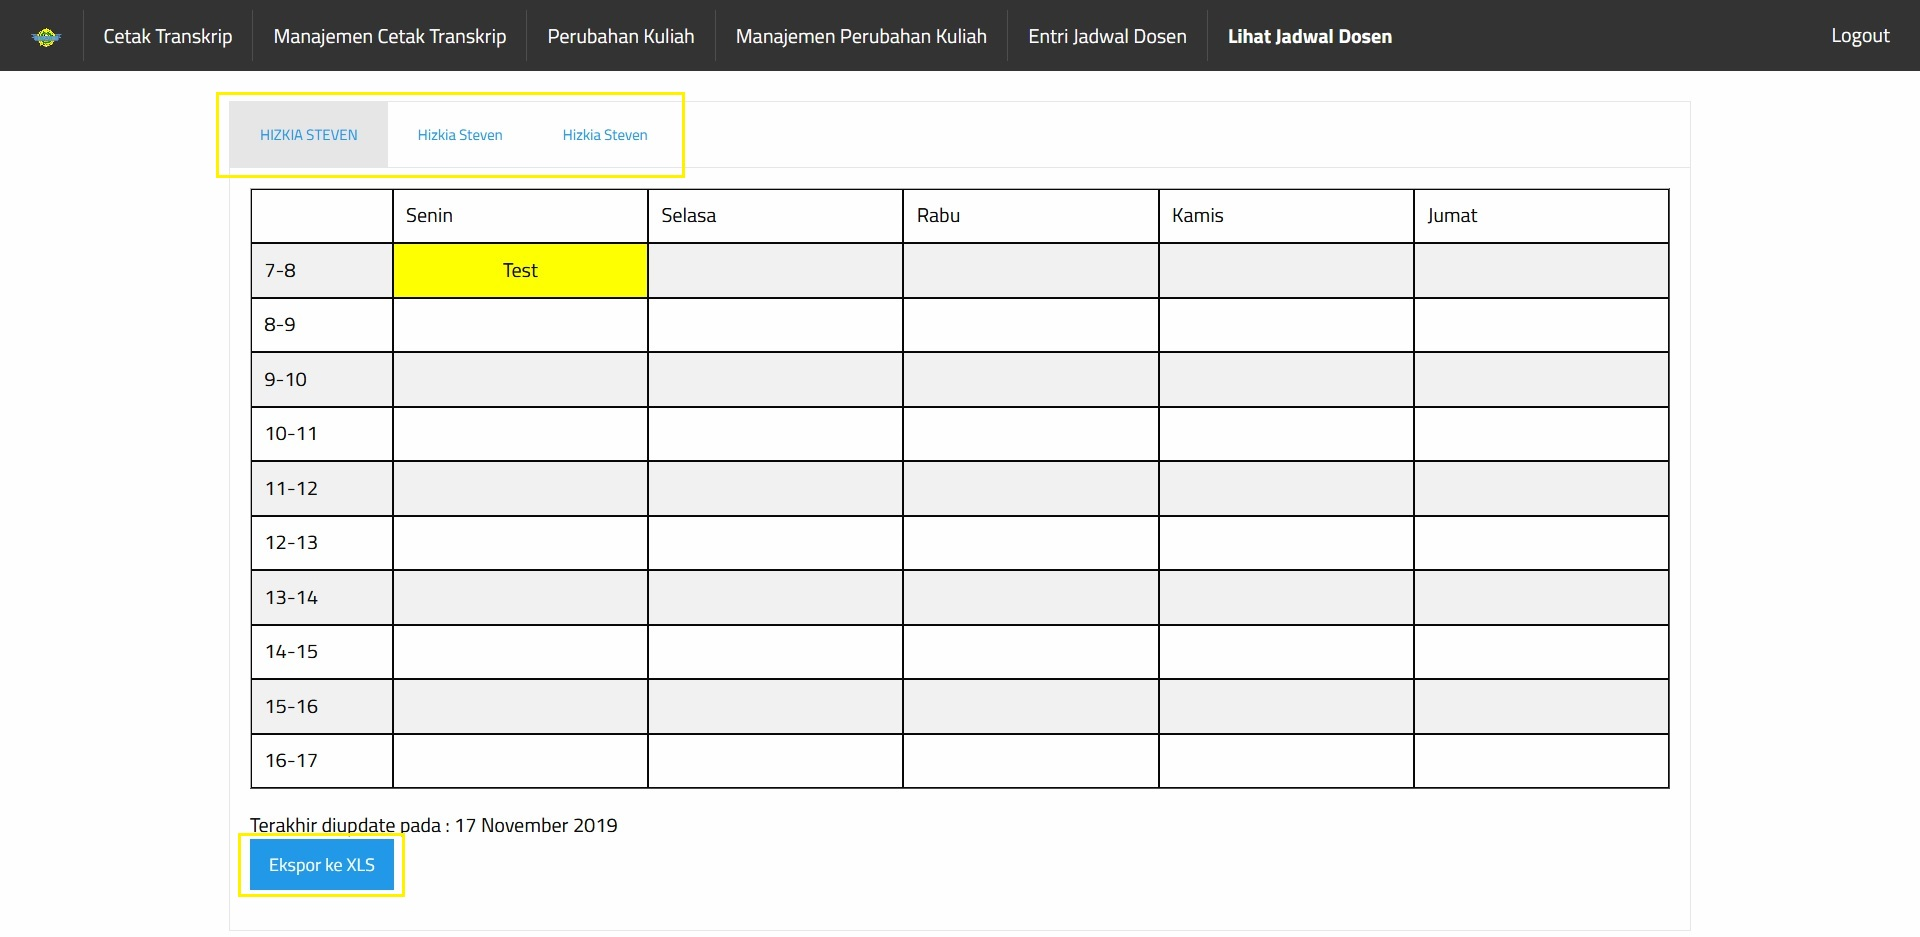
\includegraphics[scale=0.5]{kriteria-sukses-1-4-6-contrast-enchanced-7}  
        \caption[Kriteria Sukses 1.4.6 - Kontras Elemen pada Halaman Lihat Jadwal Dosen]{Kriteria Sukses 1.4.6 - Kontras Elemen pada Halaman Lihat Jadwal Dosen}
        \label{fig:1.4.6_contrast_enchanced_7}  
    \end{figure} 
    Tautan untuk halaman yang bermasalah: 
    
    \url{https://bluetape.azurewebsites.net/LihatJadwalDosen}.
\end{itemize}

\paragraph{Kriteria Sukses 1.4.7 \textit{Low or No Background Audio}}
\label{par:kepatuhan_bluetape_kriteria_sukses_1.4.7}
(Sukses)\\

Kriteria ini sukses dipatuhi karena pada halaman web BlueTape tidak terdapat konten media berbasis waktu.

\paragraph{Kriteria Sukses 1.4.8 \textit{Visual Presentation}}
\label{par:kepatuhan_bluetape_kriteria_sukses_1.4.8}
(Tidak Sukses)\\

Kriteria ini tidak sukses dipatuhi karena pada halaman manajemen cetak transkrip bagian hapus permohonan, teks yang ditampilkan memiliki lebar lebih dari 80 karakter. Tampilan pada halaman web dapat dilihat pada gambar \ref{fig:1.4.8_visual_presentation}.

\begin{figure}[H]
    \centering  
    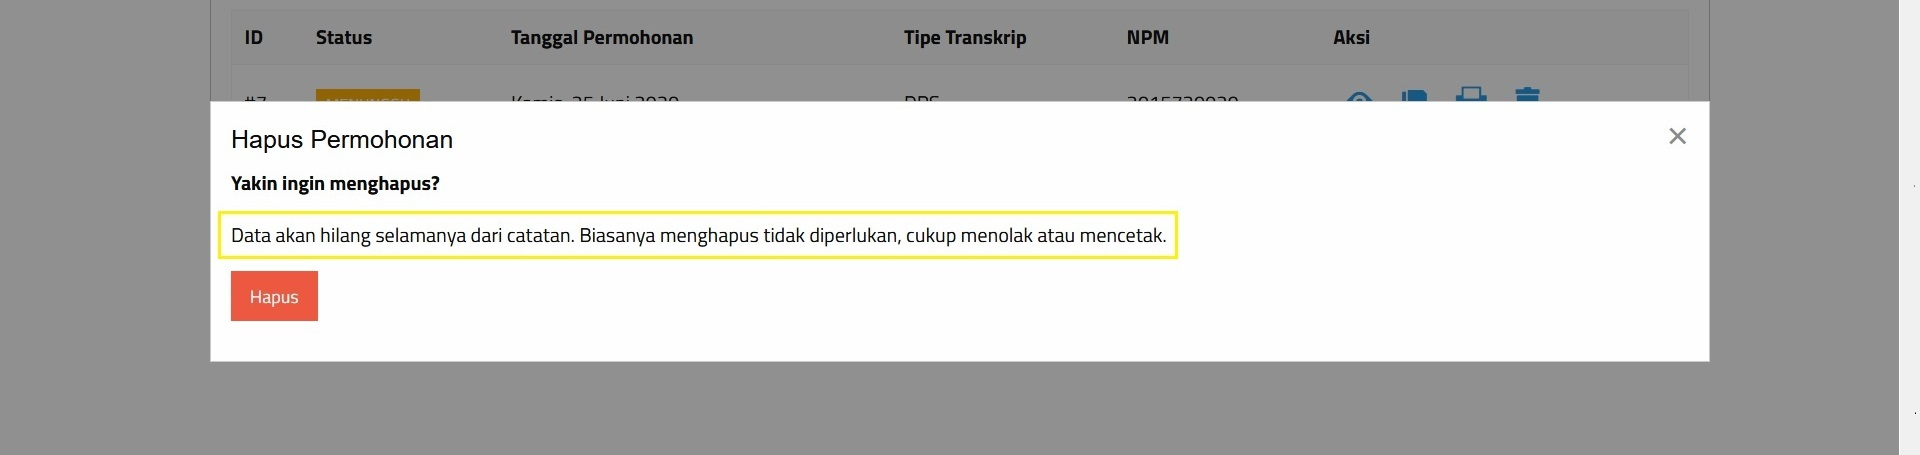
\includegraphics[scale=0.5]{kriteria-sukses-1-4-8-visual-presentation}  
    \caption[Kriteria Sukses 1.4.8 - Teks Terlalu Panjang]{Kriteria Sukses 1.4.8 - Teks Terlalu Panjang}
    \label{fig:1.4.8_visual_presentation}  
\end{figure} 
Tautan untuk halaman yang bermasalah: 

\url{https://bluetape.azurewebsites.net/LihatJadwalDosen}.

\paragraph{Kriteria Sukses 1.4.9 \textit{Images of Text (No Exception)}}
\label{par:kepatuhan_bluetape_kriteria_sukses_1.4.9}
(Sukses)\\

Kriteria ini sukses dipatuhi karena pada halaman web BlueTape tidak terdapat gambar teks selain logo.

\paragraph{Kriteria Sukses 1.4.10 \textit{Reflow}}
\label{par:kepatuhan_bluetape_kriteria_sukses_1.4.10}
(Tidak Sukses)\\

Kriteria ini tidak sukses dipatuhi karena pada halaman web BlueTape, bagian navigasi menu memerlukan \textit{scroll} secara horizontal ketika ditampilkan pada resolusi layar dengan lebar 1280 piksel dan diperbesar hingga 400 persen. Tampilan pada halaman web dapat dilihat pada gambar \ref{fig:1.4.8_visual_presentation}.

\begin{figure}[H]
    \centering  
    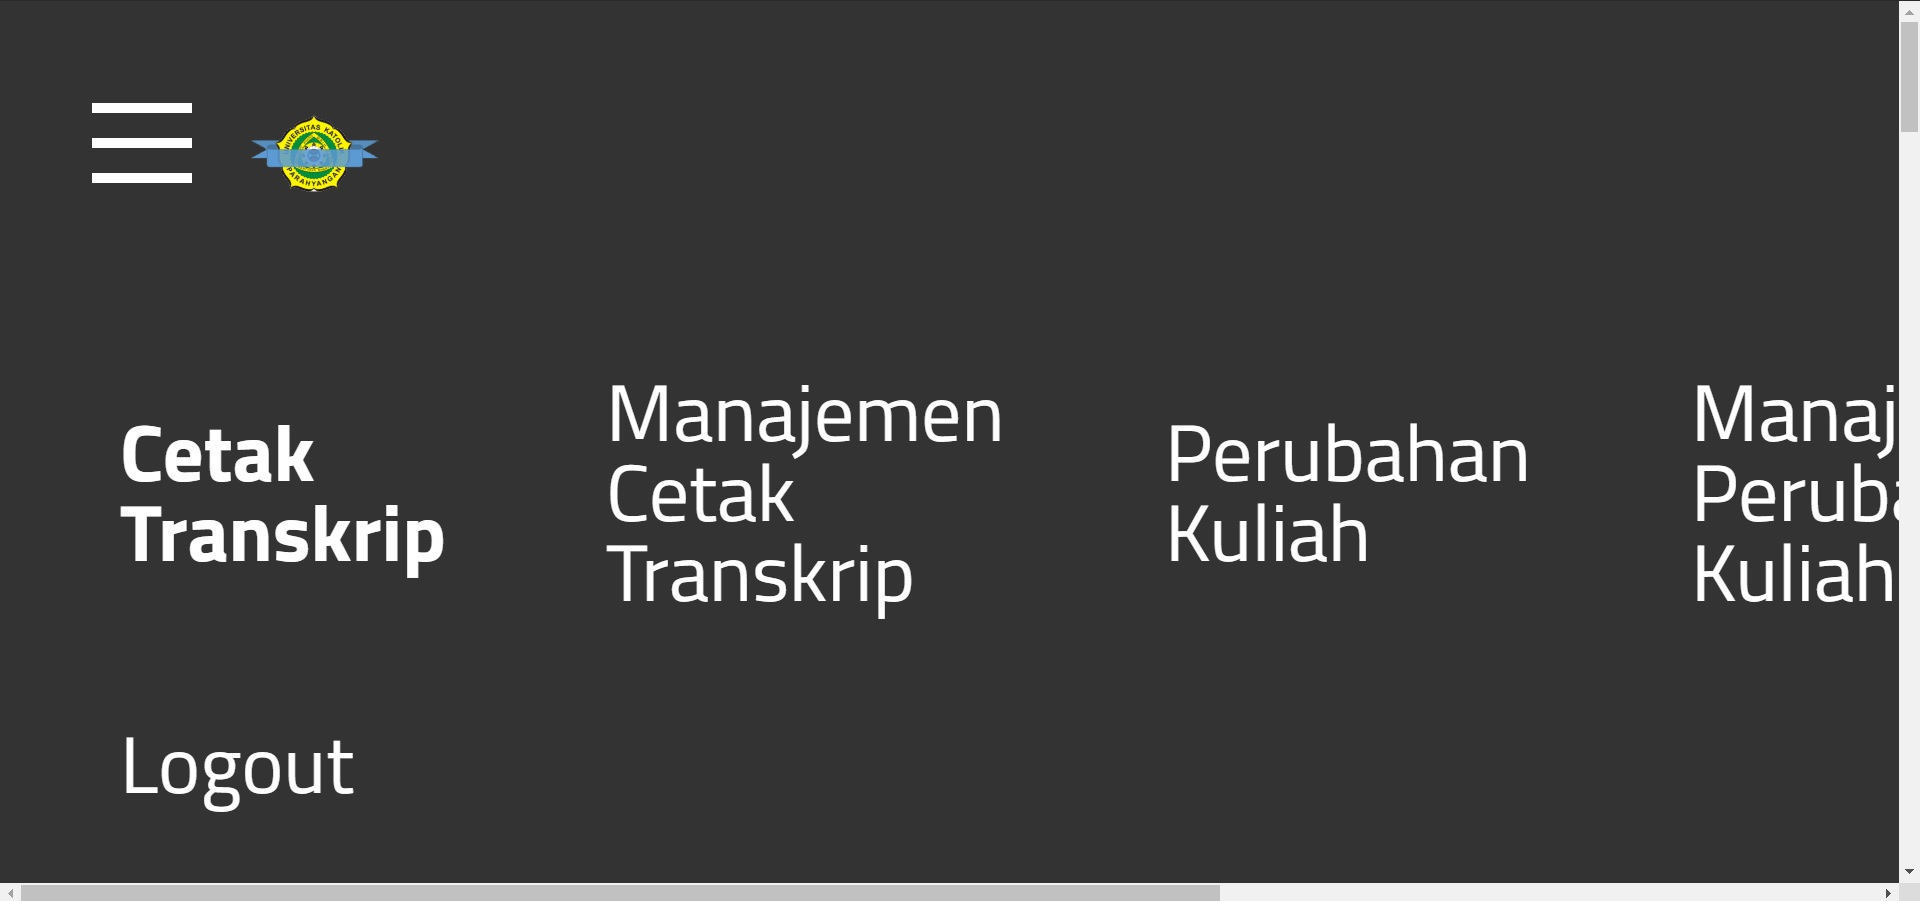
\includegraphics[scale=0.5]{kriteria-sukses-1-4-10-reflow}  
    \caption[Kriteria Sukses 1.4.10 - Horizontal \textit{Scroll} pada Navigasi]{Kriteria Sukses 1.4.10 - Horizontal \textit{Scroll} pada Navigasi}
    \label{fig:1.4.10_reflow}  
\end{figure} 

\paragraph{Kriteria Sukses 1.4.11 \textit{Non-text Contrast}}
\label{par:kepatuhan_bluetape_kriteria_sukses_1.4.11}
(Diabaikan)\\

Kriteria ini diabaikan karena terlalu sulit untuk melakukan pengukuran dan mendapatkan hasilnya. Tampilan pada halaman web dapat dilihat pada gambar \ref{fig:1.4.11_non_text_contrast}.

\begin{figure}[H]
	\centering  
	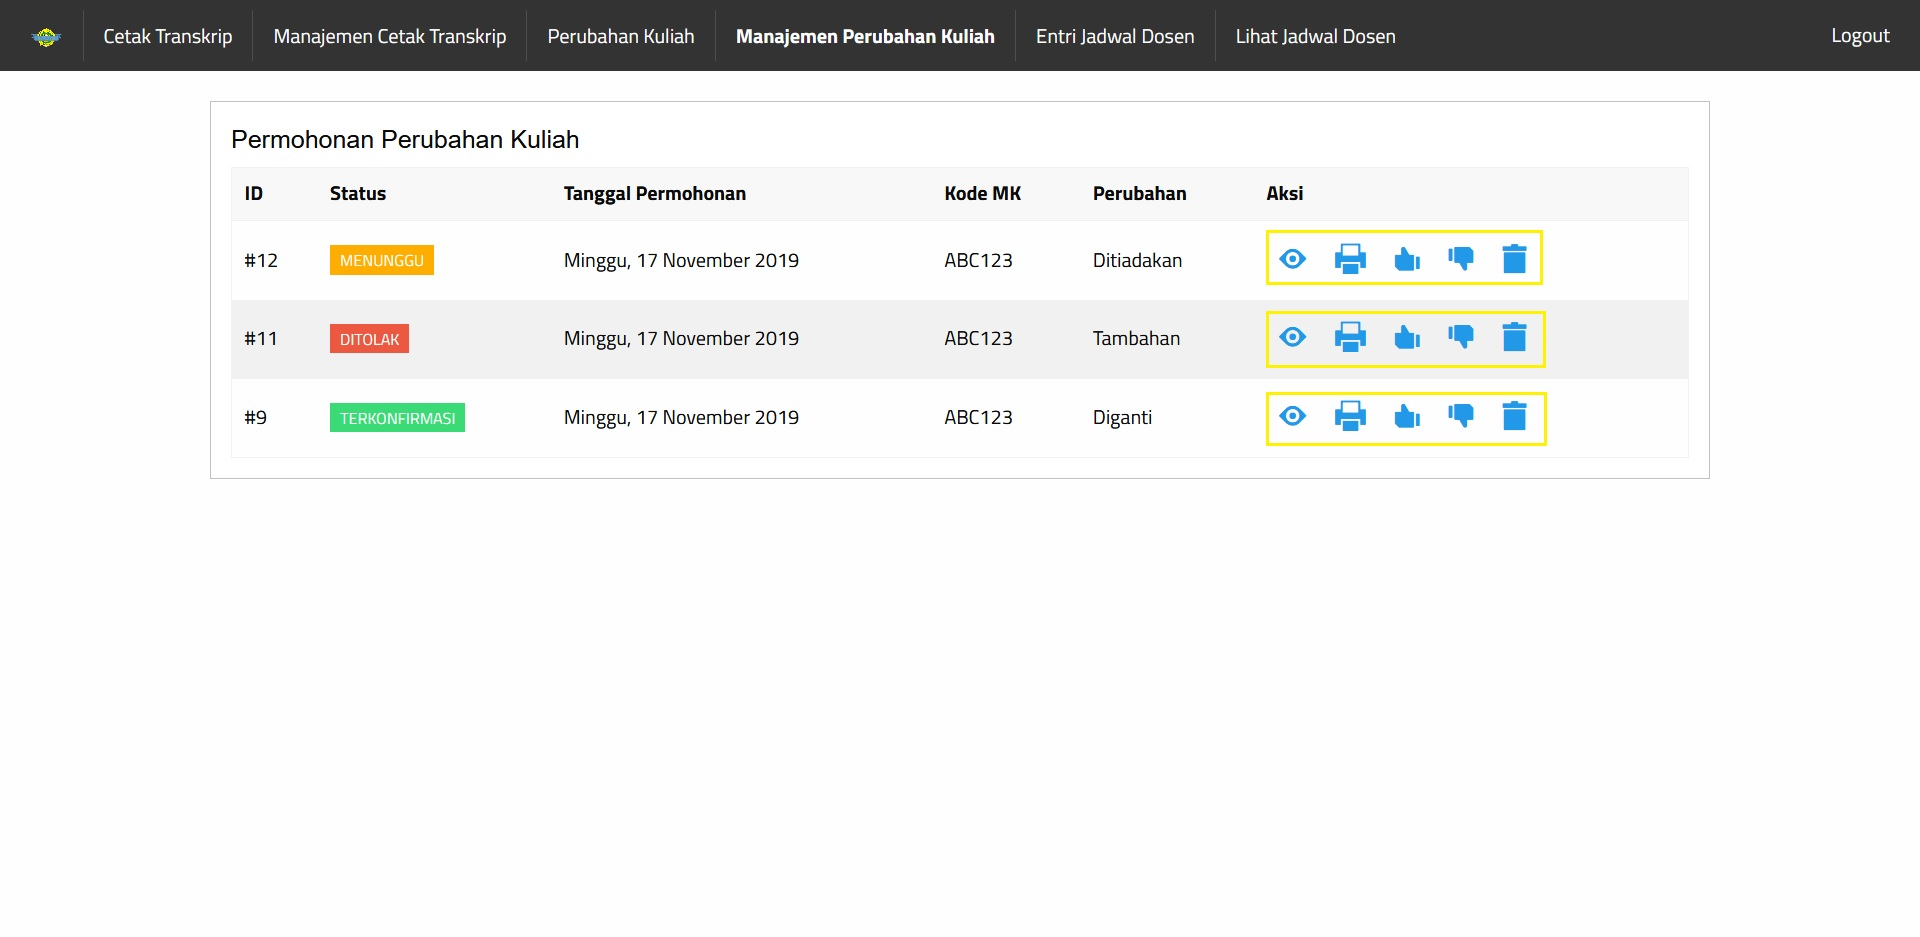
\includegraphics[scale=0.5]{kriteria-sukses-1-4-11-non-text-contrast}  
    \caption[Kriteria Sukses 1.4.11 - Ikon pada Bagian Aksi]{Kriteria Sukses 1.4.11 - Ikon pada Bagian Aksi}
    \label{fig:1.4.11_non_text_contrast}  
\end{figure} 
Contoh tautan untuk halaman yang bermasalah: 

\url{https://bluetape.azurewebsites.net/PerubahanKuliahManage}.

\paragraph{Kriteria Sukses 1.4.12 \textit{Text Spacing}}
\label{par:kepatuhan_bluetape_kriteria_sukses_1.4.12}
(Sukses)\\

Kriteria ini sukses dipatuhi karena penulis sudah melakukan uji coba dengan mengubah beberapa bagian pada halaman perubahan kuliah sesuai kriteria ini dan tidak terjadi masalah. Oleh karena itu, penulis menduga tidak akan ada masalah ketika ukuran-ukuran tertentu diubah pada halaman lain. Tampilan pada halaman web dapat dilihat pada gambar \ref{fig:1.4.12_text_spacing}.

\begin{figure}[H]
	\centering  
	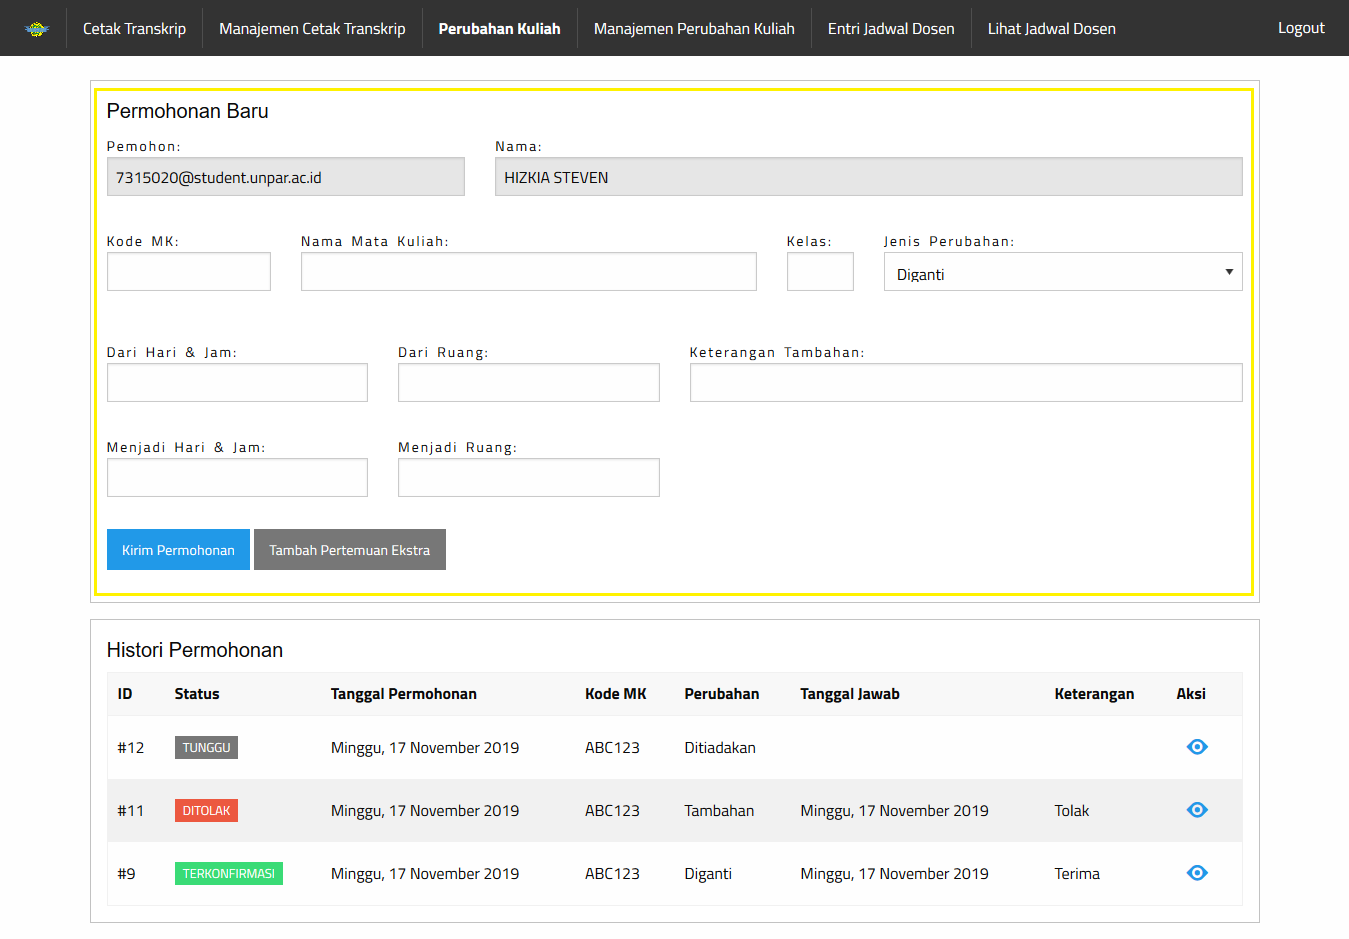
\includegraphics[scale=0.5]{kriteria-sukses-1-4-12-text-spacing}  
    \caption[Kriteria Sukses 1.4.12 - Uji Coba Mengubah Ukuran Elemen]{Kriteria Sukses 1.4.12 - Uji Coba Mengubah Ukuran Elemen}
    \label{fig:1.4.12_text_spacing}  
\end{figure} 

\paragraph{Kriteria Sukses 1.4.13 \textit{Content on Hover or Focus}}
\label{par:kepatuhan_bluetape_kriteria_sukses_1.4.13}
(Sukses)\\

Kriteria ini sukses dipatuhi karena setiap konten tambahan yang muncul sesaat ketika suatu elemen menerima penunjuk kursor atau fokus \textit{keyboard}, konten tambahan tersebut dapat disingkirkan, dapat ditunjuk, dan persisten.

\subsection{\textit{Operable}}
\label{subsec:kepatuhan_bluetape_operable}

\subsubsection{\textit{Keyboard Accessible}}
\label{subsubsec:kepatuhan_bluetape_keyboard_accessible}

\paragraph{Kriteria Sukses 2.1.1 \textit{Keyboard}}
\label{par:kepatuhan_bluetape_kriteria_sukses_2.1.1}
(Tidak Sukses)\\

Kriteria ini tidak sukses dipatuhi karena terdapat fungsionalitas konten yang tidak dapat dioperasikan melalui \textit{keyboard}, antara lain:

\begin{itemize}
    \item Pada bagian navigasi menu, pengguna tidak dapat memilih halaman yang diinginkan. Tampilan pada halaman web dapat dilihat pada gambar \ref{fig:2.1.1_keyboard_1}.
    \begin{figure}[H]
        \centering  
        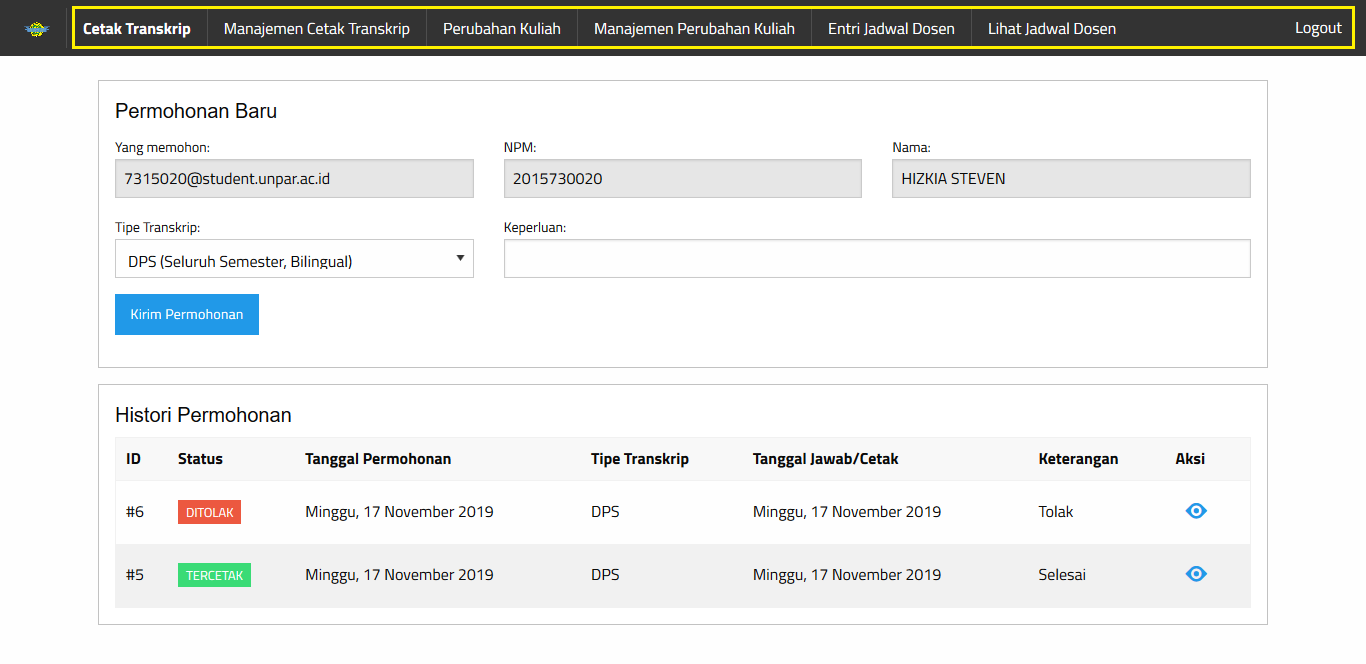
\includegraphics[scale=0.5]{kriteria-sukses-2-1-1-keyboard-1}  
        \caption[Kriteria Sukses 2.1.1 - Penggunaan \textit{Keyboard} pada Menu Navigasi]{Kriteria Sukses 2.1.1 - Penggunaan \textit{Keyboard} pada Menu Navigasi}
        \label{fig:2.1.1_keyboard_1}  
    \end{figure} 

    \item Pada bagian tabel "Daftar Jadwal" di halaman entri jadwal dosen. Tampilan pada halaman web dapat dilihat pada gambar \ref{fig:2.1.1_keyboard_2}.
    \begin{figure}[H]
        \centering  
        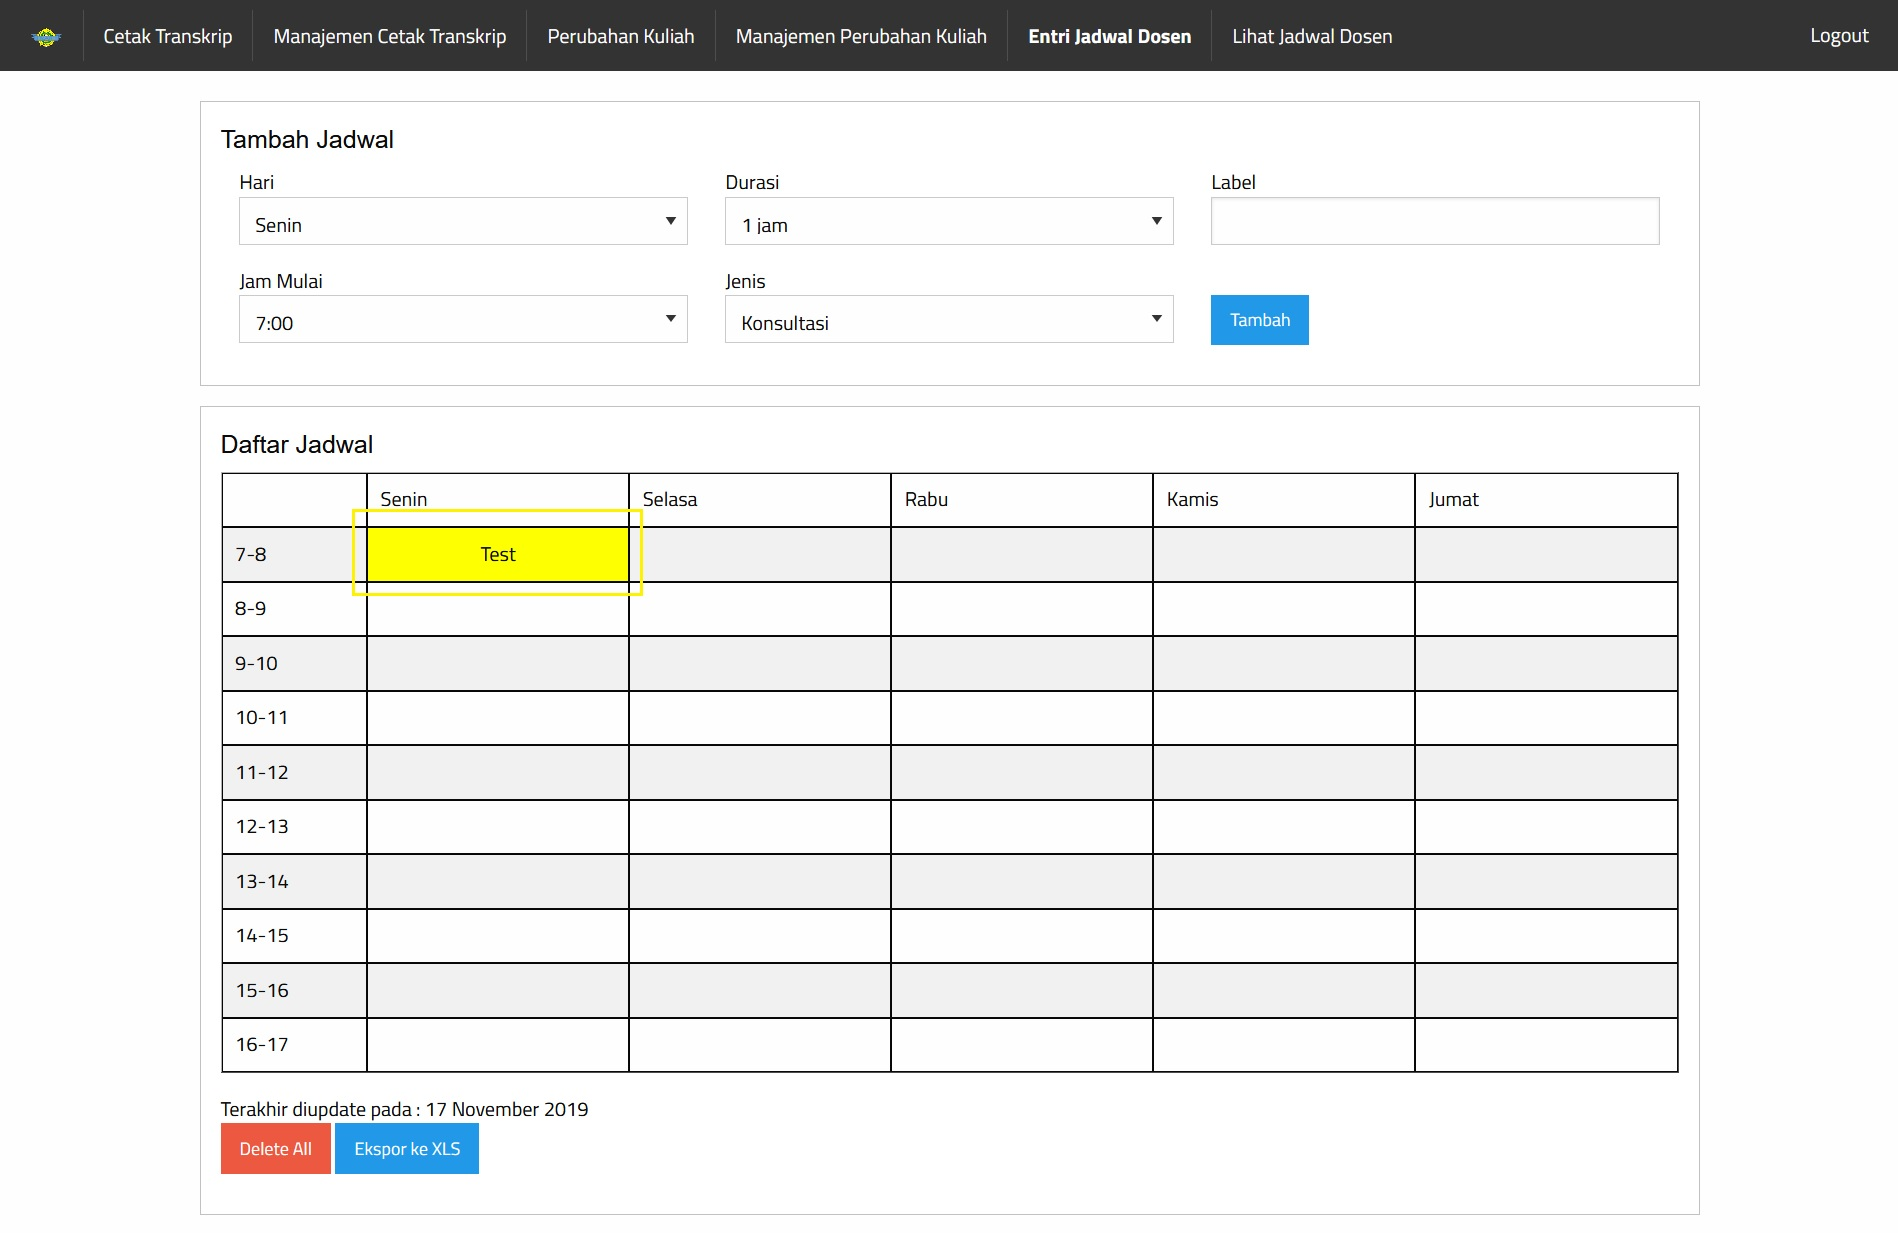
\includegraphics[scale=0.5]{kriteria-sukses-2-1-1-keyboard-2}  
        \caption[Kriteria Sukses 2.1.1 - Penggunaan \textit{Keyboard} pada Halaman Entri Jadwal Dosen]{Kriteria Sukses 2.1.1 - Penggunaan \textit{Keyboard} pada Halaman Entri Jadwal Dosen}
        \label{fig:2.1.1_keyboard_2}  
    \end{figure} 
    Tautan untuk halaman yang bermasalah: 
    
    \url{https://bluetape.azurewebsites.net/EntriJadwalDosen}.
\end{itemize}

\paragraph{Kriteria Sukses 2.1.2 \textit{No Keyboard Trap}}
\label{par:kepatuhan_bluetape_kriteria_sukses_2.1.2}
(Sukses)\\

Kriteria ini sukses dipatuhi karena pengguna dapat bernavigasi dari satu komponen ke komponen lain pada setiap komponen yang dapat dinavigasikan pada halaman web BlueTape dengan menggunakan \textit{keyboard} tanpa terperangkap dalam suatu komponen tertentu.

\paragraph{Kriteria Sukses 2.1.3 \textit{Keyboard (No Exception)}}
\label{par:kepatuhan_bluetape_kriteria_sukses_2.1.3}
(Tidak Sukses)\\

Kriteria ini tidak sukses dipatuhi karena terdapat fungsionalitas konten yang tidak dapat dioperasikan melalui \textit{keyboard}, antara lain:

\begin{itemize}
    \item Pada bagian navigasi menu, pengguna tidak dapat memilih halaman yang diinginkan. Tampilan pada halaman web dapat dilihat pada gambar \ref{fig:2.1.3_keyboard_no_exception_1}.
    \begin{figure}[H]
        \centering  
        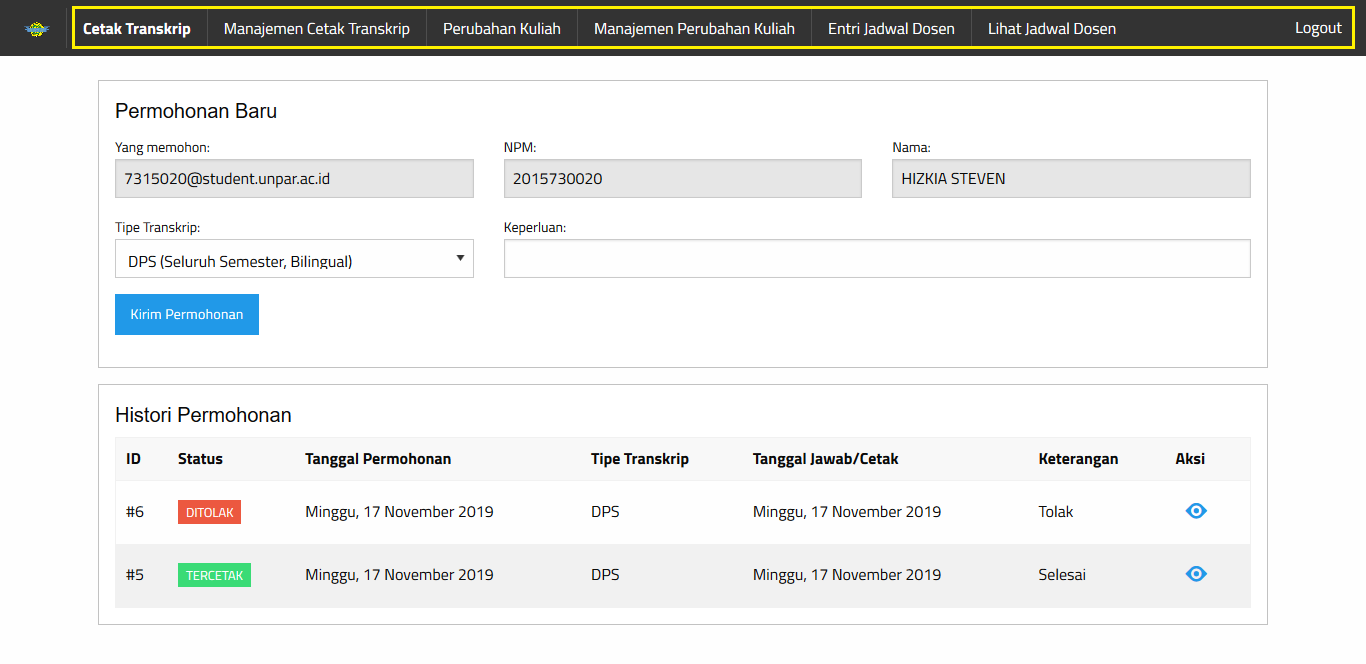
\includegraphics[scale=0.5]{kriteria-sukses-2-1-3-keyboard-no-exception-1}  
        \caption[Kriteria Sukses 2.1.3 - Penggunaan \textit{Keyboard} pada Menu Navigasi]{Kriteria Sukses 2.1.3 - Penggunaan \textit{Keyboard} pada Menu Navigasi}
        \label{fig:2.1.3_keyboard_no_exception_1}  
    \end{figure} 

    \item Pada bagian tabel "Daftar Jadwal" di halaman entri jadwal dosen. Tampilan pada halaman web dapat dilihat pada gambar \ref{fig:2.1.3_keyboard_no_exception_2}.
    \begin{figure}[H]
        \centering  
        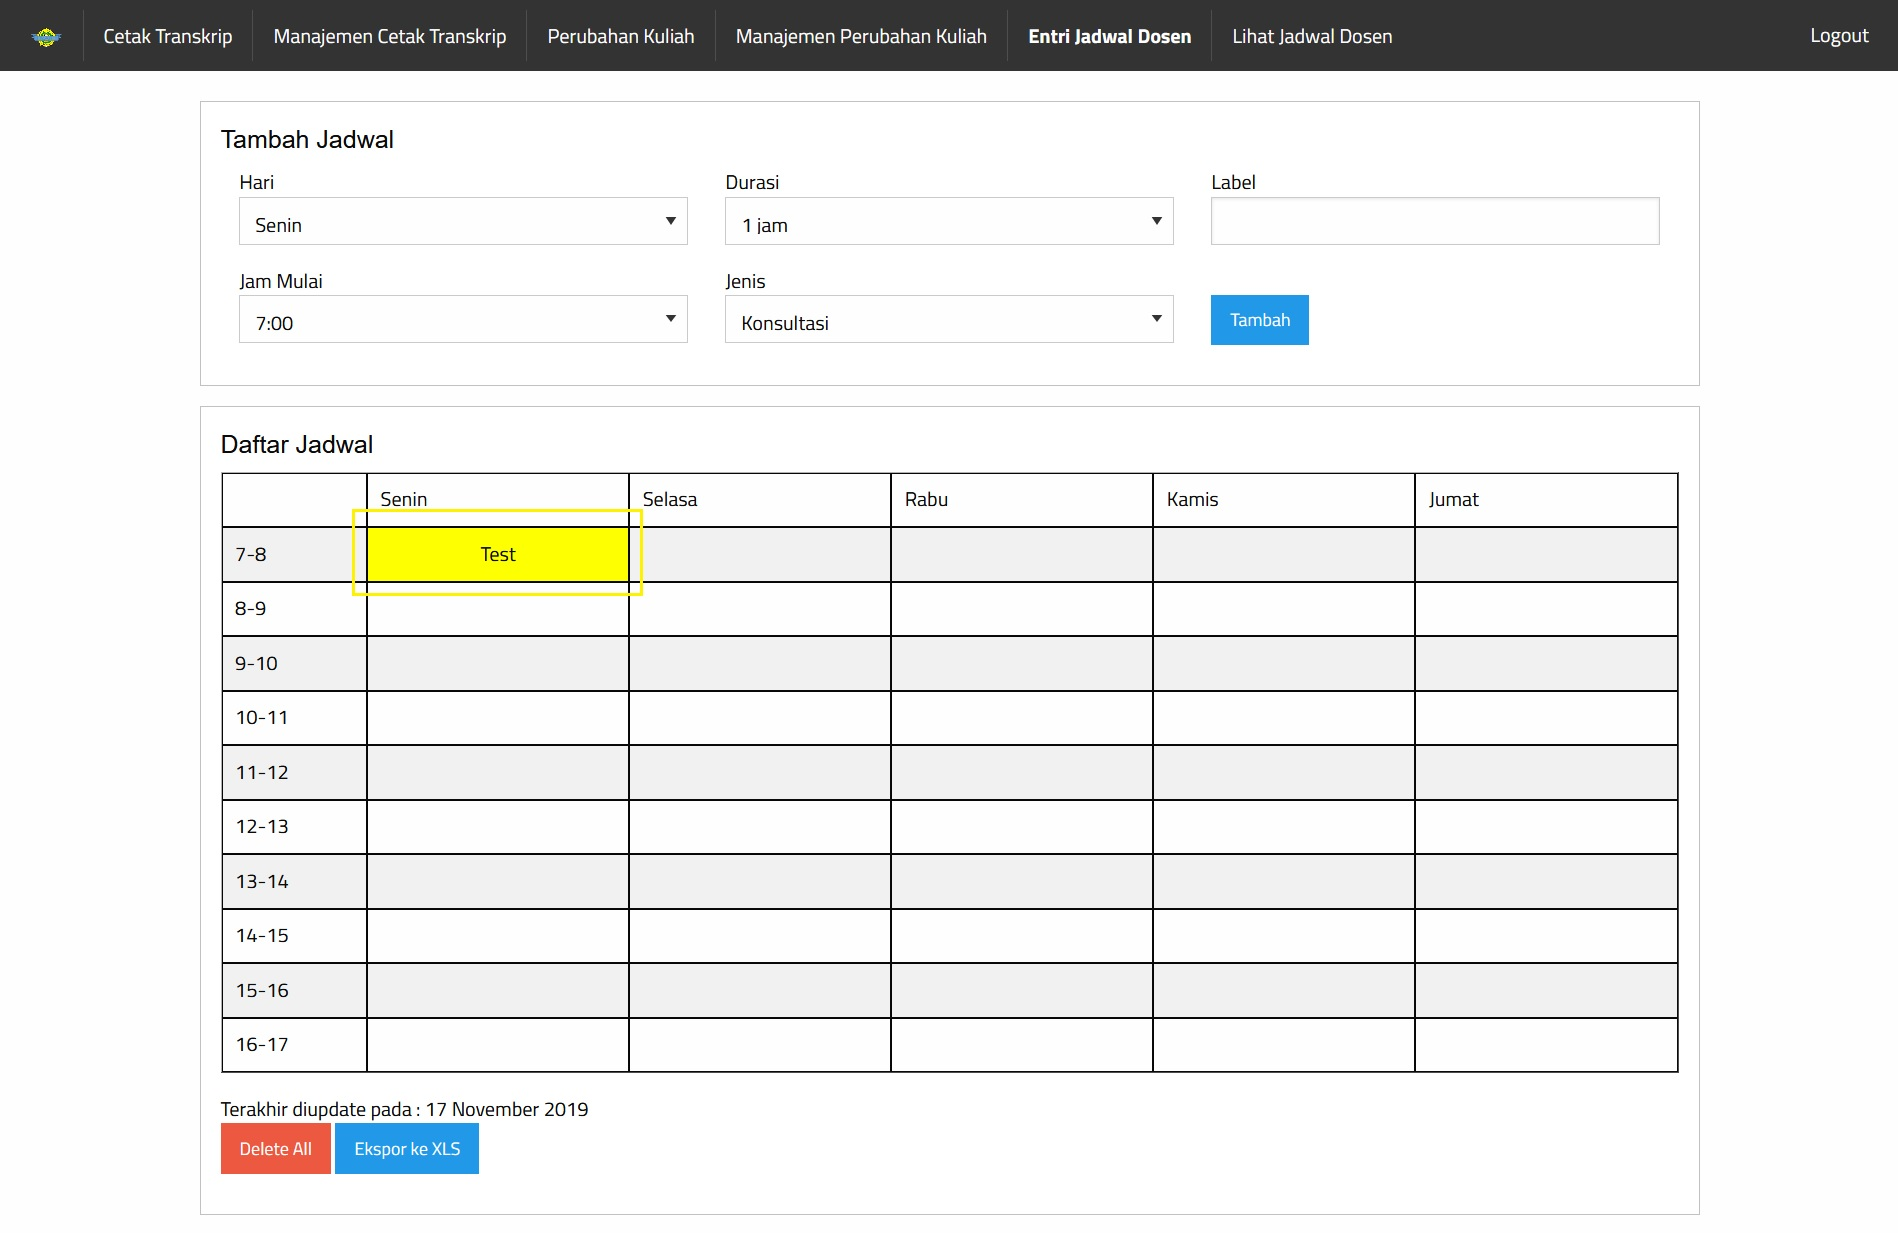
\includegraphics[scale=0.5]{kriteria-sukses-2-1-3-keyboard-no-exception-2}  
        \caption[Kriteria Sukses 2.1.3 - Penggunaan \textit{Keyboard} pada Halaman Entri Jadwal Dosen]{Kriteria Sukses 2.1.3 - Penggunaan \textit{Keyboard} pada Halaman Entri Jadwal Dosen}
        \label{fig:2.1.3_keyboard_no_exception_2}  
    \end{figure} 
    Tautan untuk halaman yang bermasalah: 
    
    \url{https://bluetape.azurewebsites.net/EntriJadwalDosen}.
\end{itemize}

\paragraph{Kriteria Sukses 2.1.4 \textit{Character Key Shortcuts}}
\label{par:kepatuhan_bluetape_kriteria_sukses_2.1.4}
(Sukses)\\

Kriteria ini sukses dipatuhi karena pada halaman web BlueTape tidak terdapat pintasan \textit{keyboard} untuk konten yang disajikan.

\subsubsection{\textit{Enough Time}}
\label{subsubsec:kepatuhan_bluetape_enough_time}

\paragraph{Kriteria Sukses 2.2.1 \textit{Timing Adjustable}}
\label{par:kepatuhan_bluetape_kriteria_sukses_2.2.1}
(Sukses)\\

Kriteria ini sukses dipatuhi karena pada halaman web BlueTape tidak terdapat batas waktu bagi pengguna untuk membaca dan memanfaatkan konten.

\paragraph{Kriteria Sukses 2.2.2 \textit{Pause, Stop, Hide}}
\label{par:kepatuhan_bluetape_kriteria_sukses_2.2.2}
(Sukses)\\

Kriteria ini sukses dipatuhi karena pada halaman web BlueTape tidak terdapat konten yang bergerak, berkelip, bergulir, ataupun diperbarui otomatis.

\paragraph{Kriteria Sukses 2.2.3 \textit{No Timing}}
\label{par:kepatuhan_bluetape_kriteria_sukses_2.2.3}
(Sukses)\\

Kriteria ini sukses dipatuhi karena pada halaman web BlueTape tidak terdapat batas waktu bagi pengguna untuk membaca dan memanfaatkan konten.

\paragraph{Kriteria Sukses 2.2.4 \textit{Interruptions}}
\label{par:kepatuhan_bluetape_kriteria_sukses_2.2.4}
(Sukses)\\

Kriteria ini sukses dipatuhi karena setiap interupsi pada halaman web BlueTape dapat ditunda atau dihentikan oleh pengguna.

\paragraph{Kriteria Sukses 2.2.5 \textit{Re-authenticating}}
\label{par:kepatuhan_bluetape_kriteria_sukses_2.2.5}
(Tidak Sukses)\\

Kriteria ini tidak sukses dipatuhi karena ketika pengguna akan mengirim data dan sesi autentikasi berakhir, pengguna kehilangan data tersebut setelah melakukan autentikasi ulang.

\paragraph{Kriteria Sukses 2.2.6 \textit{Timeouts}}
\label{par:kepatuhan_bluetape_kriteria_sukses_2.2.6}
(Tidak Sukses)\\

Kriteria ini tidak sukses dipatuhi karena tidak terdapat peringatan untuk pengguna ketika sesi autentikasi akan berakhir yang dapat menyebabkan kehilangan data. Data pengguna tidak disimpan untuk bertahan lebih dari 20 jam ketika pengguna tidak melakukan tindakan apa pun. Pada potongan kode \ref{lst:2.2.6_sesi_autentikasi} ditunjukkan bahwa sesi auntentikasi pengguna hanya bertahan selama 2 jam saja ketika pengguna tidak melakukan tindakan apa pun.

\begin{lstlisting}[frame=single, label={lst:2.2.6_sesi_autentikasi}, language=PHP, caption=Kriteria Sukses 2.2.6 - Sesi Autentikasi]
    $config['sess_cookie_name'] = 'ci_session';
    $config['sess_expiration'] = 7200;
    $config['sess_save_path'] = NULL;
\end{lstlisting}

\subsubsection{\textit{Seizures and Physical Reactions}}
\label{subsubsec:kepatuhan_bluetape_seizures_and_physical_reactions}

\paragraph{Kriteria Sukses 2.3.1 \textit{Three Flashes or Below Threshold}}
\label{par:kepatuhan_bluetape_kriteria_sukses_2.3.1}
(Sukses)\\

Kriteria ini sukses dipatuhi karena pada halaman web BlueTape tidak terdapat konten yang berkelip.

\paragraph{Kriteria Sukses 2.3.2 \textit{Three Flashes}}
\label{par:kepatuhan_bluetape_kriteria_sukses_2.3.2}
(Sukses)\\

Kriteria ini sukses dipatuhi karena pada halaman web BlueTape tidak terdapat konten yang berkelip.

\paragraph{Kriteria Sukses 2.3.3 \textit{Animation from Interactions}}
\label{par:kepatuhan_bluetape_kriteria_sukses_2.3.3}
(Sukses)\\

Kriteria ini sukses dipatuhi karena pada halaman web BlueTape tidak terdapat animasi gerak pada konten yang disajikan ketika pengguna melakukan interaksi dengan komponen-komponen yang ada.

\subsubsection{\textit{Navigable}}
\label{subsubsec:kepatuhan_bluetape_navigable}

\paragraph{Kriteria Sukses 2.4.1 \textit{Bypass Blocks}}
\label{par:kepatuhan_bluetape_kriteria_sukses_2.4.1}
(Tidak Sukses)\\

Kriteria ini tidak sukses dipatuhi karena pada halaman web BlueTape tidak tersedia mekanisme untuk melompati beberapa area konten yang berulang pada beberapa halaman web.

\paragraph{Kriteria Sukses 2.4.2 \textit{Page Titled}}
\label{par:kepatuhan_bluetape_kriteria_sukses_2.4.2}
(Sukses)\\

Kriteria ini sukses dipatuhi karena setiap halaman web BlueTape memiliki judul yang dapat menjelaskan topik atau tujuan dari halaman yang bersangkutan.

\paragraph{Kriteria Sukses 2.4.3 \textit{Focus Order}}
\label{par:kepatuhan_bluetape_kriteria_sukses_2.4.3}
(Sukses)\\

Kriteria ini sukses dipatuhi karena setiap halaman web BlueTape memiliki elemen dengan urutan fokus yang benar. 

\paragraph{Kriteria Sukses 2.4.4 \textit{Link Purpose (In Context)}}
\label{par:kepatuhan_bluetape_kriteria_sukses_2.4.4}
(Tidak Sukses)\\

Kriteria ini tidak sukses dipatuhi karena pada halaman cetak transkrip, manajemen cetak transkrip, perubahan kuliah, dan manajemen perubahan kuliah terdapat tautan yang berisi konten bukan teks dan tidak terdapat teks yang dapat menjelaskan tujuan tautan tersebut. Kesalahan dapat dilihat pada potongan kode \ref{lst:2.4.4_tautan_tanpa_keterangan}. Tampilan pada halaman web dapat dilihat pada gambar \ref{fig:2.4.4_link_purpose_in_context}.

\begin{lstlisting}[frame=single, label={lst:2.4.4_tautan_tanpa_keterangan}, language=HTML, caption=Kriteria Sukses 2.4.4 - Tautan Tanpa Keterangan]
        </div>
        <a data-open="detail6">
            <i class="fi-eye"></i>
        </a>
    </td>
\end{lstlisting}

\begin{figure}[H]
	\centering  
	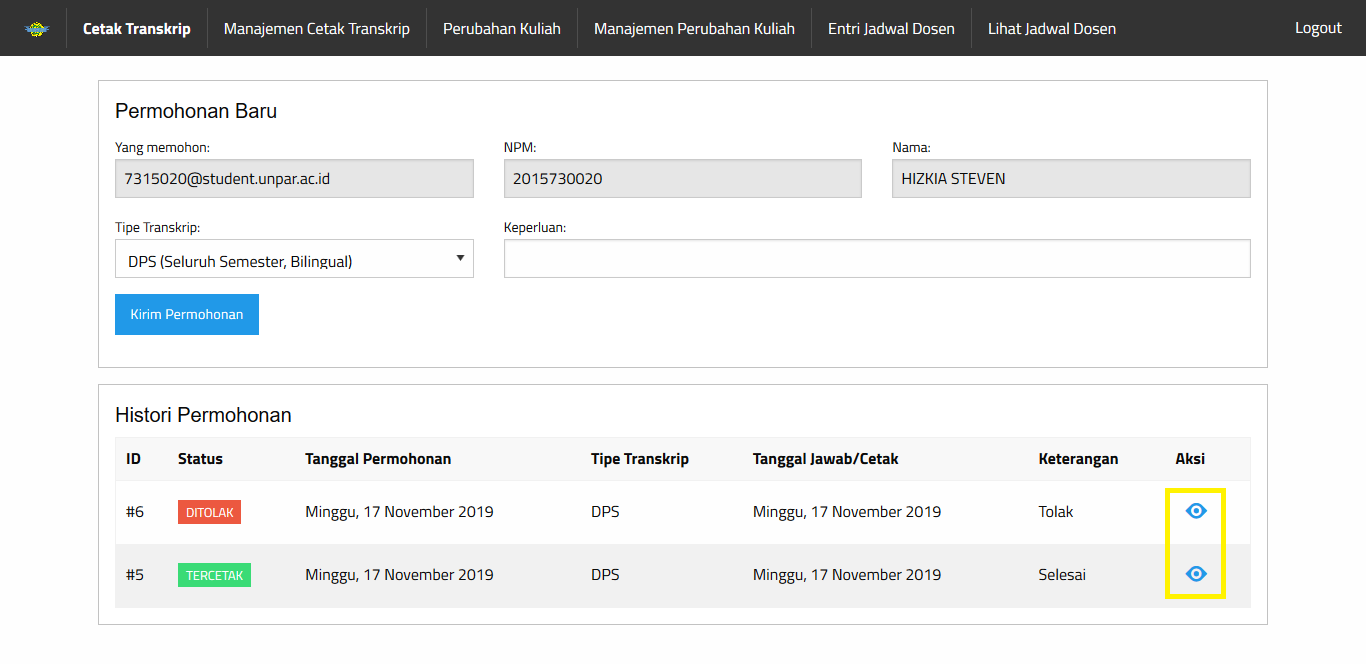
\includegraphics[scale=0.5]{kriteria-sukses-2-4-4-link-purpose-in-context}  
    \caption[Kriteria Sukses 2.4.4 - Tautan Tanpa Keterangan]{Kriteria Sukses 2.4.4 - Tautan Tanpa Keterangan}
    \label{fig:2.4.4_link_purpose_in_context}  
\end{figure} 
Contoh tautan untuk halaman yang bermasalah: 

\url{https://bluetape.azurewebsites.net/TranskripRequest}.

\paragraph{Kriteria Sukses 2.4.5 \textit{Multiple Ways}}
\label{par:kepatuhan_bluetape_kriteria_sukses_2.4.5}
(Tidak Sukses)\\

Kriteria ini tidak sukses dipatuhi karena pada halaman web BlueTape hanya tersedia satu cara untuk menemukan suatu halaman web dalam sekumpulan halaman web yang tersedia, yaitu melalui menu navigasi. Tampilan pada halaman web dapat dilihat pada gambar \ref{fig:2.4.5_multiple_ways}.

\begin{figure}[H]
	\centering  
	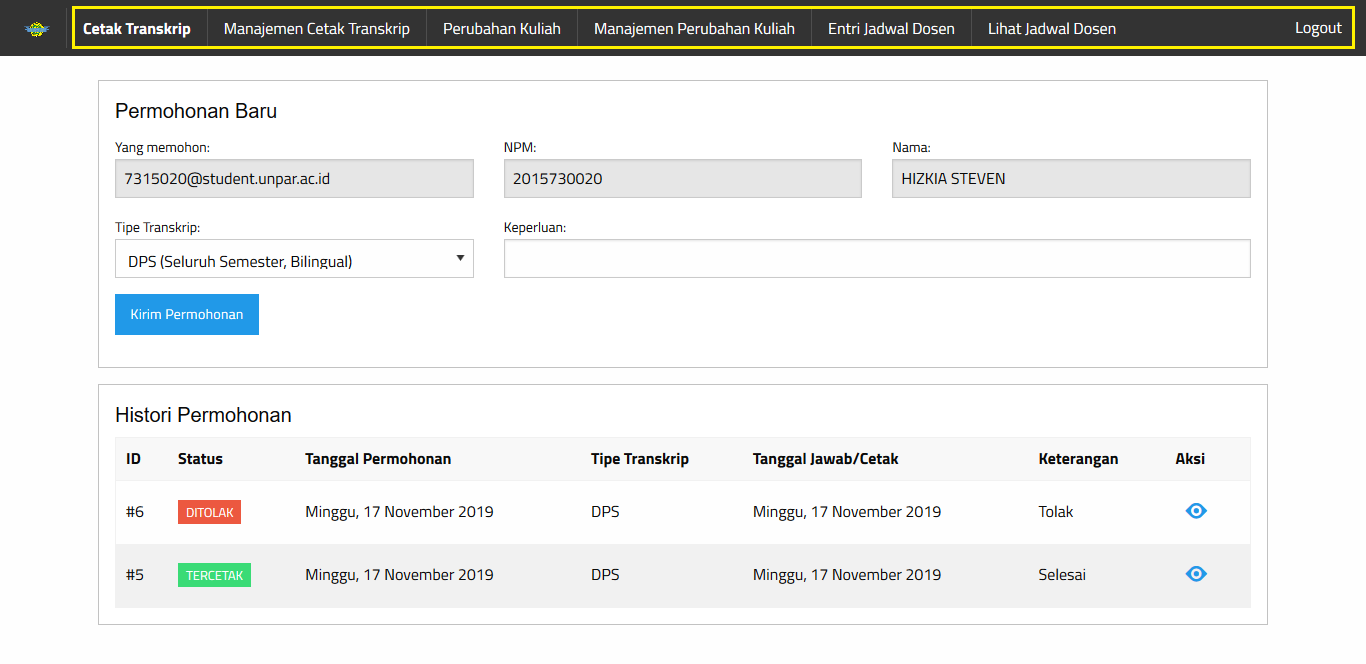
\includegraphics[scale=0.5]{kriteria-sukses-2-4-5-multiple-ways}  
    \caption[Kriteria Sukses 2.4.5 - Menemukan Halaman Web pada Navigasi]{Kriteria Sukses 2.4.5 - Menemukan Halaman Web pada Navigasi}
    \label{fig:2.4.5_multiple_ways}  
\end{figure}

\paragraph{Kriteria Sukses 2.4.6 \textit{Headings and Labels}}
\label{par:kepatuhan_bluetape_kriteria_sukses_2.4.6}
(Tidak Sukses)\\

Kriteria ini tidak sukses dipatuhi karena pada halaman entri jadwal dosen, setiap elemen masukan tidak memiliki label yang menjelaskan tujuan dari elemen tersebut. Contoh kesalahan dapat dilihat pada potongan kode \ref{lst:2.4.6_label_masukan_entri_jadwal_dosen}.

\begin{lstlisting}[frame=single, label={lst:2.4.6_label_masukan_entri_jadwal_dosen}, language=HTML, caption=Kriteria Sukses 2.4.6 - Tidak Terdapat Label pada Kolom Masukan di Halaman Entri Jadwal Dosen]
    <input type="hidden" 
    name="csrf_token"
    value="3c159eae7bc953dd591b679c080ed066"/>
    Hari
    <select name="hari">
\end{lstlisting}
Tautan untuk halaman yang bermasalah: 

\url{https://bluetape.azurewebsites.net/EntriJadwalDosen}.

\paragraph{Kriteria Sukses 2.4.7 \textit{Focus Visible}}
\label{par:kepatuhan_bluetape_kriteria_sukses_2.4.7}
(Tidak Sukses)\\

Kriteria ini tidak sukses dipatuhi karena setiap halaman web BlueTape memiliki komponen tombol dengan warna latar belakang yang sama dengan warna indikator fokus dari \textit{keyboard}. Tampilan pada halaman web dapat dilihat pada gambar \ref{fig:2.4.7_focus_visible}

\begin{figure}[H]
	\centering  
	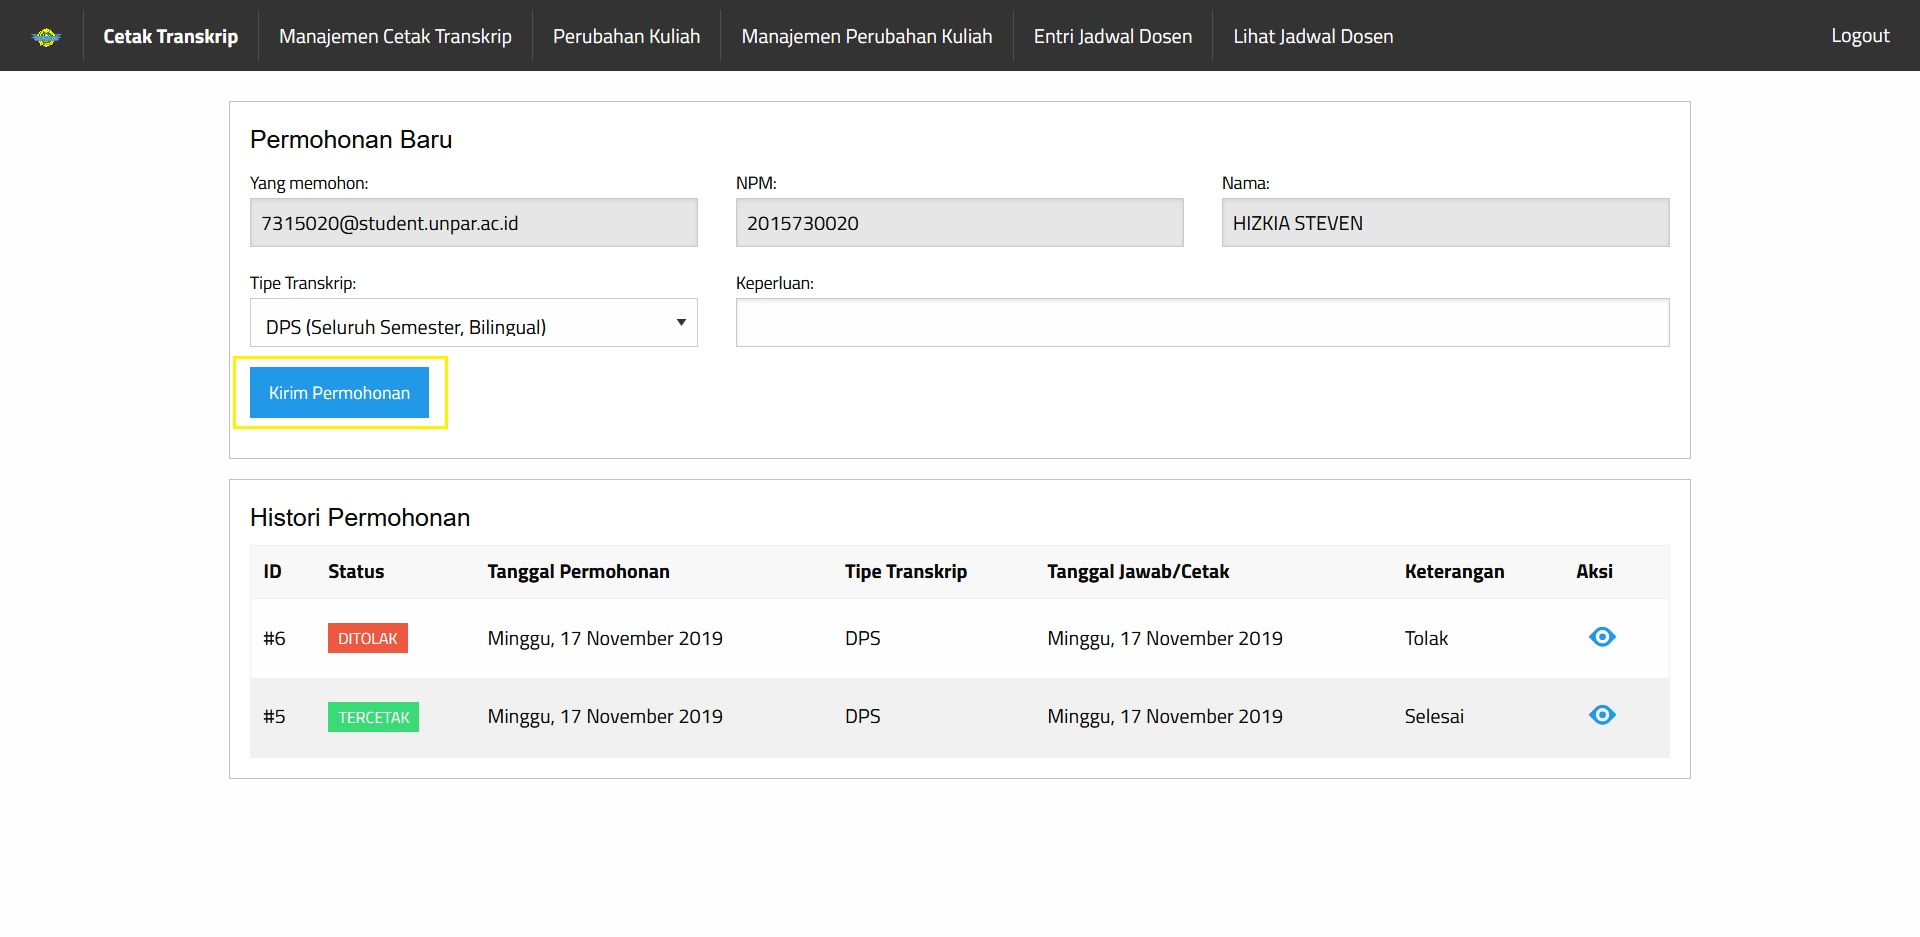
\includegraphics[scale=0.5]{kriteria-sukses-2-4-7-focus-visible}  
    \caption[Kriteria Sukses 2.4.7 - Indikator Fokus]{Kriteria Sukses 2.4.7 - Indikator Fokus}
    \label{fig:2.4.7_focus_visible}  
\end{figure}
Contoh tautan untuk halaman yang bermasalah: 

\url{https://bluetape.azurewebsites.net/TranskripRequest}.

\paragraph{Kriteria Sukses 2.4.8 \textit{Location}}
\label{par:kepatuhan_bluetape_kriteria_sukses_2.4.8}
(Sukses)\\

Kriteria ini sukses dipatuhi karena pada menu navigasi terdapat indikator yang menunjukkan halaman yang sedang dipilih oleh pengguna, indikator ini berupa penebalan ukuran tulisan.

\paragraph{Kriteria Sukses 2.4.9 \textit{Link Purpose (Link Only)}}
\label{par:kepatuhan_bluetape_kriteria_sukses_2.4.9}
(Tidak Sukses)\\

Kriteria ini tidak sukses dipatuhi karena pada halaman cetak transkrip, manajemen cetak transkrip, perubahan kuliah, dan manajemen perubahan kuliah terdapat tautan yang berisi konten bukan teks dan tidak terdapat teks yang dapat menjelaskan tujuan tautan tersebut. Kesalahan dapat dilihat pada potongan kode \ref{lst:2.4.9_tautan_tanpa_keterangan}. Tampilan pada halaman web dapat dilihat pada gambar \ref{fig:2.4.9_link_purpose_link_only}.

\begin{lstlisting}[frame=single, label={lst:2.4.9_tautan_tanpa_keterangan}, language=HTML, caption=Kriteria Sukses 2.4.9 - Tautan Tanpa Keterangan]
        </div>
        <a data-open="detail6">
            <i class="fi-eye"></i>
        </a>
    </td>
\end{lstlisting}

\begin{figure}[H]
	\centering  
	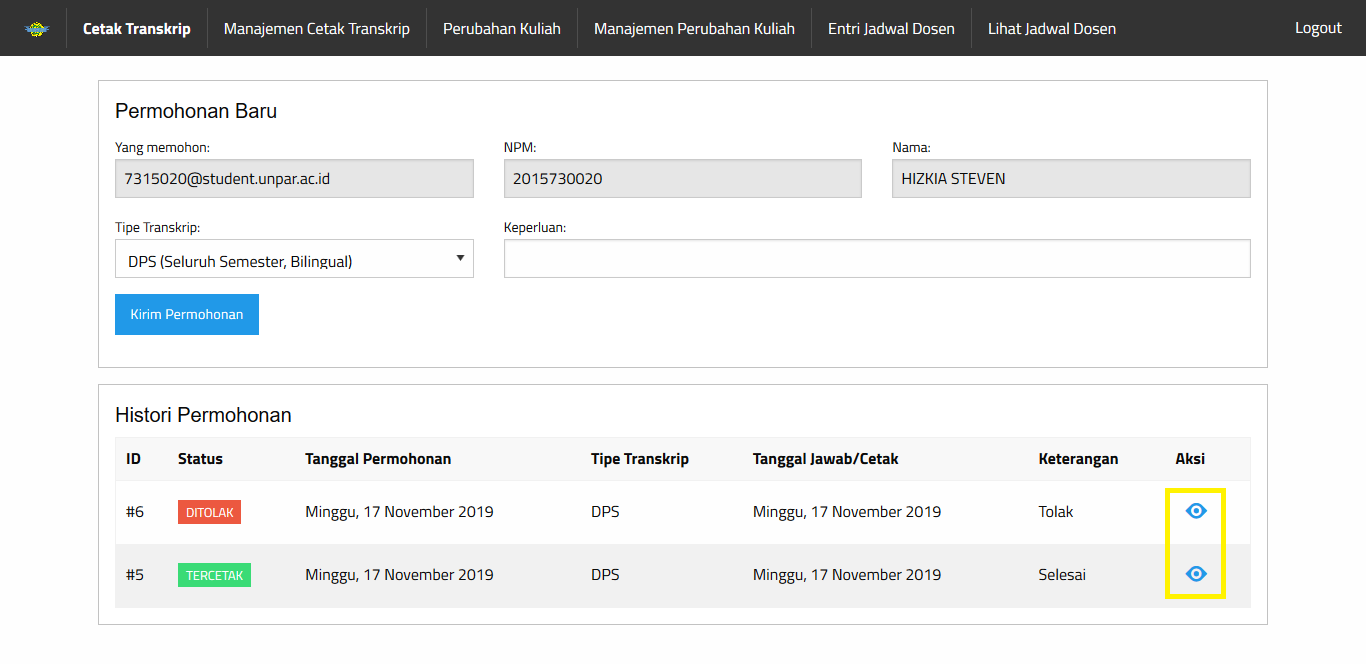
\includegraphics[scale=0.5]{kriteria-sukses-2-4-9-link-purpose-link-only}  
    \caption[Kriteria Sukses 2.4.9 - Tautan Tanpa Keterangan]{Kriteria Sukses 2.4.9 - Tautan Tanpa Keterangan}
    \label{fig:2.4.9_link_purpose_link_only}  
\end{figure} 
Contoh tautan untuk halaman yang bermasalah: 

\url{https://bluetape.azurewebsites.net/TranskripRequest}.

\paragraph{Kriteria Sukses 2.4.10 \textit{Section Headings}}
\label{par:kepatuhan_bluetape_kriteria_sukses_2.4.10}
(Tidak Sukses)\\

Kriteria ini tidak sukses dipatuhi karena terdapat penggunaan \textit{tag heading} yang tidak tepat secara struktur pada halaman cetak transkrip, manajemen cetak transkrip, perubahan kuliah, manajemen perubahan kuliah, dan entri jadwal dosen. Contoh kesalahan dapat dilihat pada potongan kode \ref{lst:1.3.1_heading_tidak_tepat} yang menampilkan kesalahan penggunaan \textit{tag heading} pada halaman cetak transkrip.

\begin{lstlisting}[frame=single, label={lst:2.4.10_heading_tidak_tepat}, language=HTML, caption=Kriteria Sukses 2.4.10 - Penggunaan \textit{Heading} Tidak Tepat]
    <div class="callout">
        <h5>Permohonan Baru</h5>
        <form method="POST" action="/TranskripRequest/add">
\end{lstlisting}
Contoh tautan untuk halaman yang bermasalah: 

\url{https://bluetape.azurewebsites.net/TranskripRequest}.

\subsubsection{\textit{Input Modalities}}
\label{subsubsec:kepatuhan_bluetape_input_modalities}

\paragraph{Kriteria Sukses 2.5.1 \textit{Pointer Gestures}}
\label{par:kepatuhan_bluetape_kriteria_sukses_2.5.1}
(Sukses)\\

Kriteria ini sukses dipatuhi karena pada halaman web BlueTape tidak terdapat fungsionalitas yang harus dijalankan dengan menggunakan \textit{multipoint} atau gestur berbasis \textit{path}.

\paragraph{Kriteria Sukses 2.5.2 \textit{Pointer Cancellation}}
\label{par:kepatuhan_bluetape_kriteria_sukses_2.5.2}
(Sukses)\\

Kriteria ini sukses dipatuhi karena setiap fungsionalitas yang dapat dioperasikan dengan kursor tunggal tidak memiliki \textit{down-event}.

\paragraph{Kriteria Sukses 2.5.3 \textit{Label in Name}}
\label{par:kepatuhan_bluetape_kriteria_sukses_2.5.3}
(Tidak Sukses)\\

Kriteria ini tidak sukses dipatuhi karena setiap komponen masukan yang memiliki label yang menyertakan teks, nama komponen tersebut tidak mengandung teks yang disajikan secara visual. Contoh kesalahan dapat dilihat pada potongan kode \ref{lst:2.5.3_teks_label_pada_nama}.

\begin{lstlisting}[frame=single, label={lst:2.5.3_teks_label_pada_nama}, language=HTML, caption=Kriteria Sukses 2.5.3 - Teks Label pada Atribut Nama]
    <div class="large-4 column">
        <label>Yang memohon:
            <input type="email" name="requestByEmail" 
            value="7315020@student.unpar.ac.id" readonly="readonly"/>
        </label>
    </div>
\end{lstlisting}
Contoh tautan untuk halaman yang bermasalah: 

\url{https://bluetape.azurewebsites.net/TranskripRequest}.

\paragraph{Kriteria Sukses 2.5.4 \textit{Motion Actuation}}
\label{par:kepatuhan_bluetape_kriteria_sukses_2.5.4}
(Sukses)\\

Kriteria ini sukses dipatuhi karena tidak terdapat fungsionalitas yang dapat dioperasikan oleh gerakan perangkat atau gerakan pengguna.

\paragraph{Kriteria Sukses 2.5.5 \textit{Target Size}}
\label{par:kepatuhan_bluetape_kriteria_sukses_2.5.5}
(Tidak Sukses)\\

Kriteria ini tidak sukses dipatuhi karena terdapat banyak elemen yang dapat menerima masukan kursor dan ukurannya diatur oleh penulis namun memiliki ukuran kurang dari 44 kali 44 piksel \textit{CSS}. Contoh tampilan pada halaman web dapat dilihat pada gambar \ref{fig:2.5.5_target_size}. 

\begin{figure}[H]
	\centering  
	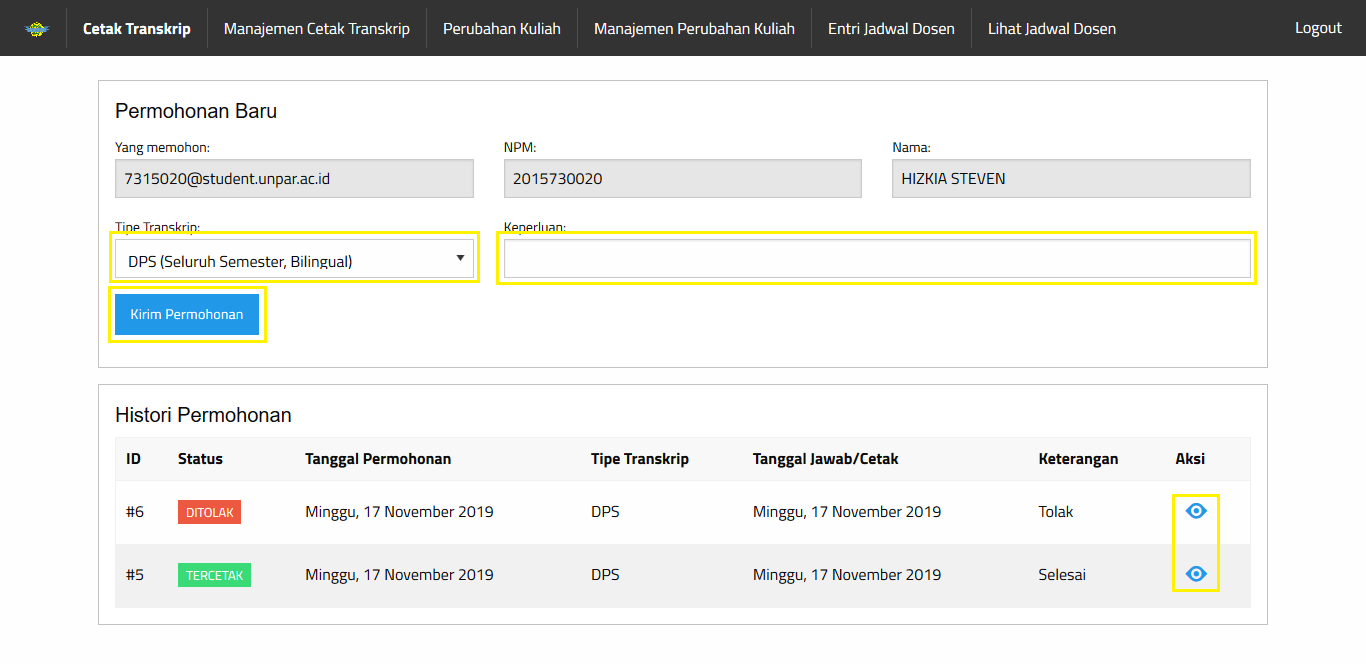
\includegraphics[scale=0.5]{kriteria-sukses-2-5-5-target-size}  
    \caption[Kriteria Sukses 2.5.5 - Ukuran Elemen]{Kriteria Sukses 2.5.5 - Ukuran Elemen}
    \label{fig:2.5.5_target_size}  
\end{figure} 
Contoh tautan untuk halaman yang bermasalah: 

\url{https://bluetape.azurewebsites.net/TranskripRequest}.

\paragraph{Kriteria Sukses 2.5.6 \textit{Concurrent Input Mechanisms}}
\label{par:kepatuhan_bluetape_kriteria_sukses_2.5.6}
(Sukses)\\

Kriteria ini sukses dipatuhi karena konten web BlueTape tidak membatasi penggunaan modalitas masukan yang tersedia pada platform.

\subsection{\textit{Understandable}}
\label{subsec:kepatuhan_bluetape_understandable}

\subsubsection{\textit{Readable}}
\label{subsubsec:kepatuhan_bluetape_readable}

\paragraph{Kriteria Sukses 3.1.1 \textit{Language of Page}}
\label{par:kepatuhan_bluetape_kriteria_sukses_3.1.1}
(Tidak Sukses)\\

Kriteria ini tidak sukses dipatuhi karena bahasa manusia \textit{default} yang digunakan pada halaman web BlueTape tidak sesuai dengan konten yang disajikan pada halaman tersebut. Bahasa manusia \textit{default} yang digunakan pada halaman web BlueTape adalah bahasa Inggris sementara konten disajikan dalam bahasa Indonesia. Contoh kesalahan dapat dilihat pada potongan kode \ref{lst:3.1.1_bahasa_halaman}.

\begin{lstlisting}[frame=single, label={lst:3.1.1_bahasa_halaman}, language=HTML, caption=Kriteria Sukses 3.1.1 - Bahasa yang Tidak Sesuai]
    // Setelan bahasa diatur menjadi bahasa Inggris
    <!DOCTYPE html>
        <html class="no-js" lang="en">
    <head>

    // Konten disajikan dalam bahasa Indonesia
    <div class="large-4 column">
        <label>Yang memohon:
            <input type="email" name="requestByEmail" 
            value="7315020@student.unpar.ac.id" readonly="readonly"/>
        </label>
    </div>
    <div class="large-4 column">
        <label>NPM:
            <input type="text" value="2015730020" 
            readonly="readonly"/>
        </label>
    </div>
    <div class="large-4 column">
        <label>Nama:
            <input type="text" name="requestByName" 
            value="HIZKIA STEVEN" readonly="readonly"/>
        </label>
    </div>
\end{lstlisting}
Contoh tautan untuk halaman yang bermasalah: 

\url{https://bluetape.azurewebsites.net/TranskripRequest}.

\paragraph{Kriteria Sukses 3.1.2 \textit{Language of Parts}}
\label{par:kepatuhan_bluetape_kriteria_sukses_3.1.2}
(Tidak Sukses)\\

Kriteria ini tidak sukses dipatuhi karena pada halaman web BlueTape terdapat konten teks dalam bahasa Inggris namun konten tersebut tidak memiliki atribut \textit{lang}. Konten yang dimaksud adalah:

\begin{itemize}
    \item Pada bagian navigasi menu terdapat elemen dengan teks "Logout". Letak kesalahan dapat dilihat pada potongan kode \ref{lst:3.1.2_bahasa_pada_navigasi}. Contoh tampilan pada halaman web dapat dilihat pada gambar \ref{fig:3.1.2_language_of_parts_1}. 
    \begin{lstlisting}[frame=single, label={lst:3.1.2_bahasa_pada_navigasi}, language=HTML, caption=Kriteria Sukses 3.1.2 - Bahasa yang Tidak Sesuai pada Menu Navigasi]
        <ul class="menu">
            <li><a href="/auth/logout">Logout</a></li>
        </ul>
    \end{lstlisting}
    
    \begin{figure}[H]
        \centering  
        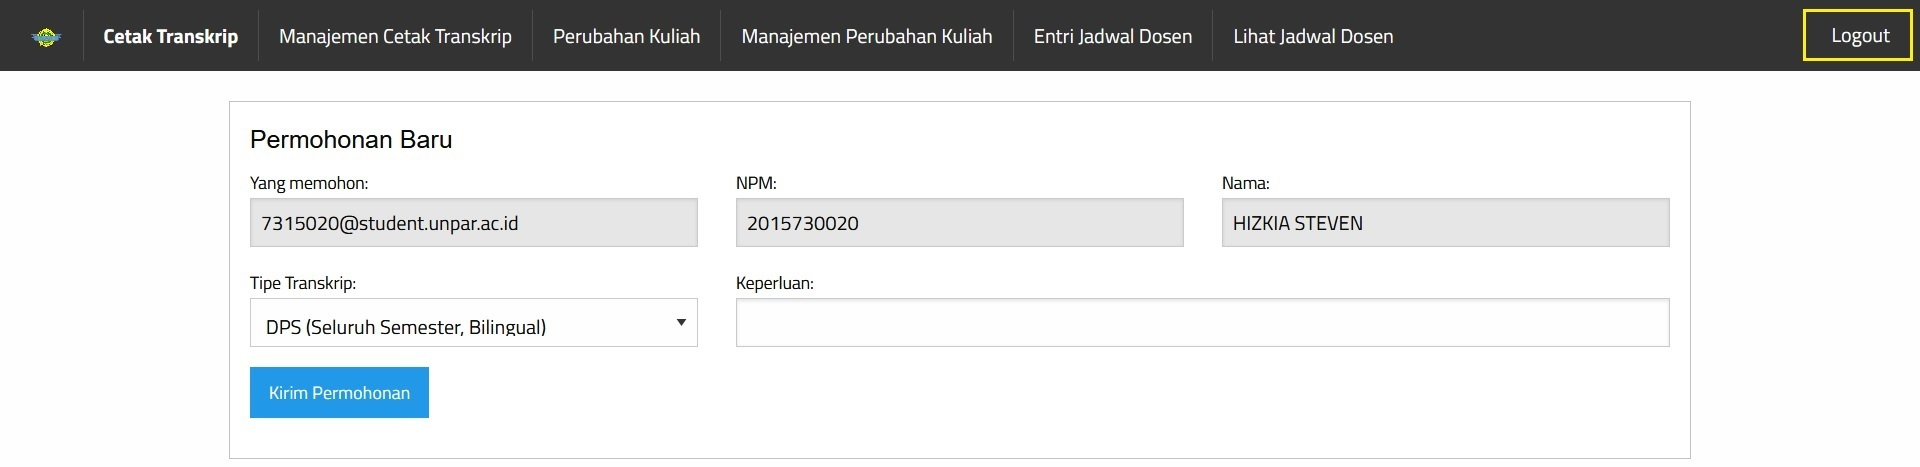
\includegraphics[scale=0.5]{kriteria-sukses-3-1-2-language-of-parts-1}  
        \caption[Kriteria Sukses 3.1.2 - Bahasa pada Menu Navigasi]{Kriteria Sukses 3.1.2 - Bahasa pada Menu Navigasi}
        \label{fig:3.1.2_language_of_parts_1}  
    \end{figure}

    \item Pada halaman entri jadwal dosen terdapat tombol dengan teks "Delete All". Letak kesalahan dapat dilihat pada potongan kode \ref{lst:3.1.2_bahasa_pada_halaman_entri_jadwal_dosen_1}. Contoh tampilan pada halaman web dapat dilihat pada gambar \ref{fig:3.1.2_language_of_parts_2}. 
    \begin{lstlisting}[frame=single, label={lst:3.1.2_bahasa_pada_halaman_entri_jadwal_dosen_1}, language=HTML, caption=Kriteria Sukses 3.1.2 - Bahasa yang Tidak Sesuai pada Halaman Entri Jadwal Dosen 1]
        ?>
        <a href="/EntriJadwalDosen/deleteAll/export/" 
        class="alert button" onClick="return konfirmasi();">
        Delete All</a>
        <a href="/EntriJadwalDosen/export/" 
        class="button">Ekspor ke XLS</a>
    \end{lstlisting}
    
    \begin{figure}[H]
        \centering  
        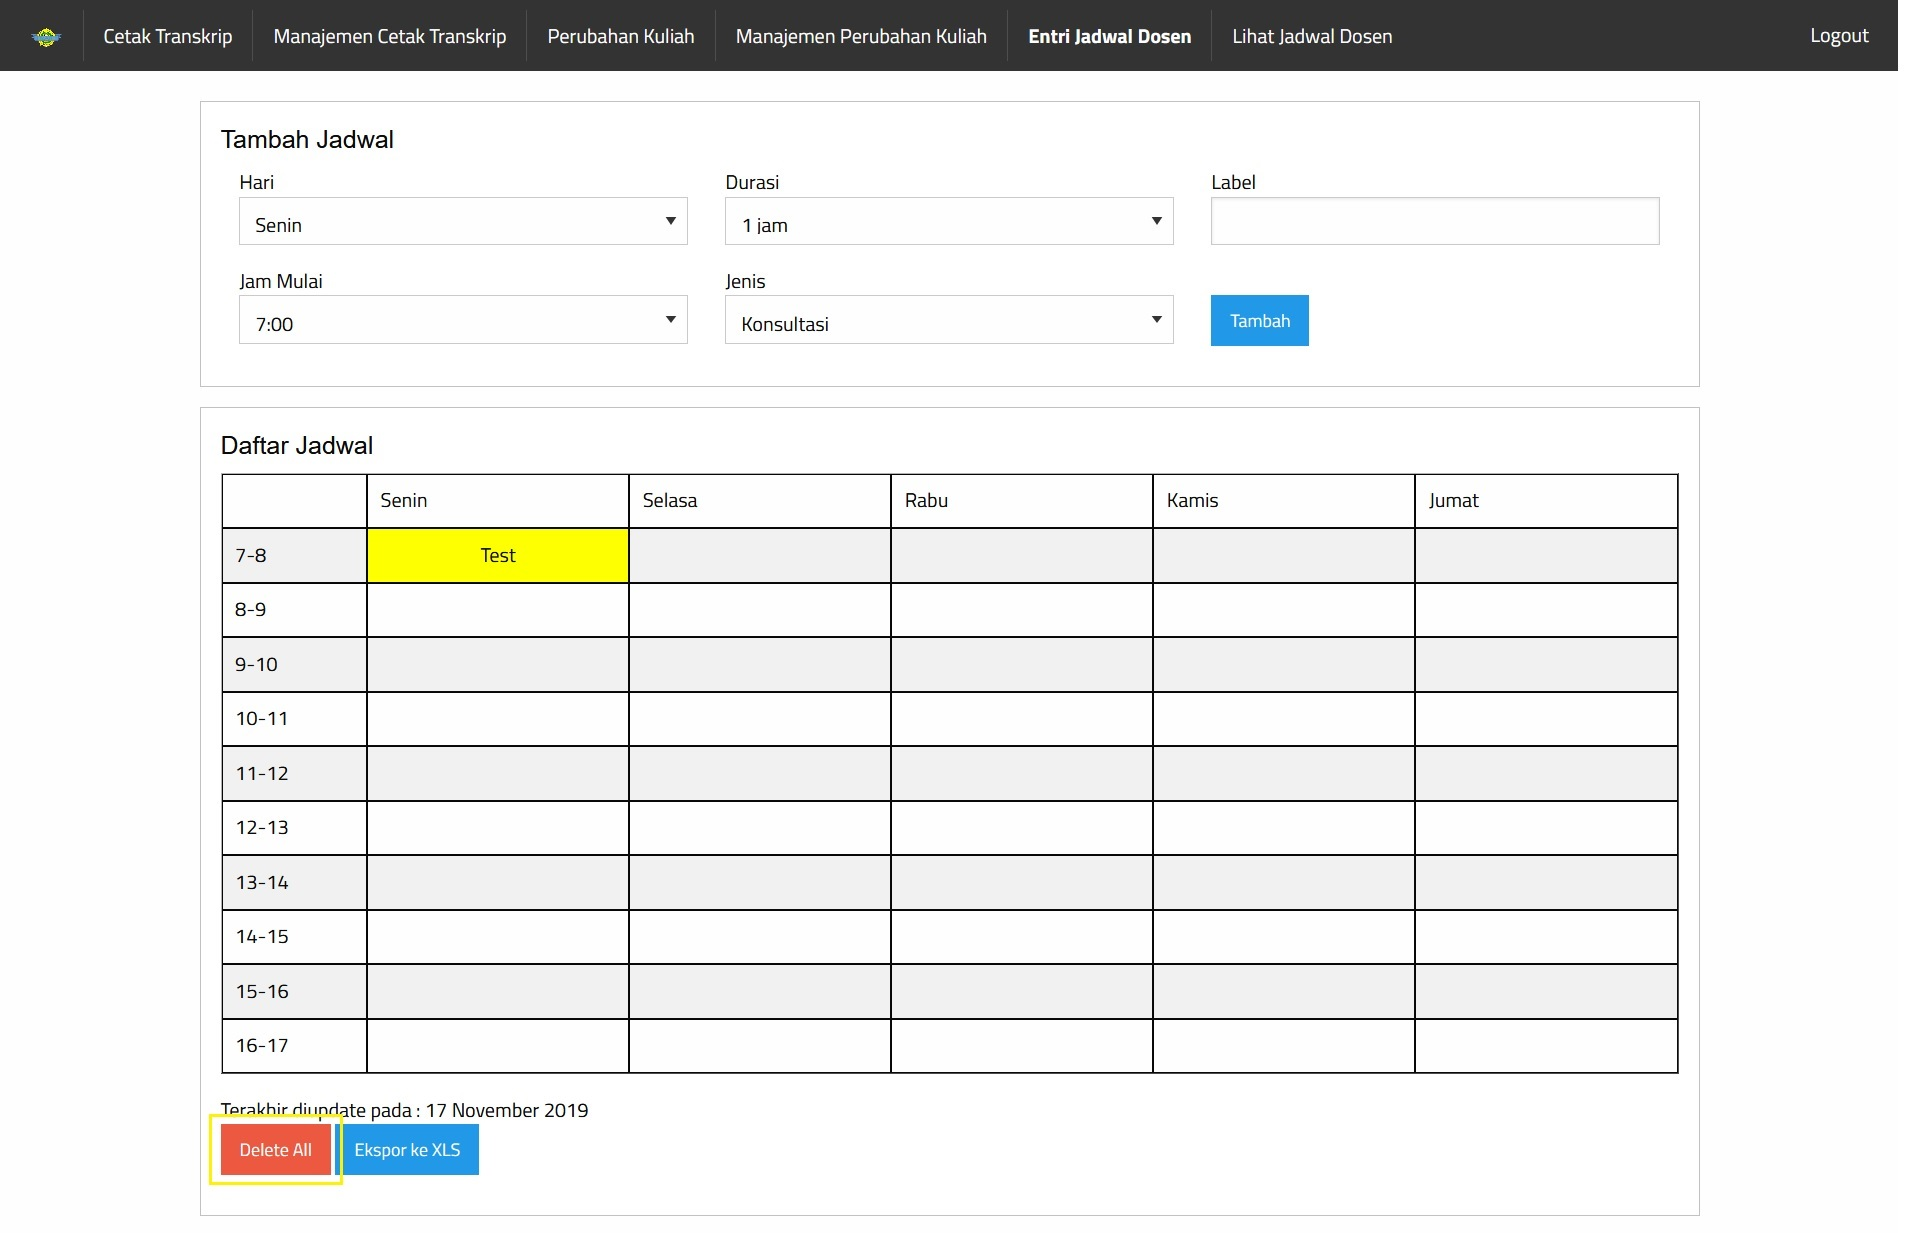
\includegraphics[scale=0.5]{kriteria-sukses-3-1-2-language-of-parts-2}  
        \caption[Kriteria Sukses 3.1.2 - Bahasa pada Halaman Entri Jadwal Dosen 1]{Kriteria Sukses 3.1.2 - Bahasa pada Halaman Entri Jadwal Dosen 1}
        \label{fig:3.1.2_language_of_parts_2}  
    \end{figure}
    Tautan untuk halaman yang bermasalah: 
    
    \url{https://bluetape.azurewebsites.net/EntriJadwalDosen}.

    \item Pada halaman entri jadwal dosen bagian "Edit Jadwal" terdapat tombol dengan teks "Save" dan tombol dengan teks "Delete". Letak kesalahan dapat dilihat pada potongan kode \ref{lst:3.1.2_bahasa_pada_halaman_entri_jadwal_dosen_2}. Contoh tampilan pada halaman web dapat dilihat pada gambar \ref{fig:3.1.2_language_of_parts_3}. 
    \begin{lstlisting}[frame=single, label={lst:3.1.2_bahasa_pada_halaman_entri_jadwal_dosen_2}, language=HTML, caption=Kriteria Sukses 3.1.2 - Bahasa yang Tidak Sesuai pada Halaman Entri Jadwal Dosen 2]
        // Tombol "Save"
        <div class="large-2 column">
            <input type="submit" 
            name="submitId8" class="button" 
            value="Save">
            </form>
        </div>

        // Tombol "Delete"
        <form name="formDelete8" method="POST"
        action="/EntriJadwalDosen/delete/8">    
            <input type="hidden" name="csrf_token" 
            value="3c159eae7bc953dd591b679c080ed066" />
            <input id="deletebtn8" name="8" type="submit"
            class="alert button" value="Delete">
        </form><div>
    \end{lstlisting}
    
    \begin{figure}[H]
        \centering  
        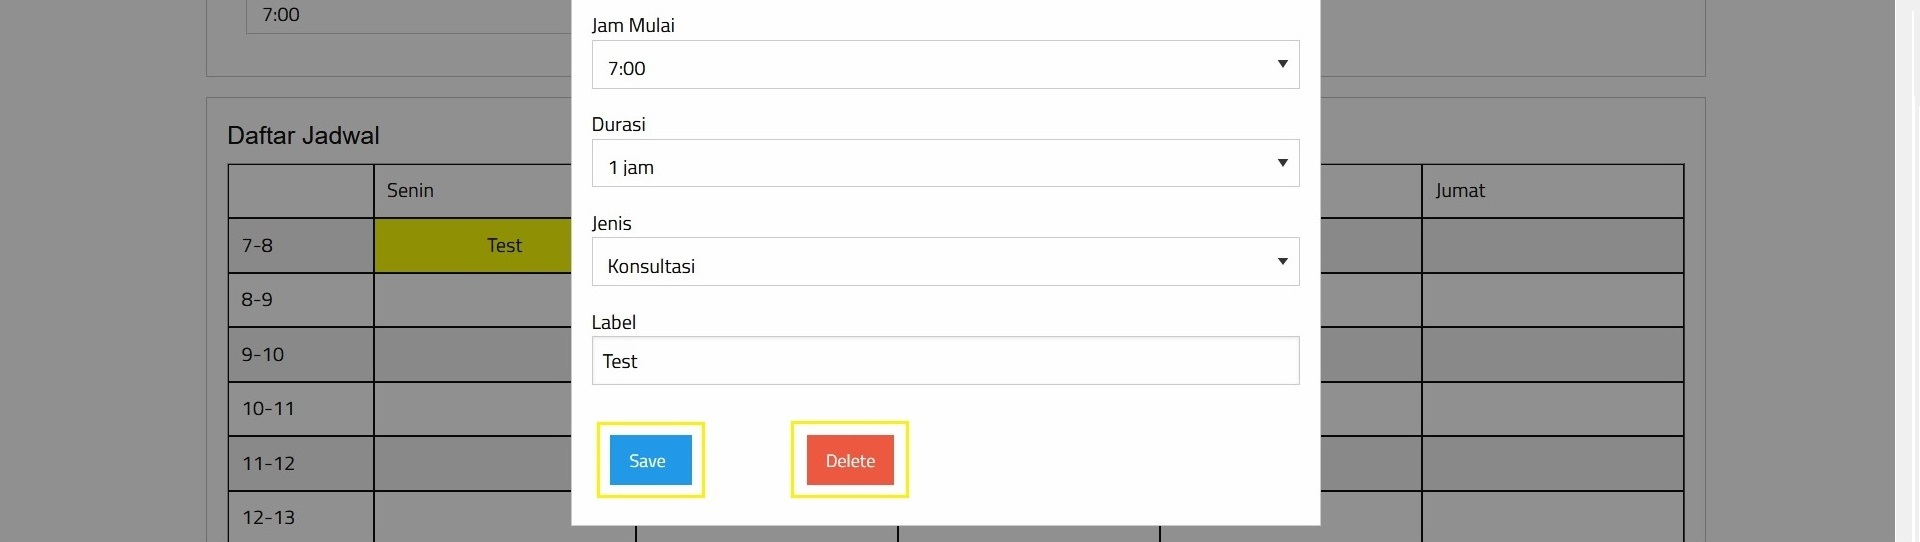
\includegraphics[scale=0.5]{kriteria-sukses-3-1-2-language-of-parts-3}  
        \caption[Kriteria Sukses 3.1.2 - Bahasa pada Halaman Entri Jadwal Dosen 2]{Kriteria Sukses 3.1.2 - Bahasa pada Halaman Entri Jadwal Dosen 2}
        \label{fig:3.1.2_language_of_parts_3}  
    \end{figure}
    Tautan untuk halaman yang bermasalah: 
    
    \url{https://bluetape.azurewebsites.net/EntriJadwalDosen}.

\end{itemize}

\paragraph{Kriteria Sukses 3.1.3 \textit{Unusual Words}}
\label{par:kepatuhan_bluetape_kriteria_sukses_3.1.3}
(Tidak Sukses)\\

Kriteria ini tidak sukses dipatuhi karena terdapat kata-kata yang digunakan dengan cara yang tidak lazim atau terbatas namun tidak tersedia mekanisme untuk mengidentifikasi definisi spesifik dari kata-kata tersebut. Kata-kata yang dimaksud adalah:

\begin{itemize}
    \item Pada halaman perubahan kuliah, tombol dengan teks "Tambah Pertemuan Ekstra". Letak kesalahan dapat dilihat pada potongan kode \ref{lst:3.1.3_kata_pada_halaman_perubahan_kuliah}. Contoh tampilan pada halaman web dapat dilihat pada gambar \ref{fig:3.1.3_unusual_words_1}.
    \begin{lstlisting}[frame=single, label={lst:3.1.3_kata_pada_halaman_perubahan_kuliah}, language=HTML, caption=Kriteria Sukses 3.1.3 - Kata yang Tak Lazim pada Halaman Perubahan Kuliah]
        <div class="large-12 column">
            <input type="submit" class="button" 
            value="Kirim Permohonan">
            <a href="#" id="addToButton" 
            class="button secondary">Tambah Pertemuan Ekstra</a>
        </div>
    \end{lstlisting}
    
    \begin{figure}[H]
        \centering  
        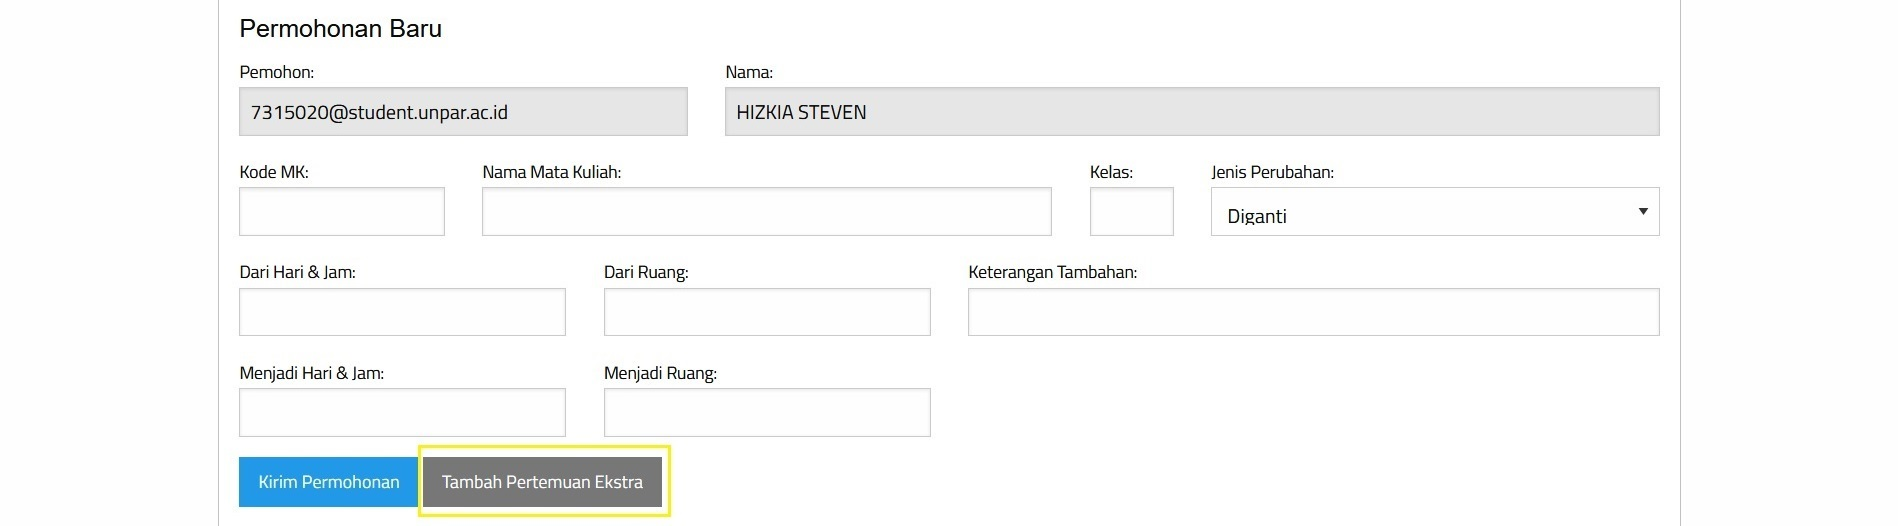
\includegraphics[scale=0.5]{kriteria-sukses-3-1-3-unusual-words-1}  
        \caption[Kriteria Sukses 3.1.3 - Kata yang Tak Lazim pada Halaman Perubahan Kuliah]{Kriteria Sukses 3.1.3 - Kata yang Tak Lazim pada Halaman Perubahan Kuliah}
        \label{fig:3.1.3_unusual_words_1}  
    \end{figure}
    Tautan untuk halaman yang bermasalah: 
    
    \url{https://bluetape.azurewebsites.net/PerubahanKuliahRequest}.

    \item Pada halaman entri jadwal dosen, tombol dengan teks "Ekspor ke XLS". Letak kesalahan dapat dilihat pada potongan kode \ref{lst:3.1.3_kata_pada_halaman_entri_jadwal_dosen}. Contoh tampilan pada halaman web dapat dilihat pada gambar \ref{fig:3.1.3_unusual_words_2}.
    \begin{lstlisting}[frame=single, label={lst:3.1.3_kata_pada_halaman_entri_jadwal_dosen}, language=HTML, caption=Kriteria Sukses 3.1.3 - Kata yang Tak Lazim pada Halaman Entri Jadwal Dosen]
        <a href="/EntriJadwalDosen/export/" class="button">
            Ekspor ke XLS
        </a>
    \end{lstlisting}
    
    \begin{figure}[H]
        \centering  
        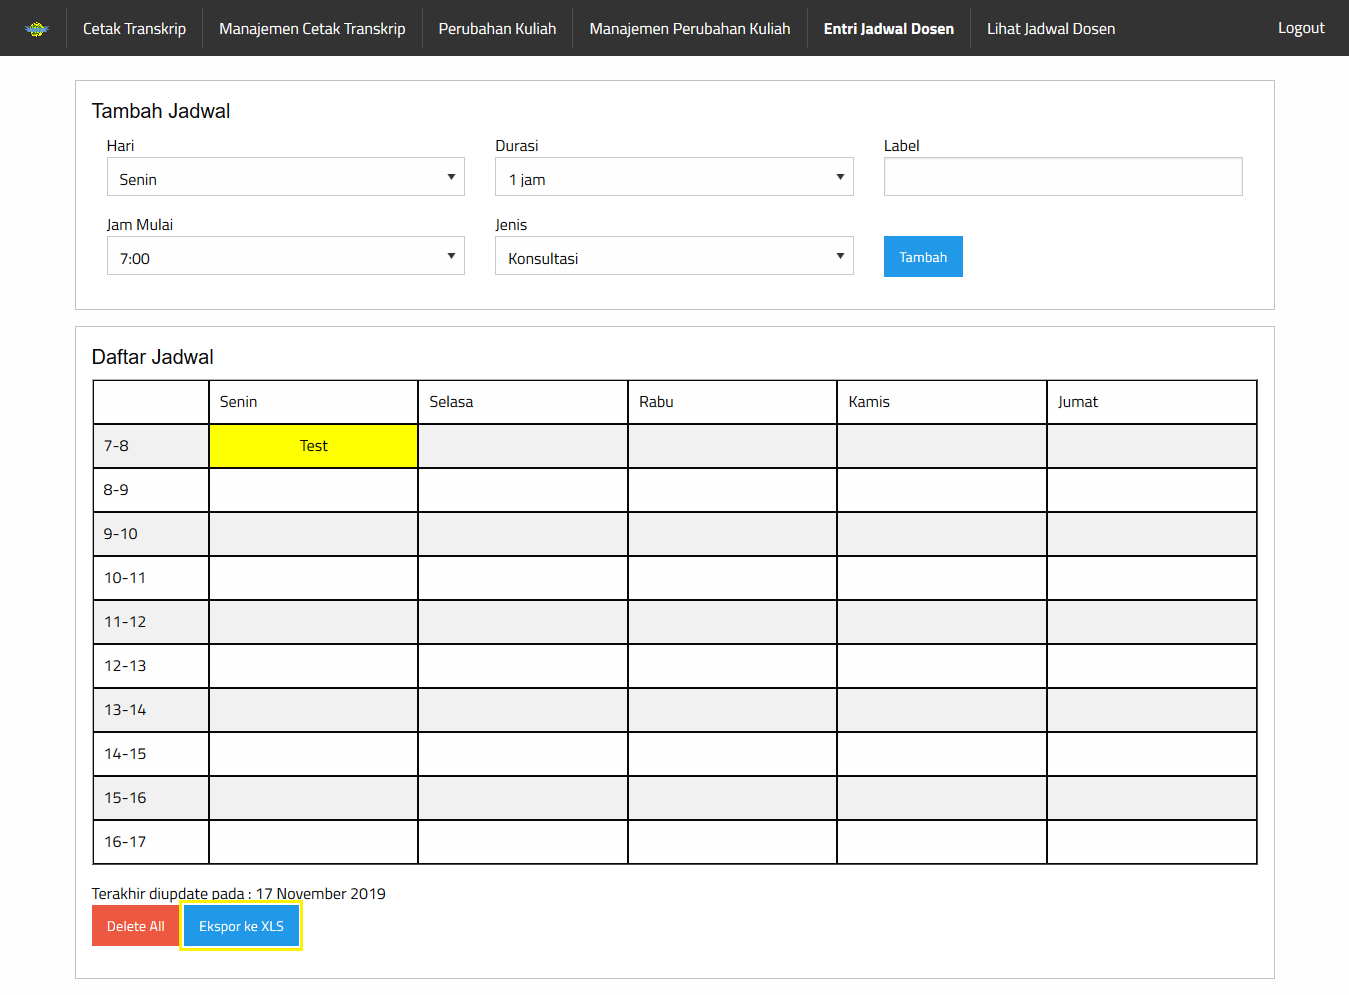
\includegraphics[scale=0.5]{kriteria-sukses-3-1-3-unusual-words-2}  
        \caption[Kriteria Sukses 3.1.3 - Kata yang Tak Lazim pada Halaman Entri Jadwal Dosen]{Kriteria Sukses 3.1.3 - Kata yang Tak Lazim pada Halaman Entri Jadwal Dosen}
        \label{fig:3.1.3_unusual_words_2}  
    \end{figure}
    Tautan untuk halaman yang bermasalah: 
    
    \url{https://bluetape.azurewebsites.net/EntriJadwalDosen}.

    \item Pada halaman lihat jadwal dosen, tombol dengan teks "Ekspor ke XLS". Letak kesalahan dapat dilihat pada potongan kode \ref{lst:3.1.3_kata_pada_halaman_lihat_jadwal_dosen}. Contoh tampilan pada halaman web dapat dilihat pada gambar \ref{fig:3.1.3_unusual_words_3}.
    \begin{lstlisting}[frame=single, label={lst:3.1.3_kata_pada_halaman_lihat_jadwal_dosen}, language=HTML, caption=Kriteria Sukses 3.1.3 - Kata yang Tak Lazim pada Halaman Lihat Jadwal Dosen]
            <?php
            }
            ?>
        <a href="/LihatJadwalDosen/export/" 
        class="button">Ekspor ke XLS</a>
        </div> 
    \end{lstlisting}
    
    \begin{figure}[H]
        \centering  
        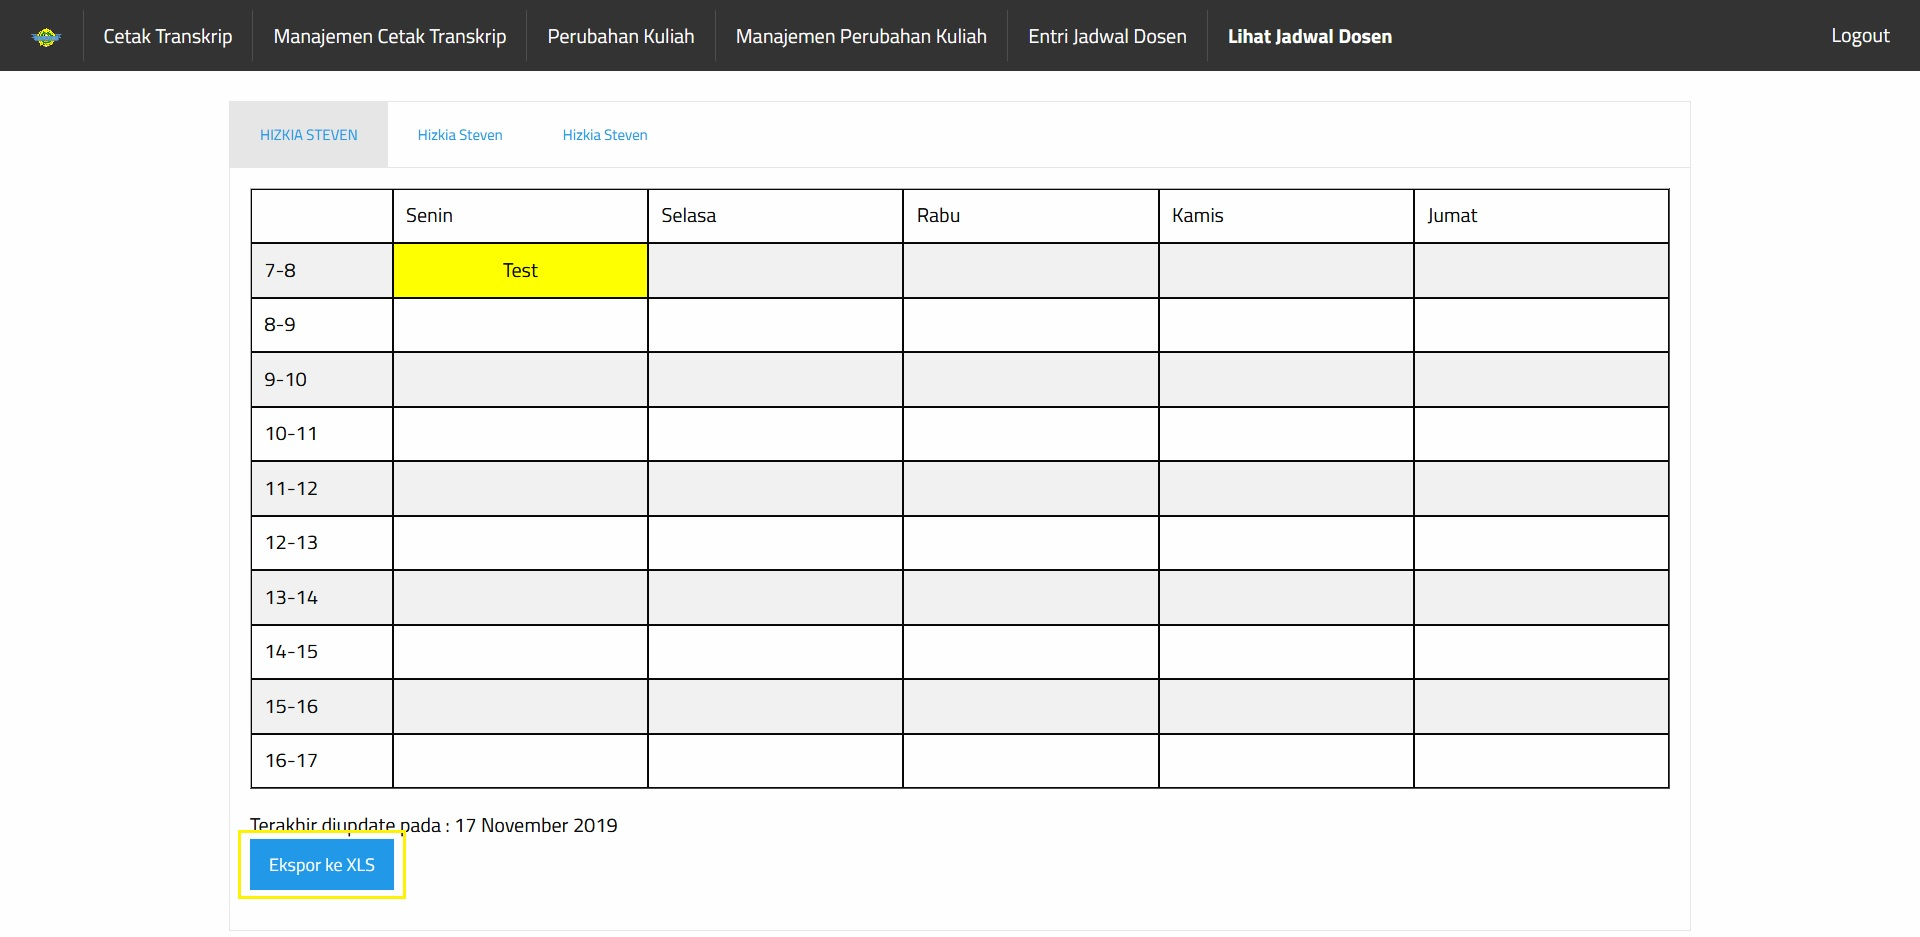
\includegraphics[scale=0.5]{kriteria-sukses-3-1-3-unusual-words-3}  
        \caption[Kriteria Sukses 3.1.3 - Kata yang Tak Lazim pada Halaman Lihat Jadwal Dosen]{Kriteria Sukses 3.1.3 - Kata yang Tak Lazim pada Halaman Lihat Jadwal Dosen}
        \label{fig:3.1.3_unusual_words_3}  
    \end{figure}
    Tautan untuk halaman yang bermasalah: 
    
    \url{https://bluetape.azurewebsites.net/LihatJadwalDosen}.

\end{itemize}

\paragraph{Kriteria Sukses 3.1.4 \textit{Abbreviations}}
\label{par:kepatuhan_bluetape_kriteria_sukses_3.1.4}
(Tidak Sukses)\\

Kriteria ini tidak sukses dipatuhi karena tidak tersedia mekanisme untuk mengidentifikasi kepanjangan dari singkatan. Singkatan-singkatan yang terdapat pada halaman web BlueTape, antara lain:

\begin{itemize}
    \item Pada halaman cetak transkrip terdapat singkatan "NPM" dan "DPS". Letak kesalahan dapat dilihat pada potongan kode \ref{lst:3.1.4_singkatan_pada_halaman_cetak_transkrip}. Contoh tampilan pada halaman web dapat dilihat pada gambar \ref{fig:3.1.4_abbreviations_1}.
    \begin{lstlisting}[frame=single, label={lst:3.1.4_singkatan_pada_halaman_cetak_transkrip}, language=HTML, caption=Kriteria Sukses 3.1.4 - Singkatan pada Halaman Cetak Transkrip]
        // Singkatan "NPM"
        <div class="large-4 column">
            <label>NPM:
                <input type="text" value="2015730020" 
                readonly="readonly"/>
            </label>
        </div>
        
        // Singkatan "DPS"
        <select name="requestType">
            <option value="DPS">
                DPS (Seluruh Semester, Bilingual)
            </option>
        </select>
    \end{lstlisting}

    \begin{figure}[H]
        \centering  
        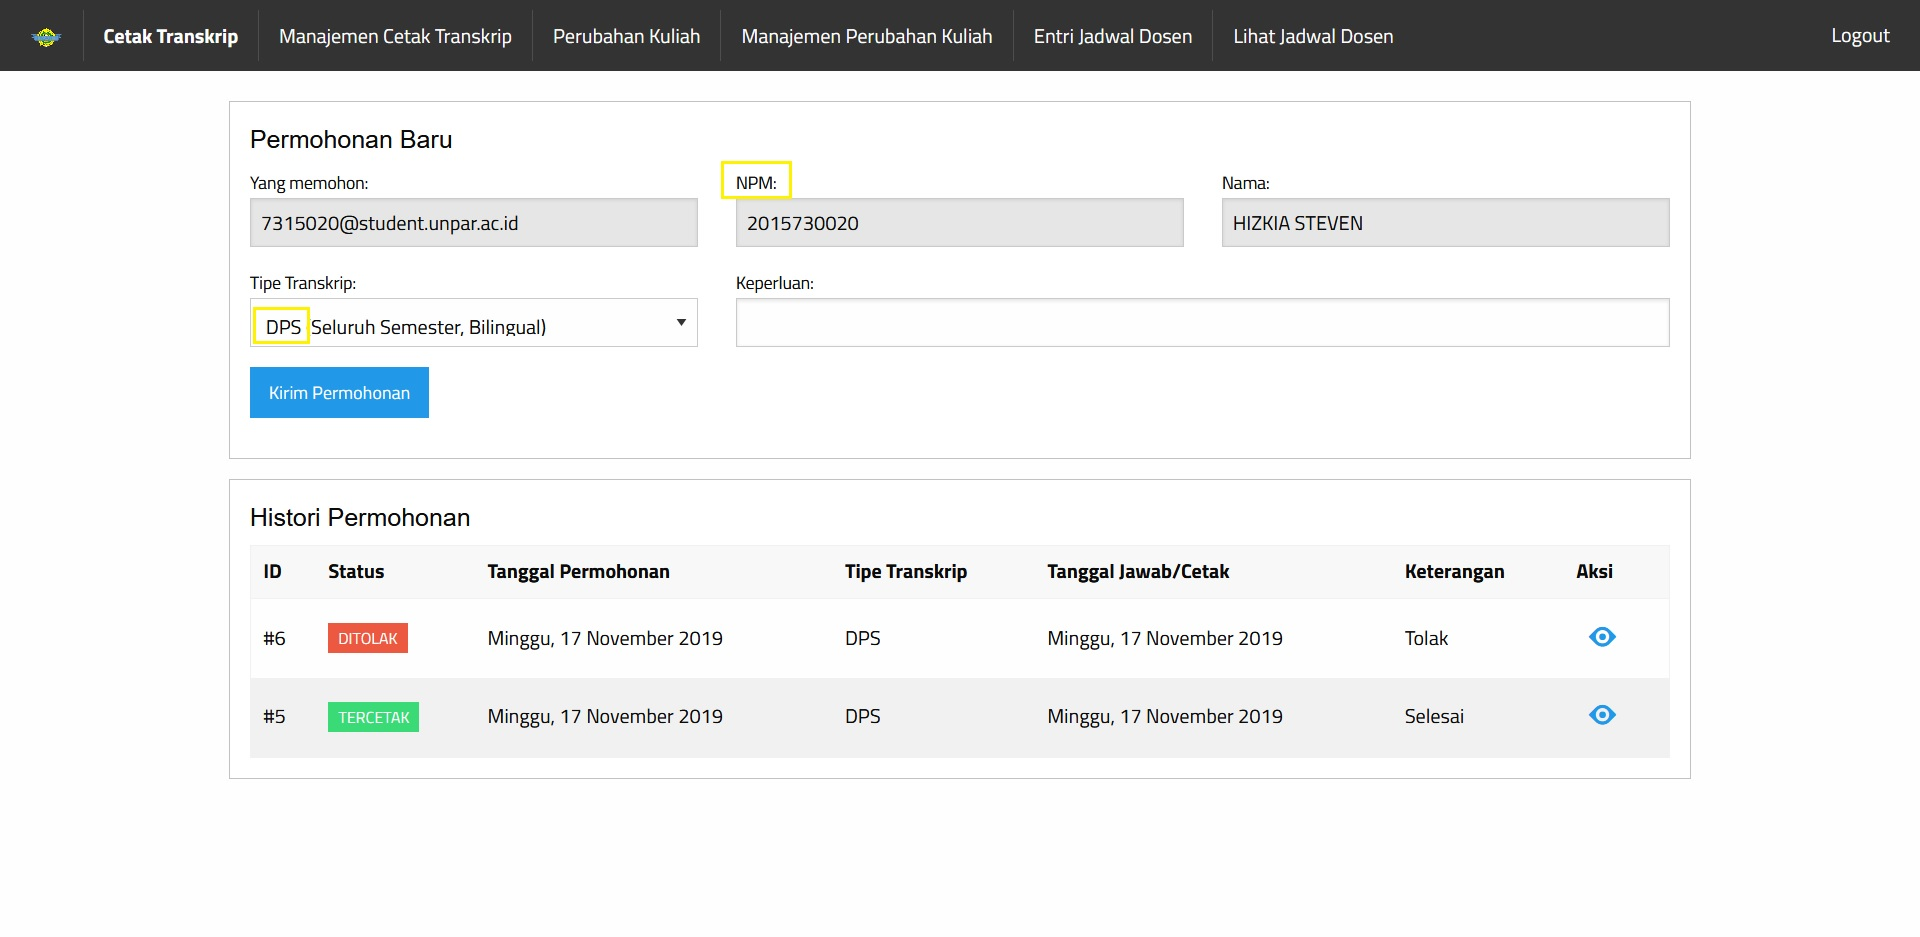
\includegraphics[scale=0.5]{kriteria-sukses-3-1-4-abbreviations-1}  
        \caption[Kriteria Sukses 3.1.4 - Singkatan pada Halaman Cetak Transkrip]{Kriteria Sukses 3.1.4 - Singkatan pada Halaman Cetak Transkrip}
        \label{fig:3.1.4_abbreviations_1}  
    \end{figure}
    Tautan untuk halaman yang bermasalah: 
    
    \url{https://bluetape.azurewebsites.net/TranskripRequest}.

    \item Pada halaman manajemen cetak transkrip terdapat singkatan "NPM". Letak kesalahan dapat dilihat pada potongan kode \ref{lst:3.1.4_singkatan_pada_halaman_manajemen_cetak_transkrip}. Contoh tampilan pada halaman web dapat dilihat pada gambar \ref{fig:3.1.4_abbreviations_2}.
    \begin{lstlisting}[frame=single, label={lst:3.1.4_singkatan_pada_halaman_manajemen_cetak_transkrip}, language=HTML, caption=Kriteria Sukses 3.1.4 - Singkatan pada Halaman Manajemen Cetak Transkrip]
        <div class="input-group">
            <span class="input-group-label">Cari NPM:</span>
            <input name="npm" class="input-group-field" 
            type="text" placeholder="2013730013" 
            maxlength="10" minlength="10"/>
    \end{lstlisting}

    \begin{figure}[H]
        \centering  
        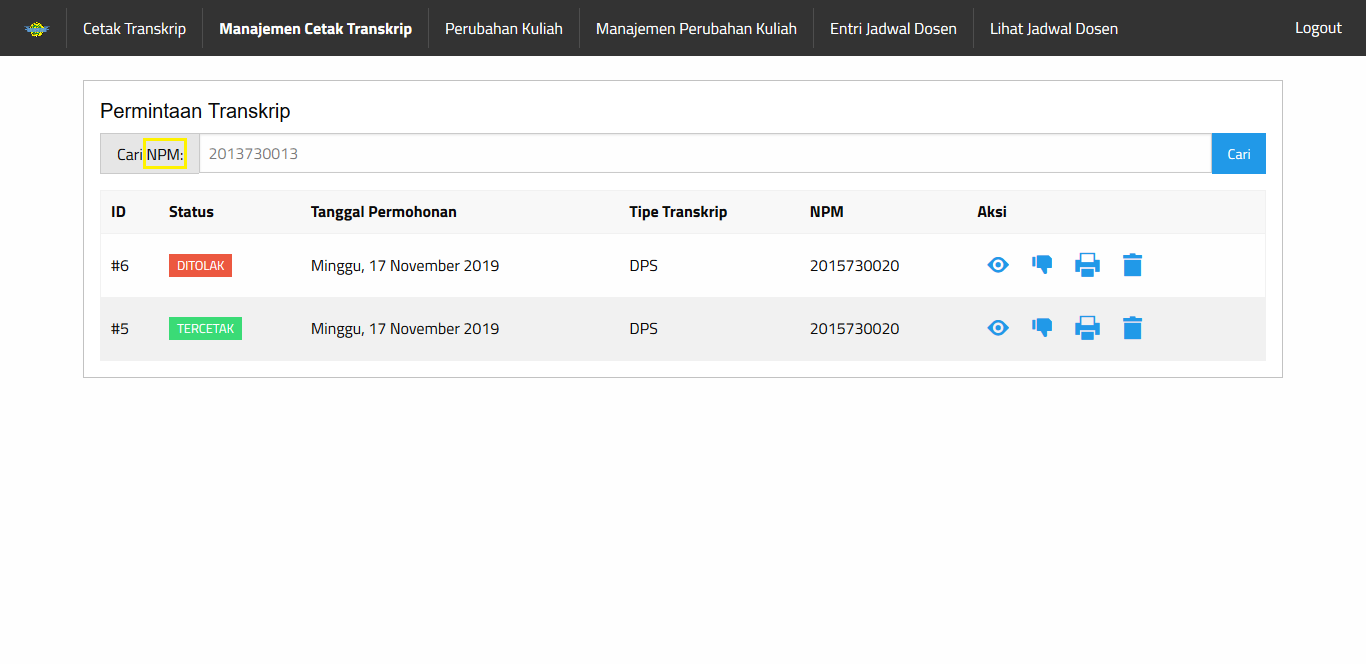
\includegraphics[scale=0.5]{kriteria-sukses-3-1-4-abbreviations-2}  
        \caption[Kriteria Sukses 3.1.4 - Singkatan pada Halaman Manajemen Cetak Transkrip]{Kriteria Sukses 3.1.4 - Singkatan pada Halaman Manajemen Cetak Transkrip}
        \label{fig:3.1.4_abbreviations_2}  
    \end{figure}
    Tautan untuk halaman yang bermasalah: 
    
    \url{https://bluetape.azurewebsites.net/TranskripManage}.

    \item Pada halaman perubahan kuliah terdapat singkatan "MK". Letak kesalahan dapat dilihat pada potongan kode \ref{lst:3.1.4_singkatan_pada_halaman_perubahan_kuliah}. Contoh tampilan pada halaman web dapat dilihat pada gambar \ref{fig:3.1.4_abbreviations_3}.
    \begin{lstlisting}[frame=single, label={lst:3.1.4_singkatan_pada_halaman_perubahan_kuliah}, language=HTML, caption=Kriteria Sukses 3.1.4 - Singkatan pada Halaman Perubahan Kuliah]
        <div class="large-2 column">
            <label>Kode MK:
                <input type="text" name="mataKuliahCode" required 
                maxlength="9" pattern="[A-Z]{3}[0-9]{3}([0-9]{3})?" 
                title="Kode MK dalam format XYZ123"/>
    \end{lstlisting}

    \begin{figure}[H]
        \centering  
        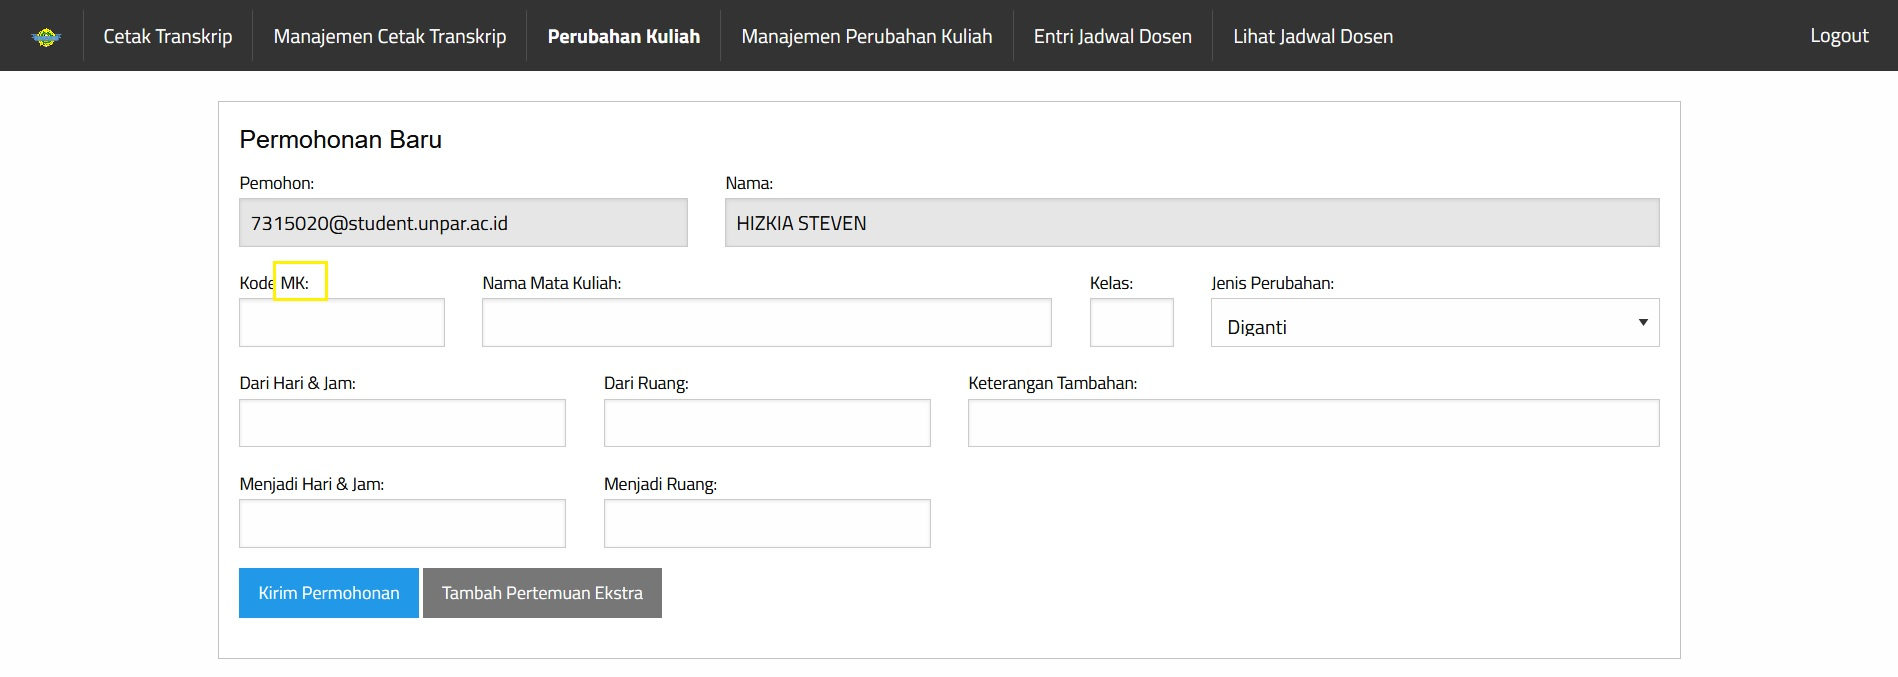
\includegraphics[scale=0.5]{kriteria-sukses-3-1-4-abbreviations-3}  
        \caption[Kriteria Sukses 3.1.4 - Singkatan pada Halaman Perubahan Kuliah]{Kriteria Sukses 3.1.4 - Singkatan pada Halaman Perubahan Kuliah}
        \label{fig:3.1.4_abbreviations_3}  
    \end{figure}
    Tautan untuk halaman yang bermasalah: 
    
    \url{https://bluetape.azurewebsites.net/PerubahanKuliahRequest}.

    \item Pada halaman manajemen perubahan kuliah terdapat singkatan "MK". Letak kesalahan dapat dilihat pada potongan kode \ref{lst:3.1.4_singkatan_pada_halaman_manajemen_perubahan_kuliah}. Contoh tampilan pada halaman web dapat dilihat pada gambar \ref{fig:3.1.4_abbreviations_4}.
    \begin{lstlisting}[frame=single, label={lst:3.1.4_singkatan_pada_halaman_manajemen_perubahan_kuliah}, language=HTML, caption=Kriteria Sukses 3.1.4 - Singkatan pada Halaman Manajemen Perubahan Kuliah]
        <th>Tanggal Permohonan</th>
        <th>Kode MK</th>
        <th>Perubahan</th>
    \end{lstlisting}

    \begin{figure}[H]
        \centering  
        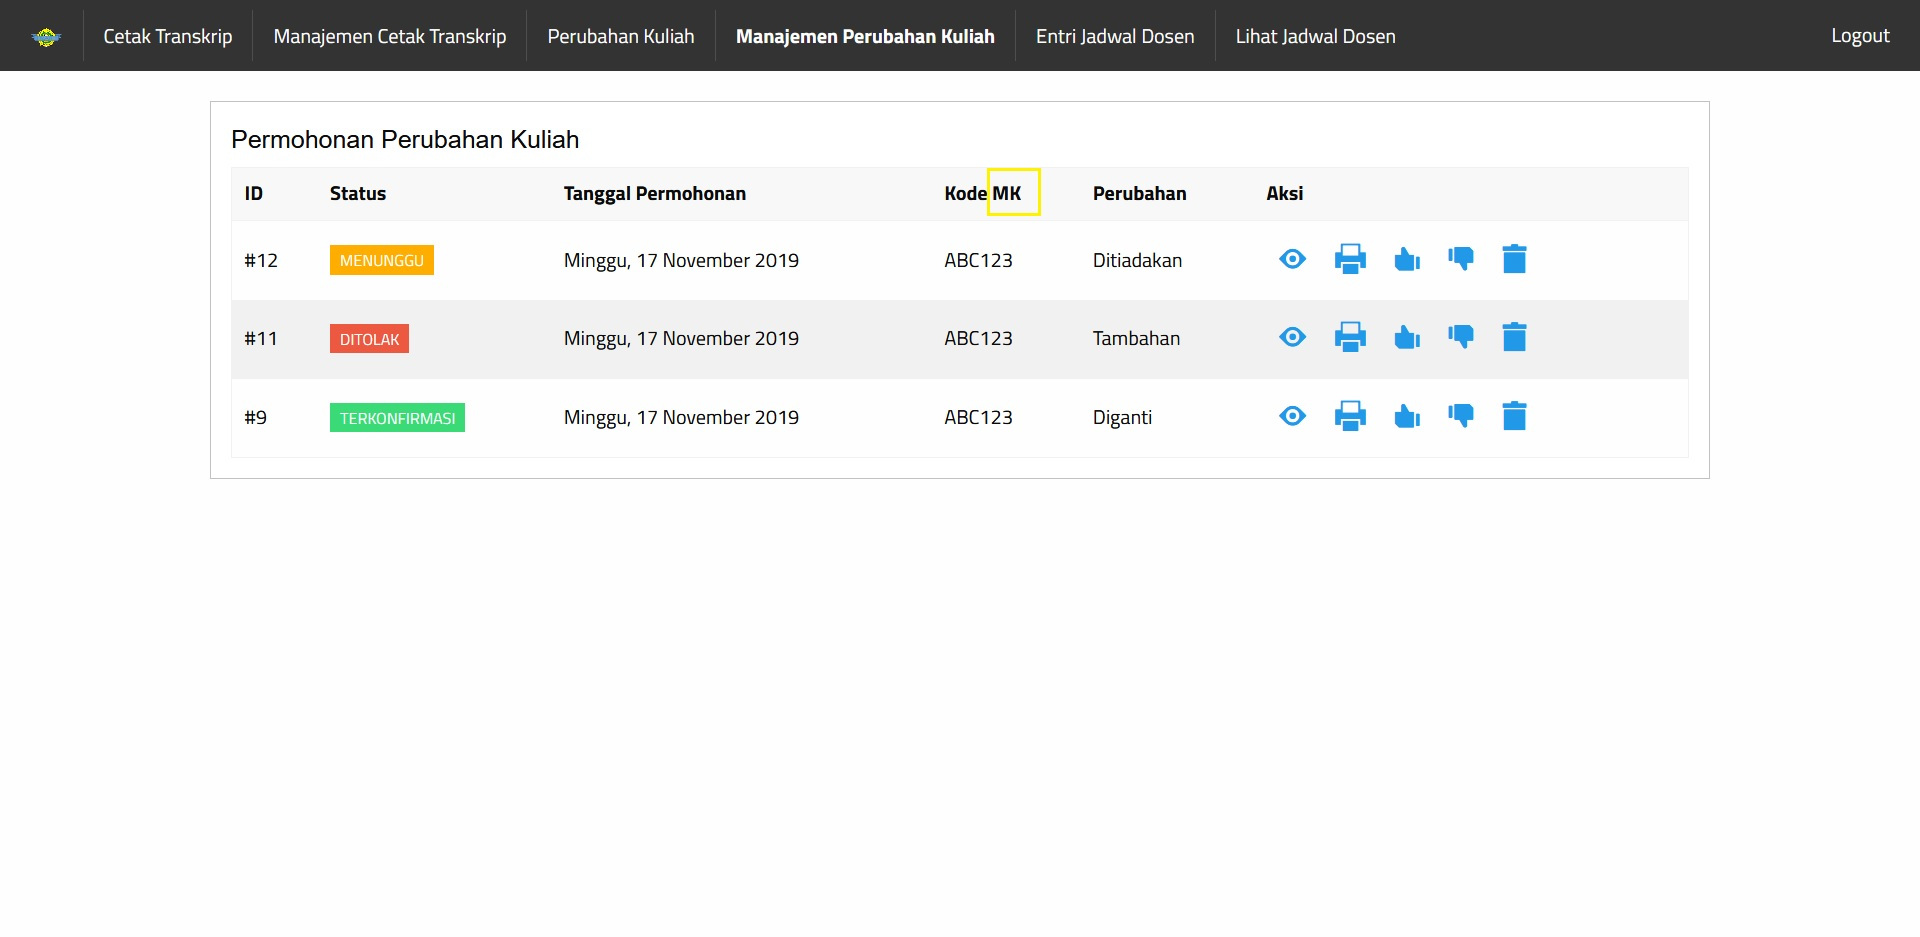
\includegraphics[scale=0.5]{kriteria-sukses-3-1-4-abbreviations-4}  
        \caption[Kriteria Sukses 3.1.4 - Singkatan pada Halaman Manajemen Perubahan Kuliah]{Kriteria Sukses 3.1.4 - Singkatan pada Halaman Manajemen Perubahan Kuliah}
        \label{fig:3.1.4_abbreviations_4}  
    \end{figure}
    Tautan untuk halaman yang bermasalah: 
    
    \url{https://bluetape.azurewebsites.net/PerubahanKuliahManage}.

    \item Pada halaman entri jadwal dosen terdapat singkatan "XLS". Letak kesalahan dapat dilihat pada potongan kode \ref{lst:3.1.4_singkatan_pada_halaman_entri_jadwal_dosen}. Contoh tampilan pada halaman web dapat dilihat pada gambar \ref{fig:3.1.4_abbreviations_5}.
    \begin{lstlisting}[frame=single, label={lst:3.1.4_singkatan_pada_halaman_entri_jadwal_dosen}, language=HTML, caption=Kriteria Sukses 3.1.4 - Singkatan pada Halaman Entri Jadwal Dosen]
        <a href="/EntriJadwalDosen/deleteAll/export/" 
        class="alert button" 
        onClick="return konfirmasi();">Delete All</a>
        <a href="/EntriJadwalDosen/export/" 
        class="button">Ekspor ke XLS</a>
        <script>
    \end{lstlisting}

    \begin{figure}[H]
        \centering  
        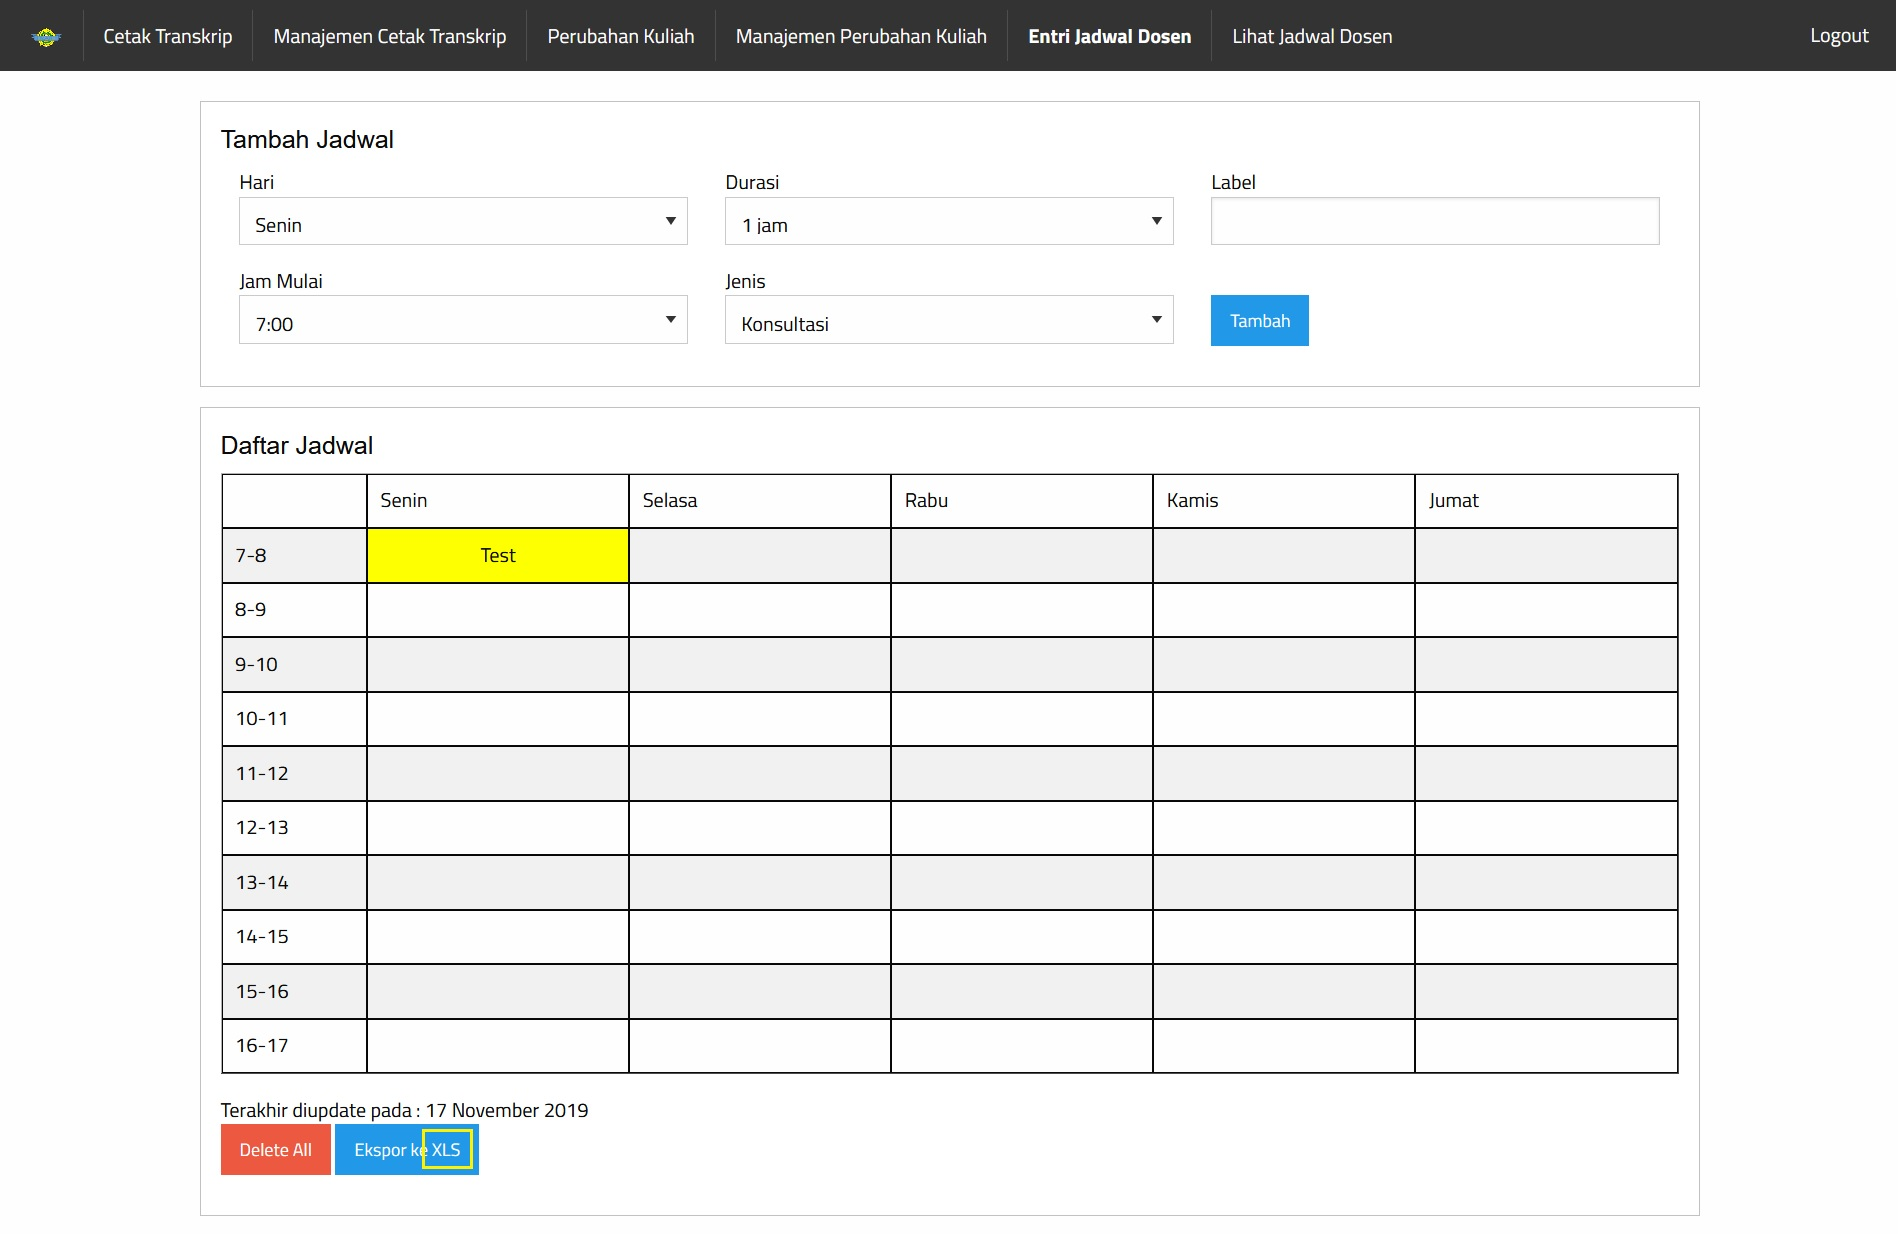
\includegraphics[scale=0.5]{kriteria-sukses-3-1-4-abbreviations-5}  
        \caption[Kriteria Sukses 3.1.4 - Singkatan pada Halaman Entri Jadwal Dosen]{Kriteria Sukses 3.1.4 - Singkatan pada Halaman Entri Jadwal Dosen}
        \label{fig:3.1.4_abbreviations_5}  
    \end{figure}
    Tautan untuk halaman yang bermasalah:
    
    \url{https://bluetape.azurewebsites.net/EntriJadwalDosen}.

    \item Pada halaman lihat jadwal dosen terdapat singkatan "XLS". Letak kesalahan dapat dilihat pada potongan kode \ref{lst:3.1.4_singkatan_pada_halaman_lihat_jadwal_dosen}. Contoh tampilan pada halaman web dapat dilihat pada gambar \ref{fig:3.1.4_abbreviations_6}.
    \begin{lstlisting}[frame=single, label={lst:3.1.4_singkatan_pada_halaman_lihat_jadwal_dosen}, language=HTML, caption=Kriteria Sukses 3.1.4 - Singkatan pada Halaman Lihat Jadwal Dosen]
        <?php
        }
        ?>
        <a href="/LihatJadwalDosen/export/" class="button">
            Ekspor ke XLS
        </a>
        </div> 
    \end{lstlisting}

    \begin{figure}[H]
        \centering  
        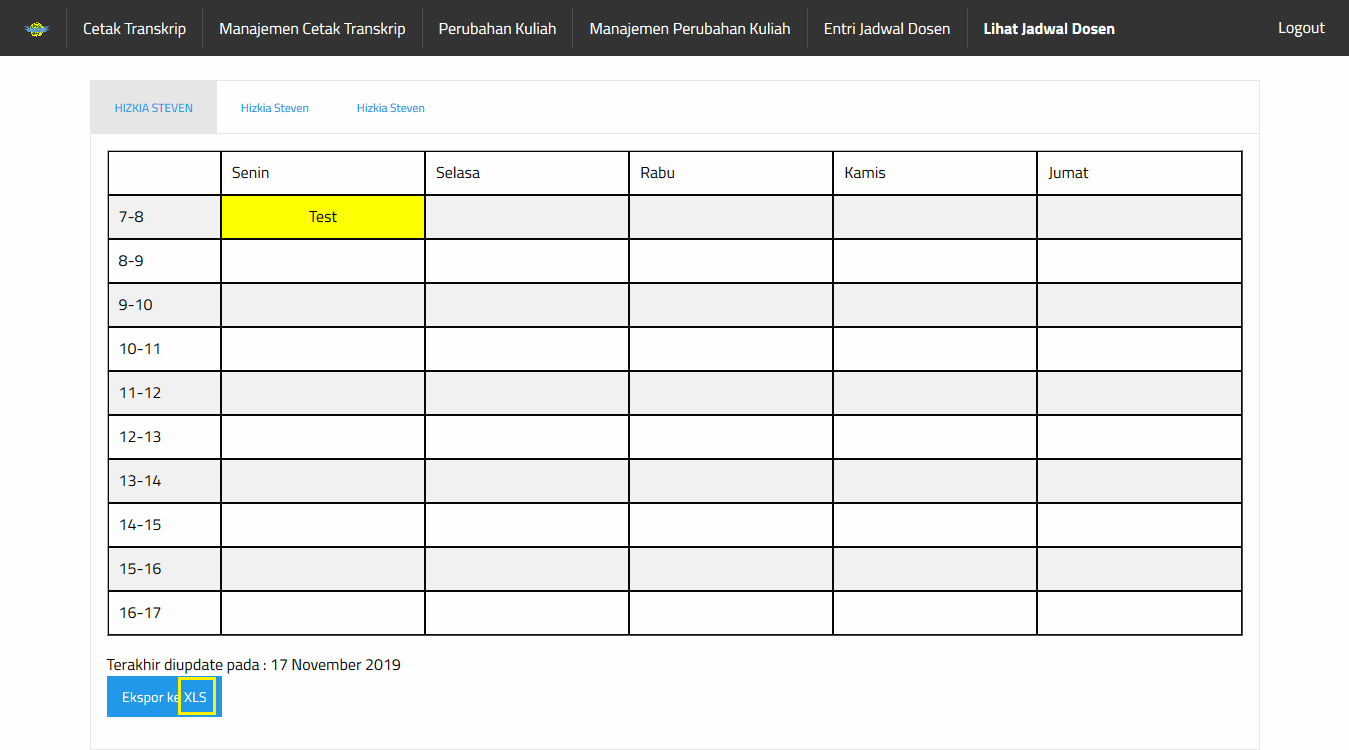
\includegraphics[scale=0.5]{kriteria-sukses-3-1-4-abbreviations-6}  
        \caption[Kriteria Sukses 3.1.4 - Singkatan pada Halaman Lihat Jadwal Dosen]{Kriteria Sukses 3.1.4 - Singkatan pada Halaman Lihat Jadwal Dosen}
        \label{fig:3.1.4_abbreviations_6}  
    \end{figure}
    Tautan untuk halaman yang bermasalah: 
    
    \url{https://bluetape.azurewebsites.net/LihatJadwalDosen}.
\end{itemize}

\paragraph{Kriteria Sukses 3.1.5 \textit{Reading Level}}
\label{par:kepatuhan_bluetape_kriteria_sukses_3.1.5}
(Sukses)\\

Kriteria ini sukses dipatuhi karena pada halaman web BlueTape tidak terdapat teks yang cukup kompleks dan membutuhkan kemampuan membaca yang lebih tinggi dari rata-rata.

\paragraph{Kriteria Sukses 3.1.6 \textit{Pronunciation}}
\label{par:kepatuhan_bluetape_kriteria_sukses_3.1.6}
(Sukses)\\

Kriteria ini sukses dipatuhi karena pada halaman web BlueTape setiap kata dapat dimengerti artinya tanpa pengguna perlu mengetahui cara mengucapkan kata tersebut.

\subsubsection{\textit{Predictable}}
\label{subsubsec:kepatuhan_bluetape_predictable}

\paragraph{Kriteria Sukses 3.2.1 \textit{On Focus}}
\label{par:kepatuhan_bluetape_kriteria_sukses_3.2.1}
(Sukses)\\

Kriteria ini sukses dipatuhi karena setiap komponen antarmuka pengguna yang menerima fokus, tidak menyebabkan perubahan konteks.

\paragraph{Kriteria Sukses 3.2.2 \textit{On Input}}
\label{par:kepatuhan_bluetape_kriteria_sukses_3.2.2}
(Sukses)\\

Kriteria ini sukses dipatuhi karena ketika pengguna mengubah setelan komponen antarmuka pengguna tidak terjadi perubahan konteks otomatis.

\paragraph{Kriteria Sukses 3.2.3 \textit{Consistent Navigation}}
\label{par:kepatuhan_bluetape_kriteria_sukses_3.2.3}
(Sukses)\\

Kriteria ini sukses dipatuhi karena bagian navigasi menu yang muncul berulang pada tiap halaman web BlueTape, muncul dalam urutan relatif yang sama setiap kali tampak.

\paragraph{Kriteria Sukses 3.2.4 \textit{Consistent Identification}}
\label{par:kepatuhan_bluetape_kriteria_sukses_3.2.4}
(Tidak Sukses)\\

Kriteria ini tidak sukses dipatuhi karena terdapat tombol yang memiliki fungsionalitas yang sama yaitu untuk menghapus namun diidentifikasikan dengan nama yang berbeda. Tombol yang dimaksud adalah tombol "Delete" pada bagian "Edit Jadwal" di halaman entri jadwal dosen. Tombol dengan fungsionalitas yang sama di halaman lain diidentifikasi dengan nama "Hapus". Contoh tampilan pada halaman web dapat dilihat pada gambar \ref{fig:3.2.4_consistent_identification}. 

\begin{figure}[H]
	\centering  
	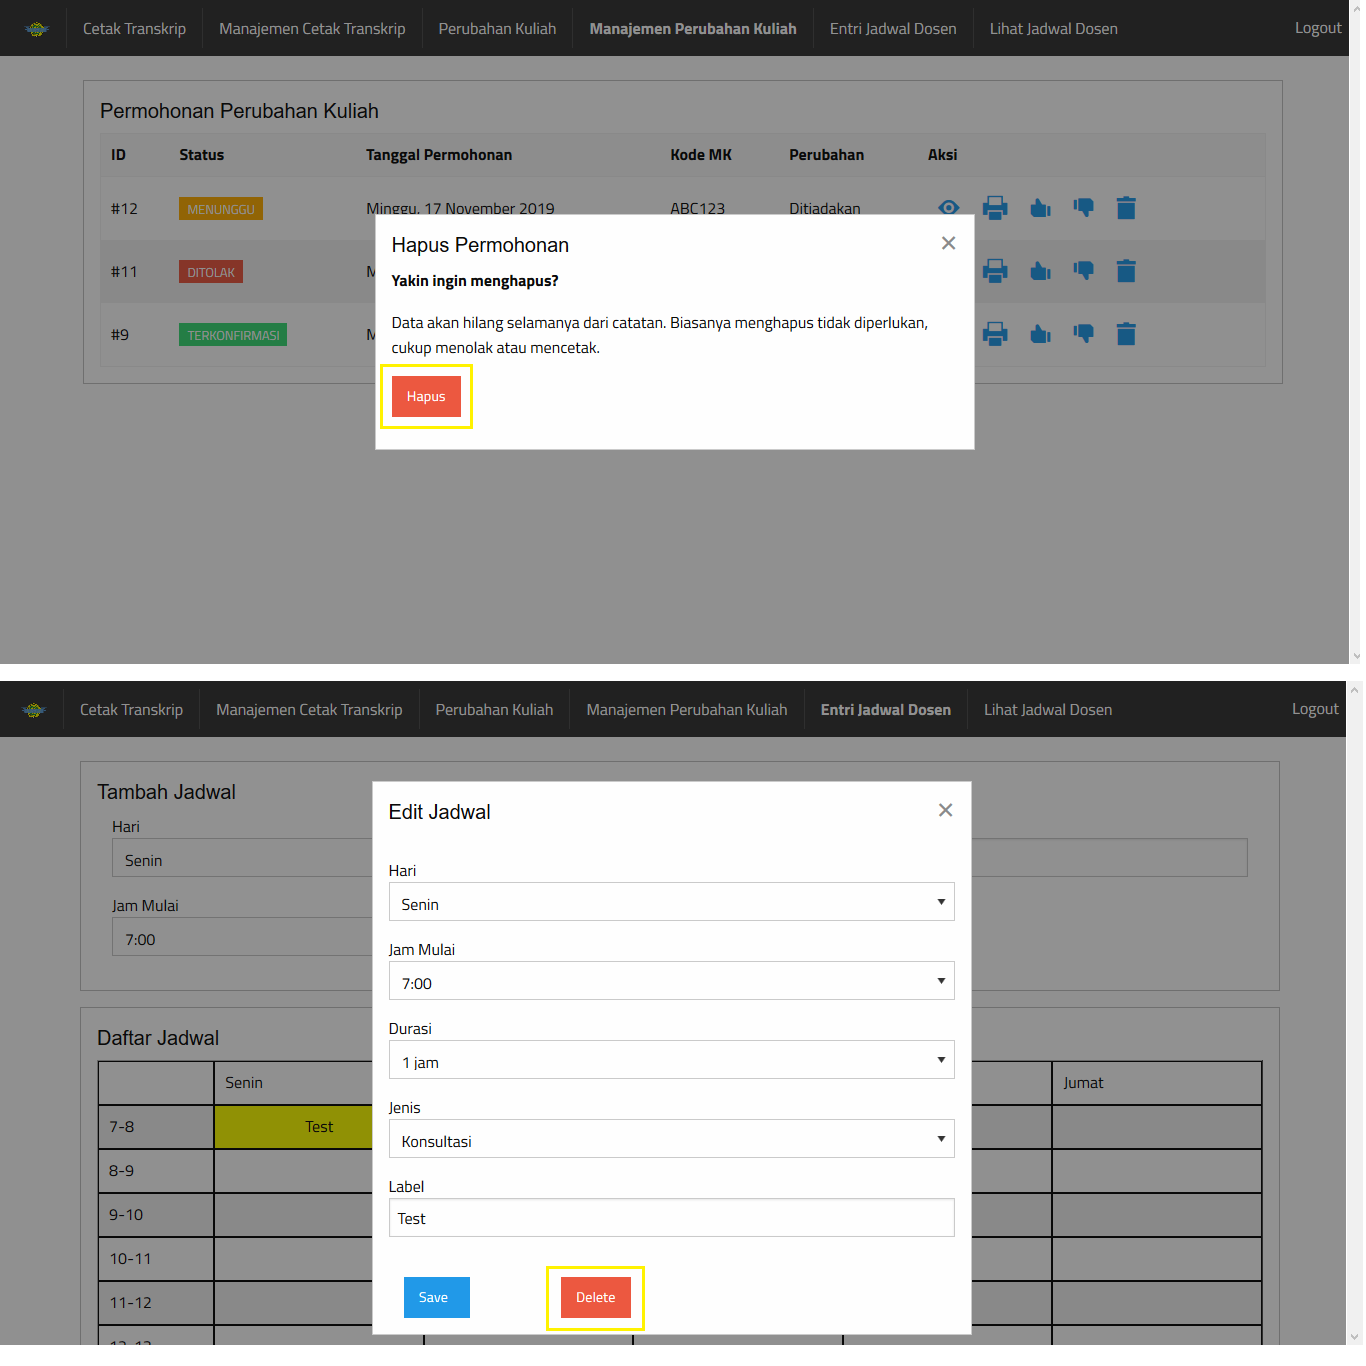
\includegraphics[scale=0.5]{kriteria-sukses-3-2-4-consistent-identification}  
	\caption[Kriteria Sukses 3.2.4 - Identifikasi pada Tombol]{Kriteria Sukses 3.2.4 - Identifikasi pada Tombol}
	\label{fig:3.2.4_consistent_identification}  
\end{figure}

Tautan untuk halaman yang bermasalah: 

\url{https://bluetape.azurewebsites.net/EntriJadwalDosen}.

\paragraph{Kriteria Sukses 3.2.5 \textit{Change on Request}}
\label{par:kepatuhan_bluetape_kriteria_sukses_3.2.5}
(Sukses)\\

Kriteria ini sukses dipatuhi karena setiap perubahan konteks hanya terjadi bila dilakukan oleh pengguna.

\subsubsection{\textit{Input Assistance}}
\label{subsubsec:kepatuhan_bluetape_input_assistance}

\paragraph{Kriteria Sukses 3.3.1 \textit{Error Identification}}
\label{par:kepatuhan_bluetape_kriteria_sukses_3.3.1}
(Sukses)\\

Kriteria ini sukses dipatuhi karena ketika terdapat eror masukan yang terdeteksi otomatis, \textit{item} yang eror diidentifikasi dan eror dijabarkan kepada pengguna dalam bentuk teks.

\paragraph{Kriteria Sukses 3.3.2 \textit{Labels or Instructions}}
\label{par:kepatuhan_bluetape_kriteria_sukses_3.3.2}
(Tidak Sukses)\\

Kriteria ini tidak sukses dipatuhi karena pada halaman entri jadwal dosen, setiap elemen masukan tidak memiliki label yang menjelaskan tujuan dari elemen tersebut. Contoh kesalahan dapat dilihat pada potongan kode \ref{lst:3.3.2_label_masukan_entri_jadwal_dosen}.

\begin{lstlisting}[frame=single, label={lst:3.3.2_label_masukan_entri_jadwal_dosen}, language=HTML, caption=Kriteria Sukses 3.3.2 - Tidak Terdapat Label pada Kolom Masukan di Halaman Entri Jadwal Dosen]
    <input type="hidden" name="csrf_token" 
    value="3c159eae7bc953dd591b679c080ed066"/>
    Hari
    <select name="hari">
\end{lstlisting}
Tautan untuk halaman yang bermasalah: 

\url{https://bluetape.azurewebsites.net/EntriJadwalDosen}.

\paragraph{Kriteria Sukses 3.3.3 \textit{Error Suggestion}}
\label{par:kepatuhan_bluetape_kriteria_sukses_3.3.3}
(Sukses)\\

Kriteria ini sukses dipatuhi karena ketika terdapat eror masukan yang terdeteksi otomatis, saran untuk mengoreksi eror tersebut disajikan kepada pengguna.

\paragraph{Kriteria Sukses 3.3.4 \textit{Error Prevention (Legal, Financial, Data)\\}}
\label{par:kepatuhan_bluetape_kriteria_sukses_3.3.4}
(Sukses)\\

Kriteria ini sukses dipatuhi karena pada halaman yang mengirim tanggapan pengguna, data yang dimasukkan oleh pengguna diperiksa terkait eror masukan dan pengguna dipersilakan untuk mengoreksinya.

\paragraph{Kriteria Sukses 3.3.5 \textit{Help}}
\label{par:kepatuhan_bluetape_kriteria_sukses_3.3.5}
(Tidak Sukses)\\

Kriteria ini tidak sukses dipatuhi karena pada halaman entri jadwal dosen, setiap elemen masukan tidak memiliki label yang menjelaskan tujuan dari elemen tersebut. Contoh kesalahan dapat dilihat pada potongan kode \ref{lst:3.3.5_label_masukan_entri_jadwal_dosen}.

\begin{lstlisting}[frame=single, label={lst:3.3.5_label_masukan_entri_jadwal_dosen}, language=HTML, caption=Kriteria Sukses 3.3.5 - Tidak Terdapat Label pada Kolom Masukan di Halaman Entri Jadwal Dosen]
    <input type="hidden" name="csrf_token" 
    value="3c159eae7bc953dd591b679c080ed066"/>
    Hari
    <select name="hari">
\end{lstlisting}
Tautan untuk halaman yang bermasalah: 

\url{https://bluetape.azurewebsites.net/EntriJadwalDosen}.

\paragraph{Kriteria Sukses 3.3.6 \textit{Error Prevention (All)}}
\label{par:kepatuhan_bluetape_kriteria_sukses_3.3.6}
(Sukses)\\

Kriteria ini sukses dipatuhi karena pada halaman yang mewajibkan pengguna mengirim informasi, data yang dimasukkan oleh pengguna diperiksa terkait eror masukan dan pengguna dipersilakan untuk mengoreksinya.

\subsection{\textit{Robust}}
\label{subsec:kepatuhan_bluetape_robust}

\subsubsection{\textit{Compatible}}
\label{subsubsec:kepatuhan_bluetape_compatible}

\paragraph{Kriteria Sukses 4.1.1 \textit{Parsing}}
\label{par:kepatuhan_bluetape_kriteria_sukses_4.1.1}
(Tidak Sukses)\\

Kriteria ini tidak sukses dipatuhi karena terdapat beberapa kesalahan, antara lain:

\begin{itemize}
    \item Pada halaman cetak transkrip, terdapat penggunaan \textit{tag "time"} yang kurang tepat yaitu tidak terdapat \textit{tag} akhir. Letak kesalahan dapat dilihat pada potongan kode \ref{lst:4.1.1_parsing_halaman_cetak_transkrip}.
    \begin{lstlisting}[frame=single, label={lst:4.1.1_parsing_halaman_cetak_transkrip}, language=HTML, caption=Kriteria Sukses 4.1.1 - Kesalahan Elemen pada Halaman Cetak Transkrip]
        <td>DPS</td>
        <td><time datetime="2019-11-17 17:55:16">
            Minggu, 17 November 2019</td>
        <td>Selesai</td>
    \end{lstlisting}
    Tautan untuk halaman yang bermasalah: 
    
    \url{https://bluetape.azurewebsites.net/TranskripRequest}.
    
    \item Pada halaman manajemen cetak transkrip, terdapat penggunaan atribut \textit{"readonly"} yang kurang tepat yaitu terdapat nilai \textit{"true"} untuk atribut tersebut. Letak kesalahan dapat dilihat pada potongan kode \ref{lst:4.1.1_parsing_halaman_manajemen_cetak_transkrip}.
    \begin{lstlisting}[frame=single, label={lst:4.1.1_parsing_halaman_manajemen_cetak_transkrip}, language=HTML, caption=Kriteria Sukses 4.1.1 - Kesalahan Elemen pada Halaman Manajemen Cetak Transkrip]
        <label>Email penjawab:
            <input type="text" value="7315020@student.unpar.ac.id"
            readonly="true"/>
        </label>
    \end{lstlisting}
    Tautan untuk halaman yang bermasalah: 
    
    \url{https://bluetape.azurewebsites.net/TranskripManage}.

    \item Pada halaman manajemen perubahan kuliah, terdapat penggunaan atribut \textit{"readonly"} yang kurang tepat yaitu terdapat nilai \textit{"true"} untuk atribut tersebut. Letak kesalahan dapat dilihat pada potongan kode \ref{lst:4.1.1_parsing_halaman_manajemen_perubahan_kuliah}.
    \begin{lstlisting}[frame=single, label={lst:4.1.1_parsing_halaman_manajemen_perubahan_kuliah}, language=HTML, caption=Kriteria Sukses 4.1.1 - Kesalahan Elemen pada Halaman Manajemen Perubahan Kuliah]
        <label>Email penjawab:
            <input type="text" value="7315020@student.unpar.ac.id" 
            readonly="true"/>
        </label>
    \end{lstlisting}
    Tautan untuk halaman yang bermasalah: 
    
    \url{https://bluetape.azurewebsites.net/PerubahanKuliahManage}.

    \item Pada halaman entri jadwal dosen, terdapat elemen \textit{"HTML"} yang penempatannya tidak tepat yaitu \textit{tag "div"} berada sebelum \textit{tag "body"}. Letak kesalahan dapat dilihat pada potongan kode \ref{lst:4.1.1_parsing_halaman_entri_jadwal_dosen}.
    \begin{lstlisting}[frame=single, label={lst:4.1.1_parsing_halaman_entri_jadwal_dosen}, language=HTML, caption=Kriteria Sukses 4.1.1 - Kesalahan Elemen pada Halaman Entri Jadwal Dosen]
        </head>
        <div class="row">
        </div>        
        <body>
    \end{lstlisting}
    Tautan untuk halaman yang bermasalah: 
    
    \url{https://bluetape.azurewebsites.net/EntriJadwalDosen}.

    \item Pada halaman lihat jadwal dosen, terdapat \textit{tag "a"} yang memiliki atribut yang tidak tepat yaitu atribut \textit{"a"}. Letak kesalahan dapat dilihat pada potongan kode \ref{lst:4.1.1_parsing_halaman_lihat_jadwal_dosen}. Selain itu, terdapat \textit{tag "div"} buka yang tidak disertai dengan \textit{tag "div"} tutup karena jumlah keduanya tidak sama.
    \begin{lstlisting}[frame=single, label={lst:4.1.1_parsing_halaman_lihat_jadwal_dosen}, language=HTML, caption=Kriteria Sukses 4.1.1 - Kesalahan Elemen pada Halaman Lihat Jadwal Dosen]
        <li class="tabs-title">
            <a a href="#hal1">Hizkia Steven</a>
        </li>
        <li class="tabs-title">
            <a a href="#hal2">Hizkia Steven</a>
        </li>
    \end{lstlisting}
    Tautan untuk halaman yang bermasalah: 
    
    \url{https://bluetape.azurewebsites.net/LihatJadwalDosen}.

\end{itemize}

\paragraph{Kriteria Sukses 4.1.2 \textit{Name, Role, Value}}
\label{par:kepatuhan_bluetape_kriteria_sukses_4.1.2}
(Tidak Sukses)\\

Kriteria ini tidak sukses dipatuhi karena pada halaman lihat jadwal dosen terdapat \textit{tag "a"} yang belum memiliki atribut \textit{role} yang tepat, yaitu pada bagian nama dosen yang sedang dipilih untuk ditampilkan jadwalnya. Letak kesalahan dapat dilihat pada potongan kode \ref{lst:4.1.2_role_halaman_lihat_jadwal_dosen}.

\begin{lstlisting}[frame=single, label={lst:4.1.2_role_halaman_lihat_jadwal_dosen}, language=HTML, caption=Kriteria Sukses 4.1.1 - Atribut \textit{Role} pada Halaman Lihat Jadwal Dosen]
    <li class="tabs-title is-active">
        <a href="#hal0" aria-selected="true">HIZKIA STEVEN</a>
    </li> 
\end{lstlisting}
Tautan untuk halaman yang bermasalah: 

\url{https://bluetape.azurewebsites.net/LihatJadwalDosen}.

\paragraph{Kriteria Sukses 4.1.3 \textit{Status Messages}}
\label{par:kepatuhan_bluetape_kriteria_sukses_4.1.3}
(Tidak Sukses)\\

Kriteria ini tidak sukses dipatuhi karena setiap pesan status yang ditampilkan kepada pengguna tidak memiliki atribute \textit{"role"} dengan nilai \textit{"alert"} sehingga teknologi alat bantu tidak dapat mengidentifikasi serta menginformasikan pesan tersebut kepada pengguna. Letak kesalahan dapat dilihat pada potongan kode \ref{lst:4.1.3_pesan_status}.

\begin{lstlisting}[frame=single, label={lst:4.1.3_pesan_status}, language=PHP, caption=Kriteria Sukses 4.1.3 - Atribut pada Pesan Status]
    <?php if (isset($_SESSION['error'])): ?>
        <div class="callout alert"><?= $_SESSION['error'] ?></div>
    <?php endif; ?>
    <?php if (isset($_SESSION['info'])): ?>
        <div class="callout primary"><?= $_SESSION['info'] ?></div>
    <?php endif; ?>
\end{lstlisting}